\documentclass[bibtotoc,liststotoc,BCOR=5mm,DIV=12]{scrbook}
% \documentclass[a4paper,twoside,openright,11pt]{book}

% use this declaration to set specific page margins
%\usepackage[a4paper , lmargin = {2.7cm} , rmargin = {2.9cm} , tmargin = {2.7cm} , bmargin = {4.6cm} ]{geometry}
\usepackage[a4paper]{geometry}
\usepackage{pdfpages}
\usepackage{sethesis}

\usepackage[english, ngerman]{babel}
% always use 'Figure' instead of german 'Abbildung' in captions
\addto\captionsngerman{\renewcommand{\figurename}{Figure}}
\addto\captionsenglish{\renewcommand{\figurename}{Figure}}
\usepackage[round,authoryear]{natbib}  % author-year citations
% \usepackage{bibgerm}        		% german references (commented out - conflicts with natbib)
\usepackage[T1]{fontenc} % german characters
\usepackage{amsmath} % math environments and symbols
\usepackage{siunitx} % units and quantities
\usepackage{graphicx} 				% it's recommended to use PDF images but you can use JPG or PNG as well
\usepackage{url}            		% format URLs
\usepackage{hyperref} 				% create hyperlinks
\usepackage{listings, color}	% for source code
\usepackage{subfig}						% two figures next to each other (example: figure 3a), figure 3b)
\usepackage{scrlayer-scrpage}					% header and footer line
\usepackage{todonotes}
\usepackage{amssymb} % for \checkmark

% Paragraph spacing: add space between paragraphs within sections
\setlength{\parskip}{0.5em}

% Figure caption formatting: bold Figure label, no indent on wrapped lines
\usepackage{caption}
\captionsetup[figure]{labelfont=bf, format=plain, justification=justified, singlelinecheck=false}
\captionsetup[table]{labelfont=bf, format=plain, justification=justified, singlelinecheck=false}

% header and footer line - no header & footer line on pages where a new chapter starts
% \pagestyle{scrheadings}
% \ohead{Design and Implementation of X}
% \ihead{Your Name}
% \ofoot[]{\thepage}
% \ifoot{Thesis, TU Berlin, Fachgebiet D2IP, 2024}

% configure link appearance: red outlines for structural links, green for citations
\hypersetup{
  colorlinks=false,
  pdfborder={0 0 1},
  linkbordercolor={1 0 0},   % sections, figures, etc. (red)
  citebordercolor={0 1 0},   % citations (green)
  urlbordercolor={0 0 1}     % URLs (blue)
}

% set paths where images are stored
\graphicspath{{./img/}{./img/data-insight/}{./img/imaestro-data/}{./img/training-data-insight/}{./img/training-results/}{./img/training-results/treesatai/}{./img/training-results/imaestro-baseline/}{./img/training-results/imaestro-mtl/}}

\uniname{Technische Universität Berlin}
\fachgebiet{Computer Vision and Remote Sensing}
% \institut{Institut für Praktische Informatik}
\fachbereich{Fakultät IV Elektrotechnik und Informatik}
\studiengang{MSc. Computer Engineering}
% Angaben zur Arbeit
\author{Siyu Xiao}
\title{Multitask Learning for Extraction of Bio-/Geo Physical Parameters from SAR Imagery}
% \englishtitle{<Englischer Titel der Arbeit>}
\ort{Berlin}
\thesistype{Master's Thesis}
%\thesistype{Masterarbeit}
% Pruefer
\erstpru{Prof. Dr.-Ing. Olaf Hellwich}
\zweitpru{Dr.-Ing. Ronny Hänsch}
\betreu{Ragini Bal Mahesh}
\datum{<Submission date>}

\begin{document}
% ---------------------------------------------------------------
\renewcommand{\chaptername}{Chapter}

\frontmatter

\maketitle
% \frontmatter
    
    
    \newpage

\thispagestyle{empty}

\chapter*{Declaration of Authorship}
\vspace*{1cm}

\noindent
I hereby declare that I have written this thesis independently and without unauthorized external assistance. All sources and aids used are indicated in the thesis, and all passages taken verbatim or in spirit from other works are clearly marked as such.

\vspace{2cm}
\noindent
Name, student ID\\
\vspace{0.5cm}

\noindent
Berlin, ..................................\\
\vspace{1cm}\\
Signature ..................................
\vspace{3cm}
 
    \thispagestyle{empty}
    \cleardoublepage
    
    
    \chapter*{Abstract}

\vspace{1cm}

This thesis investigates multitask learning for forest monitoring from Sentinel-1 SAR imagery. The main question is whether a single model can estimate multiple forest attributes more efficiently than separate single-task models, and how physics-aware constraints can improve learning.Two datasets were used for experiments. First, the TreeSatAI benchmark was extended with canopy height labels from German LiDAR data, creating TreeSatAI-CHM for joint species classification and height regression. Second, the iMAESTRO dataset provided genus segmentation, height, and biomass labels, enabling tests of allometric constraints that couple height and biomass predictions. The experiments show that multitask learning achieves comparable or slightly better performance than single-task baselines while using fewer parameters and less inference time. Gradient analysis reveals that tasks generally align in deeper network layers while occasionally conflicting in early layers. Physics-aware constraints successfully guide related tasks (height and biomass) toward consistent predictions that respect ecological relationships. The main challenges are balancing tasks with different loss scales and managing task asymmetry. Uncertainty weighting and gradient analysis both address these issues effectively. While absolute performance improvements are modest due to C-band SAR's inherent limits, multitask learning offers a practical solution for operational forest monitoring where computational efficiency matters.

    \thispagestyle{empty}
    \cleardoublepage
    
    \renewcommand{\contentsname}{Contents}
    
    \tableofcontents
    \thispagestyle{empty}
    
    % \listoffigures
    % \thispagestyle{empty}
    
    % \listoftables
    % \thispagestyle{empty}
    
% --------------------------------------------------------------

\mainmatter % comment single chapters for faster compilation
    \chapter{Introduction}
\label{chap:introduction}

Forests play a central role in ecosystem preservation, and reliable methods for monitoring forest structure at large scales are essential for resource management. Traditional forest inventory relies on field surveys where trained personnel measure attributes like tree height, diameter, and species composition. These methods are accurate at the plot level but costly and impractical for regional or continental assessments.

Remote sensing offers a scalable alternative. Optical sensors such as Landsat and Sentinel-2 have been widely used for vegetation monitoring through spectral reflectance analysis. However, optical imagery is limited by cloud cover, with approximately 67\% of Earth's surface obscured at any given time, and tropical forests experiencing persistent cloud conditions for much of the year. Synthetic Aperture Radar (SAR) addresses this limitation through active microwave sensing that operates regardless of weather or illumination conditions. The European Space Agency's Sentinel-1 mission provides freely available C-band SAR data with global coverage and six-day revisit times. Research has demonstrated that SAR backscatter contains information about forest vertical structure, with studies achieving correlation coefficients of 0.72--0.84 for canopy height prediction when combining Sentinel-1 with auxiliary data sources \cite{li2020canopy,wang2022canopy}.

Deep learning has advanced remote sensing image analysis, with convolutional neural networks and encoder--decoder architectures achieving strong performance for classification and regression tasks. Lang et al.~\cite{lang2023canopy} produced a global canopy height map at 10~m resolution by fusing GEDI LiDAR with Sentinel-2 imagery using deep learning, demonstrating the potential of neural networks for large-scale forest parameter estimation. Most existing approaches, however, train separate models for individual forest parameters, overlooking relationships among attributes like species identity and canopy height. Multitask learning offers an alternative paradigm where a single model predicts multiple parameters simultaneously, potentially exploiting shared representations to improve accuracy across related tasks \cite{vandenhende2022mtlsurvey}.

A key challenge for developing multitask models is data availability. Existing benchmark datasets for forest remote sensing typically focus on single tasks: some provide species labels without height annotations, others offer LiDAR-derived heights without species information. This fragmentation limits research on multitask approaches that could exploit the interdependencies among forest attributes. The TreeSatAI benchmark \cite{ahlswede2023treesatai} provides Sentinel-1 imagery with species labels for German forests, covering 20 European tree species grouped into 15 genera across Lower Saxony. However, it does not include height information. Extending this established benchmark with canopy height labels derived from official German LiDAR elevation products represents a pathway to enable multitask learning research while maintaining data quality and spatial coverage.

This thesis investigates multitask learning for forest attribute estimation from Sentinel-1 SAR imagery. This thesis uses two datasets to address different aspects of multitask learning. The primary focus is on TreeSatAI-CHM, which extends the established TreeSatAI benchmark with canopy height labels derived from German LiDAR data. This dataset enables investigation of fundamental multitask learning challenges like loss scale mismatches, gradient conflicts, and parameter sharing strategies in a controlled environment with well-recognized benchmark data. Additionally, the iMAESTRO dataset provides comprehensive reference data for genus segmentation, canopy height, and biomass estimation, enabling testing of physics-aware deep learning through allometric constraints that link height and biomass.

This thesis addresses the following questions:

\begin{enumerate}
    \item Can TreeSatAI be extended with canopy height labels?
    \item How do shared encoders learn features for multiple tasks?
    \item When do gradient conflicts happen and how to manage them?
    \item Does multitask learning match or beat single-task baselines?
    \item Can physics-aware constraints improve multitask learning?
\end{enumerate}

The main contributions of this thesis are:

\begin{itemize}
    \item Extended the TreeSatAI benchmark with canopy height labels derived from official German LiDAR elevation products, creating TreeSatAI-CHM for multitask learning research.
    \item Developed multitask architectures for joint species classification and height regression from Sentinel-1 SAR imagery.
    \item Demonstrated physics-aware multitask learning by incorporating allometric constraints linking canopy height and biomass.
    \item Provided quantitative evidence of task interactions showing where tasks align (deeper layers) and conflict (early layers) in shared architectures.
\end{itemize}

The remainder of this thesis is organized as follows. Chapter~\ref{chap:background} provides the theoretical background, covering SAR remote sensing for forest monitoring, multitask learning principles and applications, and dataset availability for forest parameter extraction. Chapter~\ref{chap:methodik} describes the methodology, including dataset preparations and experimental design. The TreeSatAI-CHM dataset construction involves generating canopy height models from digital terrain and surface models, aligning them to the TreeSatAI patch grid. Model architectures include MLP and U-Net baselines, and a MultiTaskUNet with shared encoder and task-specific decoders for joint learning. The iMAESTRO dataset provides forest data with genus segmentation, canopy height, and biomass labels, enabling testing of allometric constraints. Chapter~\ref{chap:experiments} presents experiments and results, focusing on TreeSatAI-CHM for understanding fundamental multitask learning dynamics, with iMAESTRO experiments demonstrating physics-aware deep learning. Chapter~\ref{chap:discussion} concludes with key findings, connecting back to the thesis questions.

    \chapter{Theoretical Background}
\label{chap:background}

This chapter provides the theoretical foundations for this thesis, covering three main areas. Section~\ref{sec:sar_forest} examines SAR remote sensing for forest parameter estimation, including the physical basis of radar-vegetation interactions and existing approaches for height and species extraction. Section~\ref{sec:mtl_rs} reviews multitask learning principles and their application in remote sensing contexts. Section~\ref{sec:datasets} discusses dataset availability for forest monitoring research and the challenges of obtaining multitask annotations.

\section{SAR Imagery for Forest Parameter Estimation}
\label{sec:sar_forest}

Synthetic Aperture Radar has become a valuable tool for forest monitoring because it offers capabilities that optical sensors cannot match. The main advantage is that SAR actively transmits microwave pulses and records the backscattered signal, which means it can acquire imagery regardless of sunlight or weather conditions. This all-weather, day-and-night capability is especially useful for monitoring forests in regions with frequent cloud cover, where optical data is often unavailable \cite{moreira_tutorial_2013}.

How SAR interacts with forest canopies reveals information about vegetation structure that optical sensors miss. The key factor is wavelength, which determines how deeply the signal penetrates: X-band signals interact mainly with leaves and small branches at the canopy surface, C-band (used by Sentinel-1) penetrates into the upper canopy structure, while L-band and P-band wavelengths can reach tree trunks and even the ground surface. This penetration capability allows SAR to sense vertical forest structure, making it sensitive to parameters like canopy height.

Research has demonstrated the potential of SAR data for forest canopy height estimation. ~\cite{li_high-resolution_2020} showed that coupling ICESat-2 LiDAR with Sentinel-1, Sentinel-2 and Landsat-8 data achieved correlation coefficients of 0.78 for canopy height prediction, with the addition of Sentinel-1 backscattering coefficients contributing positively to model performance. Similarly, ~\cite{wei_forest_2024} found that synergizing ICESat-2, Sentinel-1, Sentinel-2 and topographic information using Random Forest achieved RMSE values of 3.15--3.37~m for different forest types in China. \cite{srivastava_joint_2017} demonstrated joint estimation of multiple forest parameters from SAR data, showing that coupled predictions can improve accuracy through shared feature learning. The VH and VV polarization channels from Sentinel-1 were validated as important predictors, with cross-polarized backscatter (VH) showing stronger sensitivity to vegetation structure due to its response to volume scattering.

Deep learning approaches have recently advanced canopy height estimation capabilities. \cite{lang_high-resolution_2023} developed a probabilistic deep learning model that fused sparse GEDI LiDAR data with Sentinel-2 optical images, producing global canopy height maps at 10~m resolution with RMSE of 7.9~m. \cite{castro_deep_2024} found that combining seasonal Sentinel-1 and optical features with PALSAR data yielded $R^2$ of 0.72 and RMSE of 3.43~m for northern forests, noting that SAR data provides valuable structural insights complementary to optical spectral information. For SAR-specific approaches, \cite{mahesh_forest_2024} investigated forest height estimation using TanDEM-X InSAR features with deep learning, demonstrating that interferometric coherence and backscatter can be combined in convolutional neural networks for height prediction, achieving RMSE of 6.12~m with volumetric decorrelation as the primary input feature. \cite{mahesh_deep_2023} further explored deep learning for forest canopy height estimation from SAR, showing that convolutional architectures can extract height-relevant features from InSAR products and single-look complex SAR images. Recent work has also explored fusing physical models with deep learning. \cite{wei_forest_2024} proposed using InSAR coherence as an indicator for forest canopy height estimation, establishing relationships between coherence stability and vegetation structure. \cite{mahesh_better_2025} developed CoHNet, an end-to-end framework that fuses physical models with deep learning by optimizing volume decorrelation through a physics-aware training loss, demonstrating that incorporating physical constraints improves forest height estimation accuracy compared to purely data-driven methods.

For tree species classification from SAR, research has shown that texture features, temporal patterns, and polarimetric decomposition products provide discriminative information. The TreeSatAI benchmark \cite{ahlswede_treesatai_2023} demonstrated that Sentinel-1 data contributes to species classification when combined with optical imagery, though optical sensors typically achieve higher accuracy when used alone. \cite{dostalova_european_2021} achieved European-wide forest classification using Sentinel-1 data, demonstrating the potential of C-band SAR for vegetation type discrimination. \cite{udali_assessing_2021} assessed forest type and tree species classification using Sentinel-1 C-band SAR data in southern Sweden, finding that backscatter coefficients from VV and VH polarizations combined with temporal features achieved classification accuracies up to 85\% for dominant species. More recently, \cite{grace_tree_2024} explored tree species classification using machine learning and 3D tomographic SAR data in northern Europe, demonstrating that tomographic features extracted from multi-baseline SAR acquisitions provide additional discriminative power for species identification.

The C-band wavelength of Sentinel-1 presents both opportunities and challenges for forest applications. The free availability, global coverage, and frequent revisit make Sentinel-1 data accessible for operational applications in a way that commercial SAR sensors are not. However, C-band has limited penetration into dense forest canopies compared to longer wavelength systems like L-band ALOS-2 PALSAR, which affects sensitivity to height in mature forests with closed canopies. Despite these limitations, C-band SAR has shown useful correlations with canopy height, particularly when temporal features or texture information are exploited.

The reason for investigating SAR-only approaches relates to operational constraints. While optical-SAR fusion generally improves model performance, the requirement for cloud-free optical imagery limits how frequently predictions can be made. Approximately 67\% of Earth's surface is covered by clouds at any given time, and in tropical forests where cloud cover persists throughout much of the year, waiting for clear optical scenes may delay monitoring by weeks or months. \cite{wu_segcr_2025} demonstrated that semantic change detection can be performed effectively using SAR data alone, highlighting the value of all-weather monitoring capabilities for time-sensitive applications. A robust SAR-based approach would enable continuous monitoring regardless of atmospheric conditions, supporting applications in forest change detection, degradation monitoring, and inventory updating where timeliness is important. Furthermore, developing SAR-only methods has value for understanding what information SAR actually provides about forests. When SAR is always combined with optical data, it becomes difficult to isolate the contribution of radar features to the prediction. By investigating SAR-only models, this research aims to clarify the extent to which structural information in radar backscatter can support forest parameter extraction.

\section{Multitask Learning in Remote Sensing}
\label{sec:mtl_rs}

Multitask learning is a machine learning approach where a single model learns to perform multiple related tasks at the same time, using shared representations to boost performance across all tasks. The core idea is straightforward: when tasks are related, they can benefit from learning common features together rather than separately. This joint learning acts as a form of regularization, helping the model avoid overfitting to task-specific noise and improving its ability to generalize.

\subsection{Deep Learning Architectures for Multitask Learning}

\cite{vandenhende_multi-task_2021} provided a comprehensive survey of MTL approaches for dense prediction tasks in computer vision, establishing a taxonomy of architectural strategies. Figure~\ref{fig:mtl-basics} illustrates this taxonomy, showing how different MTL architectures organize the flow of information between tasks. The survey identifies two fundamental paradigms for parameter sharing in deep multitask networks: hard parameter sharing and soft parameter sharing.

\begin{figure}[htbp]
\centering
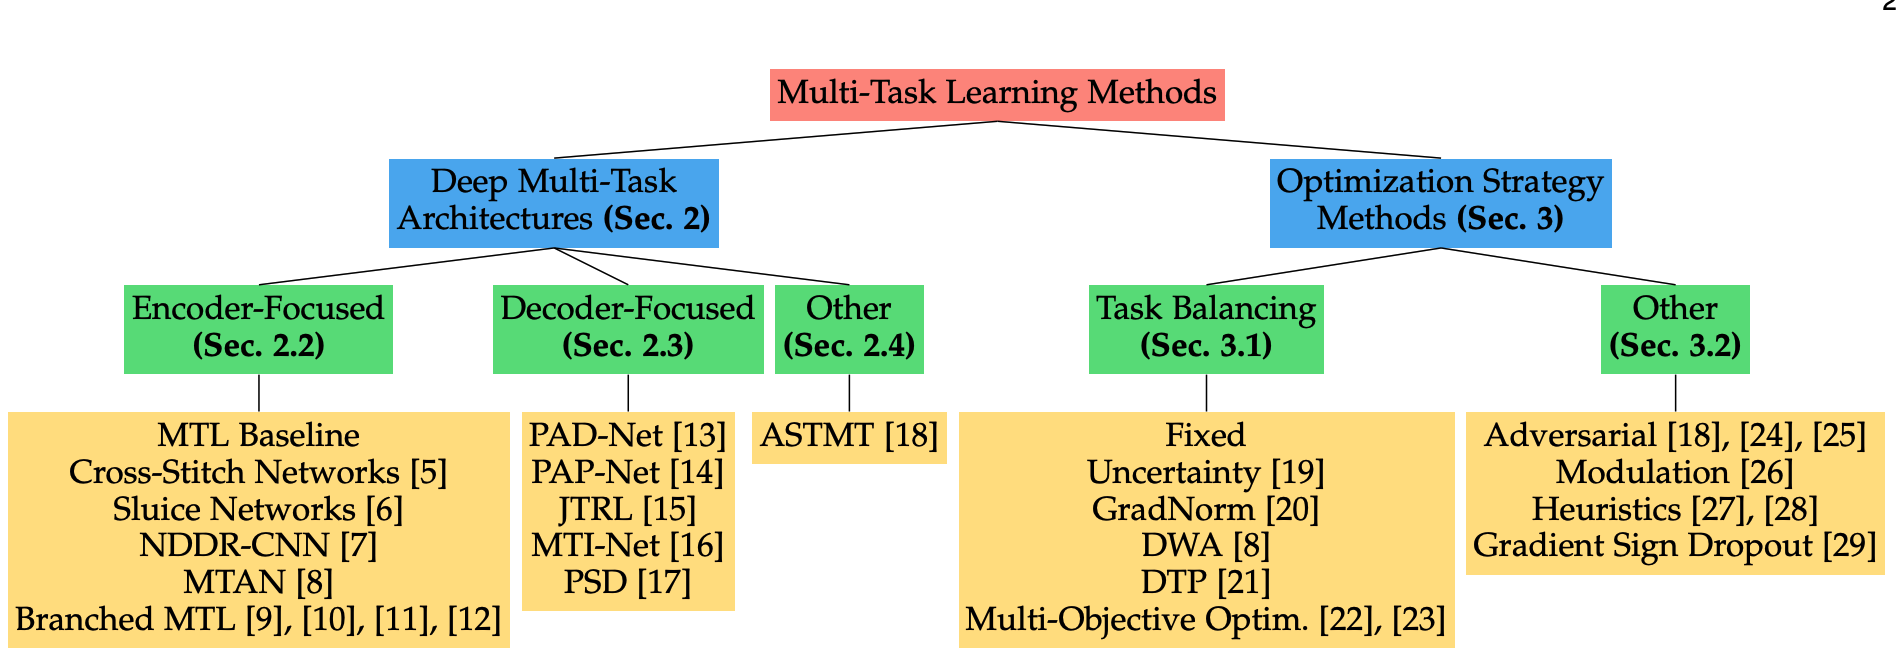
\includegraphics[width=0.9\textwidth]{img/mtl-basics.png}
\caption{A taxonomy of deep learning approaches for jointly solving multiple dense prediction tasks. The figure shows different architectural strategies including hard parameter sharing (shared encoder with task-specific decoders), soft parameter sharing (task-specific networks with cross-connections), and attention-based approaches. Adapted from \cite{vandenhende_multi-task_2021}.}
\label{fig:mtl-basics}
\end{figure}

\textbf{Hard parameter sharing} is the most common approach. Here, all tasks share the same encoder network that extracts features from the input, while each task gets its own decoder (or output head) to produce task-specific predictions. This setup forces the shared encoder to learn representations that are useful for all tasks simultaneously. The main advantage is efficiency: you only need one encoder instead of multiple separate networks. The challenge is that the shared encoder must balance the needs of different tasks, which can be difficult when tasks have conflicting requirements.

\textbf{Soft parameter sharing} takes a different approach. Each task has its own network with its own parameters, but these networks communicate with each other through specialized connection mechanisms. This allows tasks to share information selectively rather than forcing everything through a single shared encoder. \cite{misra_cross-stitch_2016} introduced cross-stitch networks, which use learnable linear combinations to mix activations between task-specific networks at multiple layers. The cross-stitch units learn how much information each task should receive from the other tasks' representations, enabling flexible sharing patterns that can adapt during training. The Multi-Task Attention Network (MTAN) uses attention mechanisms to learn task-specific feature-level attention. Each task has its own attention network that selectively focuses on relevant features from a shared backbone, allowing the model to automatically determine which features are important for each task.

The choice between hard and soft parameter sharing involves trade-offs. Hard sharing is more parameter-efficient and provides stronger regularization, but it can suffer when tasks are only weakly related or have conflicting optimization requirements. Soft sharing offers more flexibility and can better handle diverse tasks, but requires more parameters and careful design of the cross-task communication mechanisms. The optimal choice depends on task relatedness, available training data, and computational constraints.

\subsection{Multitask Learning for Forest Monitoring}

In remote sensing, multitask learning has been applied to various forest monitoring problems, though most work focuses on optical imagery. \cite{plotnikov_multitask_2025} explored multitask learning for estimating primary forest characteristics using Sentinel-2 data, demonstrating that jointly predicting multiple forest attributes (such as tree height, diameter, and basal area) from optical imagery improves estimation accuracy compared to single-task models. Their approach used a shared convolutional encoder with task-specific regression heads, showing that structural forest parameters share underlying spectral patterns that can be exploited through joint learning.

\cite{cui_mtscd-net_2023} proposed MTSCD-Net, a network based on multitask learning for semantic change detection of bitemporal remote sensing images. The architecture combines binary change detection (identifying where changes occurred) with semantic change detection (classifying the type of change) as complementary tasks. \cite{tao_multi-task_2025} developed a multitask learning framework with enhanced cross-level semantic consistency for multi-level land cover classification. Their approach addresses the hierarchical nature of land cover classification systems. By jointly learning classifications at multiple hierarchical levels and enforcing semantic consistency between levels, the model achieves improved accuracy at both coarse and fine scales compared to training separate classifiers for each level. Recent advances in multitask learning architectures have explored state-space models, with \cite{shen_learning_2025} demonstrating that Mamba-based architectures can effectively handle multiple dense prediction tasks in remote sensing through efficient long-range dependency modeling. \cite{liu_associatively_2022} proposed associative learning mechanisms that enable tasks to share knowledge more effectively through learned task relationships rather than fixed architectural constraints.

For hyperspectral imagery, \cite{chhapariya_multitask_2024} developed a multitask deep learning model for simultaneous classification and regression of hyperspectral images, applying it to large-scale datasets. Figure~\ref{fig:mtl-rs-model} shows their proposed framework. The architecture consists of a shared encoder based on ResNet with Dense Atrous Spatial Pyramid Pooling (ASPP), followed by spectral-spatial attention blocks and task-specific decoders. Each output has its own loss criterion: Cross-Entropy (CE) for classification and Mean Absolute Error (MAE) for regression. The model addresses class imbalance through cost-sensitive learning and focal loss, while balancing multiple task objectives using uncertainty weighting and gradient normalization. This work demonstrates that combining discrete classification with continuous regression in a unified framework can improve both tasks, particularly when dealing with high-dimensional spectral data where tasks share underlying spectral-spatial patterns.

\begin{figure}[htbp]
\centering
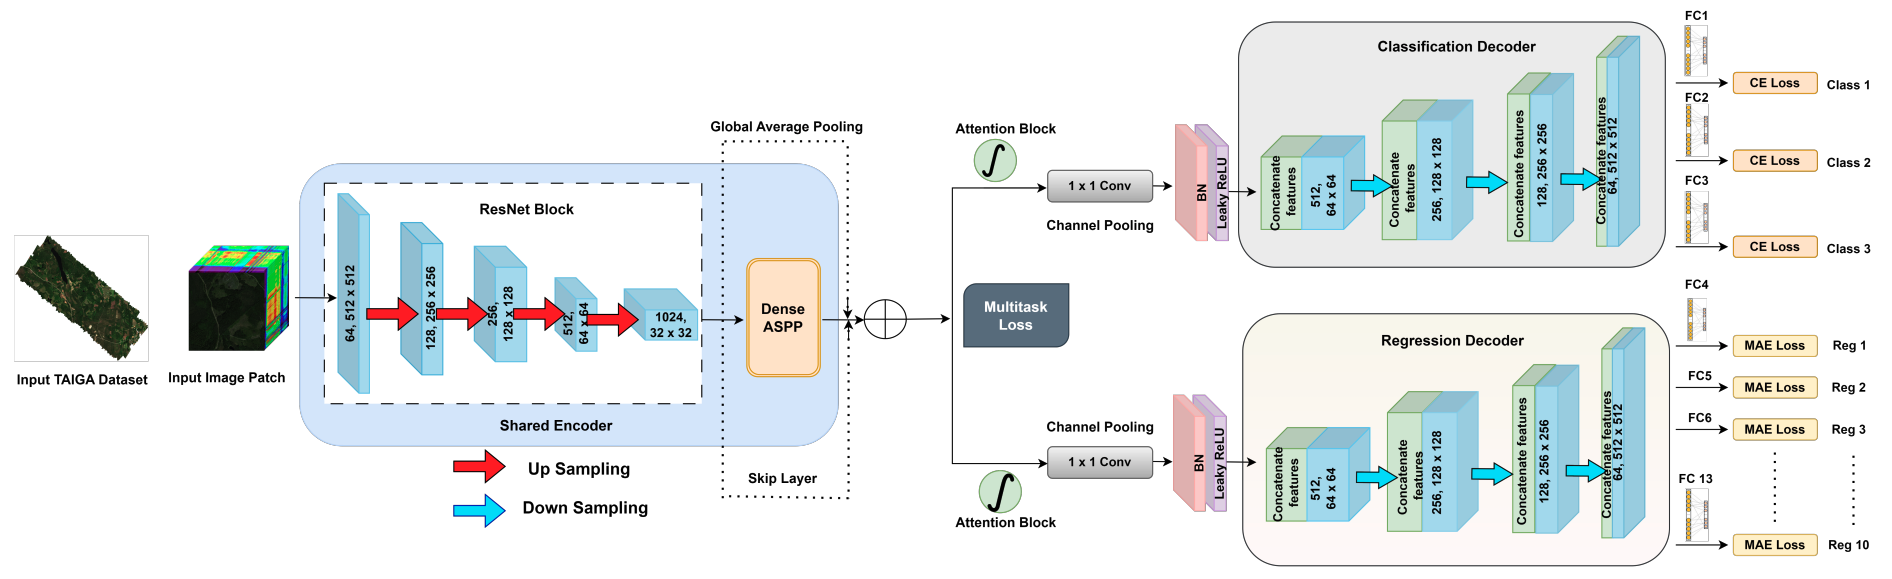
\includegraphics[width=0.95\textwidth]{img/mtl-rs-model.png}
\caption{Framework of the proposed multitask deep learning model for classification and regression of hyperspectral images. The architecture uses a shared encoder with ResNet and Dense ASPP, spectral-spatial attention blocks, and task-specific decoders. Each output has its own loss criterion: Cross-Entropy (CE) for classification and Mean Absolute Error (MAE) for regression. Adapted from \cite{chhapariya_multitask_2024}.}
\label{fig:mtl-rs-model}
\end{figure}

\cite{mottus_taiga_2022} presented TAIGA, a novel dataset for multitask learning of continuous and categorical forest variables from hyperspectral imagery. The dataset contains over 70 million labeled pixels with both continuous variables (tree height, stem volume, basal area) and categorical variables (tree species, forest type) derived from forest inventory data. They established baseline results using multitask models, showing that joint learning of continuous and categorical forest attributes improves prediction accuracy for both types of variables. The dataset enables investigation of how different forest parameters relate to each other through shared spectral signatures.

\cite{la_rosa_multi-task_2021} proposed a multi-task fully convolutional network for tree species mapping in dense forests using small training hyperspectral data. Their approach is particularly relevant for this thesis because it addresses the challenge of limited training data through multitask learning. The model implements a partial loss function that enables dense tree semantic labeling from sparse polygon-level annotations, and introduces a distance regression complementary task that enforces tree crown boundary constraints. By jointly learning species classification and distance-to-boundary regression, the model achieves 88.63\% average user accuracy and 88.59\% average producer accuracy for tree species classification in tropical forests. This demonstrates that auxiliary geometric tasks can substantially improve classification performance, similar to how TreeSatAI uses small patches for training. The key insight is that the complementary task provides additional supervision that helps the model learn better features for the primary species classification task, even when labeled data is limited.

\subsubsection{Motivation for Forest Parameter Extraction}

The application of multitask learning to forest parameter extraction from SAR is motivated by the physical relationships among forest attributes. Tree species identity influences growth patterns, wood density, and maximum attainable height. A spruce tree develops differently from an oak tree, and knowing the species provides prior information about expected height ranges. Canopy height correlates with stand age while also providing geometric information relevant to species discrimination. The height profile, crown shape, and canopy texture differ among species in ways that complement textural differences visible in SAR backscatter. By training a single model to predict species and height jointly, the shared encoder can learn features that capture these biophysical relationships, potentially improving predictions for both tasks.

However, multitask learning does not always improve performance. Sometimes it actually degrades results, a phenomenon known as \textit{negative transfer}. This occurs when tasks interfere with each other during training instead of helping each other. \cite{lyu_deep_2025} discuss negative transfer in the context of domain adaptation for remote sensing, noting that when source and target domains have conflicting feature distributions, transferring knowledge can degrade performance rather than improve it. The same principle applies to multitask learning. When tasks require conflicting representations in the shared encoder, joint training can hurt both tasks compared to training them separately.

For forest parameter extraction, species classification and height estimation appear related through the biophysical properties of trees, but they differ fundamentally in nature. One is a discrete classification problem, the other a continuous regression. The central question is whether these tasks share enough underlying structure to benefit from joint learning, or whether their different objectives create conflicting gradient signals that interfere with optimization. The classification task pushes the shared encoder to learn discriminative boundaries between species, which may help or hurt the regression task that needs smooth, continuous representations of height. When tasks compete for the limited capacity of the shared encoder, the model might end up performing both tasks worse than if they were learned separately.

Understanding when and why negative transfer occurs is crucial for designing effective multitask architectures. The gradient cosine similarity between tasks provides one way to detect conflicts. When gradients from different tasks point in opposite directions (negative cosine similarity), they are actively working against each other. Task balancing strategies, architectural choices about what to share, and careful monitoring of per-task performance during training all play a role in avoiding negative transfer.

Most existing multitask remote sensing studies leverage optical or hyperspectral imagery, either alone or in combination with SAR. This gap presents an opportunity to investigate whether the structural information encoded in SAR backscatter is sufficient to support multitask learning for forest attributes, whether negative transfer occurs when combining classification and regression from radar data, and how different parameter sharing strategies affect performance when working with radar data alone.

\section{Dataset Availability in Forest Monitoring}
\label{sec:datasets}

The development of deep learning models for forest monitoring is constrained by data availability. Unlike natural image datasets which contain millions of labeled examples, remote sensing datasets for forest applications are typically smaller and more specialized. This scarcity arises from the cost and difficulty of collecting ground-truth labels, as forest inventory measurements require trained personnel and often involve accessing remote locations.

Existing benchmark datasets for forest remote sensing tend to focus on single tasks. Some datasets provide multi-sensor imagery with species labels but do not include annotations for canopy height. Others offer LiDAR-derived height information but lack species-level labels, or cover only small geographic areas. This fragmentation means that a model trained for species classification on one dataset cannot easily incorporate height predictions from another, as the spatial locations, sensor configurations, and forest types differ.

\begin{table}[htbp]
\centering
\caption{Comparison of Forest Monitoring Datasets}
\label{tab:datasets}
\small
\begin{tabular}{lcccccccc}
\hline
\textbf{Dataset} & \textbf{S1} & \textbf{Species} & \textbf{Biomass} & \textbf{Height} & \textbf{GEDI} & \textbf{Location} & \textbf{Year} \\
\hline
FoMo-Bench & \checkmark & \checkmark & \checkmark & \checkmark & & Multiple & 2024 \\
BioMassters & \checkmark & & \checkmark & & & Finland & 2023 \\
TreeSatAI & \checkmark & \checkmark & & & \checkmark & Germany & 2023 \\
TomoSense & & \checkmark & \checkmark & \checkmark & & Germany & 2023 \\
I-MAESTRO & & \checkmark & & \checkmark & & France, etc. & 2023 \\
BAMFOREST & \checkmark & & & \checkmark & \checkmark & Germany & 2024 \\
NEON & & \checkmark & \checkmark & \checkmark & \checkmark & USA & 2021 \\
Afri-SAR & \checkmark & \checkmark & \checkmark & \checkmark & & Gabon & 2018 \\
TropiSAR & & & \checkmark & \checkmark & & Fr. Guiana & 2018 \\
AfriSAR (Full) & & \checkmark & \checkmark & \checkmark & & Gabon & 2018 \\
\hline
\end{tabular}
\end{table}

The TreeSatAI Benchmark Archive represents a notable contribution to this landscape. It provides over 50{,}000 image triplets (aerial, Sentinel-1, Sentinel-2) with labels for 20 European tree species derived from forest administration data in Lower Saxony, Germany. The dataset has enabled significant research on multi-sensor tree species classification using both traditional machine learning and deep learning methods. However, TreeSatAI focuses on species classification and does not include annotations for canopy height or other structural parameters, limiting its direct applicability for multitask learning research that combines classification and regression objectives. For canopy height specifically, several global and regional products have been developed. ~\cite{potapov_mapping_2021} produced a 30~m resolution global forest height map using GEDI and Landsat data with tree ensemble methods, achieving mean error of 9.1~m. ~\cite{lang_high-resolution_2023} improved upon this with a 10~m resolution global canopy height model using deep learning on Sentinel-2 and GEDI data, achieving RMSE of 7.9~m. More recently, ~\cite{tolan_very_2024} achieved sub-meter resolution canopy height maps using DiNOv2 models with high-resolution Maxar imagery and airborne LiDAR. These products provide potential sources for deriving height labels to extend species classification datasets. This situation motivates the exploration of dataset extension strategies. If canopy height estimates can be derived from auxiliary sources such as global canopy height products, regional LiDAR surveys, or forest inventory statistics, it becomes possible to augment existing species classification datasets for multitask learning. The quality and reliability of these derived labels, and their impact on multitask model performance, are important questions. By investigating how TreeSatAI can be extended with height information, this research aims to establish practical pathways for creating multitask-ready resources.

\subsubsection{Additional Datasets.} 
Several other datasets were reviewed but not selected for this study. The iMAESTRO dataset~\cite{aussenac_diameter_2023} is derived from Airborne Laser Scanning measurements combined with field inventory data and vegetation maps. It provides tree-level records with species identity, diameter, height, and position for over 42 million individual trees across three European forest regions (Bauges, Milicz, Sneznik). The dataset enables generation of pixel-level labels for genus segmentation, canopy height, and biomass. From a multitask learning perspective, the complete co-registration of all target variables makes it suitable for investigating whether biomass and height predictions benefit from shared representations, and whether genus segmentation provides useful features for structural estimation. However, it does not include Sentinel-1 SAR imagery directly, requiring separate acquisition and processing of SAR data. BioMassters \cite{andrea_nascetti_biomassters_nodate} provides Sentinel-1/2 imagery with biomass labels for Finnish forests, but does not include separate species annotations and the released GeoTIFFs have geolocation metadata removed. BAMFOREST \cite{troles_bamforests_2024} offers UAV-based tree crown segmentation with height information, though species labels are provided as broad categories (coniferous/broadleaf) rather than specific species. TomoSense \cite{tebaldini_tomosense_2023} contains multi-frequency tomographic SAR with species, biomass, and height labels, but the 3D tomographic cube format differs from conventional 2D image inputs, and existing implementations adapting this data for standard encoder-decoder architectures are limited. NEON \cite{weinstein_remote_2021} covers 47 US sites with species, biomass, and height measurements, though field surveys are conducted in 20$\times$20~m subplots within larger plots, resulting in incomplete spatial coverage relative to the airborne imagery. TropiSAR \cite{dubois-fernandez_tropisar_2012} and AfriSAR \cite{fatoyinbo_nasa_2021} provide tropical forest measurements with biomass and height at plot level, but species labels are either absent (TropiSAR) or sparsely distributed at individual tree positions within discrete plots (AfriSAR). FoMo-Bench \cite{bountos_fomo_2025} aggregates 15 datasets for forest monitoring tasks, though the heterogeneous sources have varying acquisition dates, resolutions, and annotation protocols, and published work demonstrating its use for joint species-height prediction specifically is limited.

\subsubsection{Motivation for Dataset Extension.}
The decision to extend TreeSatAI rather than create an entirely new dataset was driven by several practical considerations. First, TreeSatAI already provides high-quality species labels from official forest administration records, eliminating the need for costly field campaigns or manual annotation. Second, the benchmark's spatially distributed sampling across Lower Saxony ensures representation of diverse forest types and management practices. Third, the availability of official German LiDAR-derived elevation products (DTM and DSM) from the same geographic region enables accurate height label generation without requiring new airborne surveys.

From a scientific perspective, adding height information to TreeSatAI addresses a key gap in SAR-based forest monitoring research. While optical remote sensing benefits from well-established relationships between spectral signatures and both species composition and canopy structure, SAR backscatter patterns are more complex and less studied for joint species-height prediction. By creating a dataset that pairs SAR imagery with both categorical (species) and continuous (height) labels, this research enables investigation of whether these tasks share beneficial representations in the SAR domain, potentially improving performance on both tasks through multitask learning.

    \chapter{Methodology}
\label{chap:methodik}

This chapter describes the methods used in this research. It covers dataset construction, model architectures, and experimental design. The research investigates multitask learning (MTL) for SAR-based forest monitoring using two different datasets to address data limitations mentioned in the previous chapter. Section~\ref{sec:treesat_chm_dataset} presents the TreeSatAI-CHM dataset, which extends the existing TreeSatAI benchmark with canopy height labels derived from German LiDAR data. Section~\ref{sec:treesat_models} describes the model architectures developed for this dataset. These include MLP and U-Net baselines and a multitask architecture for joint species classification and height regression. Section~\ref{sec:imaestro_dataset} presents the iMAESTRO dataset. Section~\ref{sec:imaestro_models} describes the model architectures for this dataset, which integrate allometric constraints into the multitask learning framework.

\section{TreeSatAI-CHM Dataset}
\label{sec:treesat_chm_dataset}

The TreeSatAI benchmark~\cite{ahlswede_treesatai_2023} provides Sentinel-1 imagery with species labels for German forests. This section describes the technical process of extending the dataset with canopy height labels derived from official German LiDAR elevation products.

The study area covers Lower Saxony, Germany, where TreeSatAI~\cite{ahlswede_treesatai_2023} provides 50{,}381 image patches at \SI{60}{\meter} spatial extent. The benchmark covers 20 European tree species grouped into 15 tree genera, with species labels from forest administration records. TreeSatAI uses a spatially distributed sampling strategy across Lower Saxony, capturing diverse tree species across different forest types. For this research, only the Sentinel-1 component is used to investigate SAR-only multitask learning.

Each Sentinel-1 patch is provided at \SI{10}{\meter} resolution and contains two polarization channels. These are VV (co-polarized) and VH (cross-polarized). A third feature, the VV/VH ratio, is also provided as a polarimetric index that correlates with vegetation structure. The resulting three-band SAR input captures both backscatter intensity and polarimetric contrast.

The dataset construction proceeds in two stages. First, a canopy height model (CHM) is generated from digital terrain and surface models and aligned to the TreeSatAI patch grid. Second, the resulting height data is combined with Sentinel-1 backscatter to create input tensors. For each patch, four input bands are assembled: VV backscatter (dB), VH backscatter (dB), VV/VH ratio, and CHM (metres). The first three bands come from the TreeSatAI Sentinel-1 archive, while the fourth is the reprojected CHM. All bands are stacked into a single four-band GeoTIFF per patch.

\subsection{Canopy Height Model Generation}
\label{subsec:chm_generation}

\subsubsection{Elevation Data Sources}

\paragraph{}

For canopy height derivation, the elevation data comes from the Lower Saxony State Office for Geoinformation and Land Surveying (LGLN). LGLN products are derived from airborne LiDAR surveys, which provide higher vertical accuracy (typically 0.1 to 0.2~m RMSE) \cite{landesamt_fur_geoinformation_und_landesvermessung_niedersachsen_lgln_digitales_2025,landesamt_fur_geoinformation_und_landesvermessung_niedersachsen_lgln_digitales_2025-1} compared to spaceborne alternatives like TanDEM-X (2 to 10~m RMSE) \cite{wessel_accuracy_2018}. The \SI{1}{\meter} spatial resolution of LGLN products preserves fine-scale canopy structure that would be lost in coarser global products. The data are freely available through the LGLN open data portal. The temporal alignment between LGLN surveys (2014--2019) and TreeSatAI Sentinel-1 acquisitions (2017--2019) minimizes discrepancies from forest growth or disturbance.

The LGLN provides two products relevant to CHM derivation:

\begin{itemize}
    \item \textbf{DTM (Digital Terrain Model, DGM in German)}: A \SI{1}{\meter} resolution model of bare-earth elevation, derived from airborne LiDAR surveys conducted across Lower Saxony. The DTM represents ground surface elevation with vegetation and buildings removed through point cloud classification and filtering. The product is generated from multiple LiDAR acquisition campaigns and undergoes quality control procedures to ensure consistent vertical accuracy across the coverage area. The data are distributed in the ETRS89/UTM zone 32N coordinate reference system (EPSG:25832) with elevation values referenced to the German height reference system DHHN2016.
    \item \textbf{DSM (Digital Surface Model, DOM in German)}: A \SI{1}{\meter} resolution model of the top surface, including trees, buildings, and other above-ground objects. The DSM is derived from the same LiDAR point clouds as the DTM, but uses first-return pulses to capture the uppermost surface rather than ground-classified returns. This product preserves the canopy top structure and is particularly suitable for forestry applications where the highest vegetation points are of interest.
\end{itemize}

Both products are distributed as tiled GeoTIFF files covering Lower Saxony, with metadata indices in GeoJSON format that specify tile boundaries and download URLs. The tiles follow a regular grid pattern with consistent spatial extent, facilitating automated processing across large areas.

\subsubsection{Generation Procedure}

The canopy height model is computed as
\begin{equation}
    \operatorname{CHM} = \operatorname{DSM} - \operatorname{DTM} 
\end{equation}
This standard approach derives vegetation height from paired elevation products. The resulting CHM represents above-ground object height relative to terrain, corresponding to canopy top height for forested areas.

\paragraph{1) Tile Selection and Download}

The LGLN tile index is loaded as a GeoJSON file, and a spatial index is constructed to identify tiles intersecting each TreeSatAI patch. Of 49{,}573 total tiles, 6{,}210 intersect with TreeSatAI locations, achieving \SI{100}{\percent} coverage. Tiles are downloaded via HTTP from the LGLN open data portal.

\paragraph{2) Nodata Interpolation}

Nodata pixels in DTM or DSM propagate to the CHM output, creating gaps in the derived height model. These gaps typically arise from water bodies, steep terrain causing LiDAR occlusion, or areas excluded during quality control. To address this, nodata values are interpolated using iterative neighbourhood averaging.

The interpolation strategy balances gap-filling effectiveness with preservation of spatial structure. Simple nearest-neighbour filling would create blocky artefacts. Sophisticated geostatistical methods like kriging would be computationally expensive for the large dataset and could introduce unrealistic smoothing. The iterative neighbourhood averaging approach provides a middle ground. For each nodata pixel, the algorithm examines its eight neighbours and replaces the value with the mean of valid neighbours. This process repeats for five iterations, progressively filling gaps from the edges inward while maintaining local height gradients. The five-iteration limit was chosen empirically to fill typical gap sizes (5 to 10~m) without excessive propagation of edge values into larger voids.

\paragraph{3) CHM Computation and Quality Control}

After interpolation, the CHM is computed by subtracting DTM from DSM. To remove artefacts, negative CHM values are set to zero, and values exceeding the 95th percentile are clipped to that threshold. This removes implausible values from buildings, power lines, or interpolation errors while preserving the main distribution.

\begin{figure}[htbp]
    \centering
    
\includegraphics[width=0.8\textwidth]{dtm_dsm_chm.png}
    \caption[Example DTM, DSM, and CHM tiles for forested areas in Lower Saxony]{Example DTM, DSM, and CHM tiles for forested areas in Lower Saxony. The top row shows the Digital Terrain Model (DTM) representing bare-earth elevation, the middle row shows the Digital Surface Model (DSM) capturing the top surface including tree canopies, and the bottom row shows the derived Canopy Height Model (CHM).}
    \label{fig:dtm_dsm_chm}
\end{figure}

\paragraph{4) Reprojection and Alignment}

The CHM must be reprojected to match TreeSatAI Sentinel-1 geometry, which uses the WGS84 geographic coordinate system with \SI{10}{\meter} pixel spacing. This reprojection involves both coordinate transformation (from ETRS89/UTM to WGS84) and resampling (from \SI{1}{\meter} to \SI{10}{\meter} resolution). Most patches (\SI{87.7}{\percent}) fall within a single elevation tile, while \SI{12.3}{\percent} require mosaicking from multiple tiles.

The resampling strategy preserves canopy height information during the \num{10}$\times$ resolution reduction. Simple averaging would underestimate heights by including sub-canopy pixels. Nearest-neighbour resampling would create blocky artefacts. A two-stage approach inspired by PrediTree \cite{debary_preditree_2025} was adopted instead. First, a local maximum filter (\SI{10}{\meter} window) identifies the dominant canopy height within each target pixel. This preserves the tallest vegetation returns that correspond to canopy tops. Second, bilinear resampling smooths the maximum-filtered result. This produces spatially continuous height fields without blocky transitions. The combination retains local height maxima, which is important for canopy height characterization. 

\paragraph{5) Validation Against Global Canopy Height Products}

The derived CHM is validated against two global products: ETH Global Canopy Height~\cite{lang_high-resolution_2023} (\SI{10}{\meter} resolution from Sentinel-2 and GEDI LiDAR) and Meta Global Canopy Height~\cite{tolan_very_2024} (\SI{1}{\meter} resolution from Maxar imagery and airborne LiDAR). Comparisons use random pixel samples from overlapping areas.

\begin{figure}[htbp]
    \centering
    
\includegraphics[width=0.49\textwidth]{chm_lgln_meta.png}
    \hfill
    
\includegraphics[width=0.49\textwidth]{chm_lgln_eth.png}
    \caption[Validation of derived CHM against global canopy height products]{Validation of derived CHM against global canopy height products. Left: Comparison with Meta Global Canopy Height at \SI{1}{\meter} resolution. Right: Comparison with ETH Global Canopy Height at \SI{10}{\meter} resolution. Four representative tiles show side-by-side comparisons demonstrating spatial alignment and similar height patterns.}
    \label{fig:chm_validation}
\end{figure}

Visual inspection shows that the LGLN-derived CHM matches well with global products in terms of spatial alignment and height patterns. The average differences of several meters in RMSE could be due to timing differences, sensor variations, or actual uncertainty. Global products report RMSE values between 5 to 10~m when compared to airborne LiDAR \cite{lang_high-resolution_2023,tolan_very_2024}, indicating that the observed differences are within expected ranges. The LGLN-derived CHM is used as the height reference, acknowledging that the labels have some inherent uncertainty.

\subsection{Data Preprocessing}
\label{subsec:treesat_preprocessing}

With CHM patches aligned to the TreeSatAI grid, the height data are combined with Sentinel-1 backscatter to create input tensors. For each patch, four input bands are assembled: VV backscatter (dB), VH backscatter (dB), VV/VH ratio, and CHM (metres). The first three bands come from the TreeSatAI Sentinel-1 archive, while the fourth is the reprojected CHM. All bands are stacked into a single four-band GeoTIFF per patch.

\begin{figure}[htbp]
    \centering
    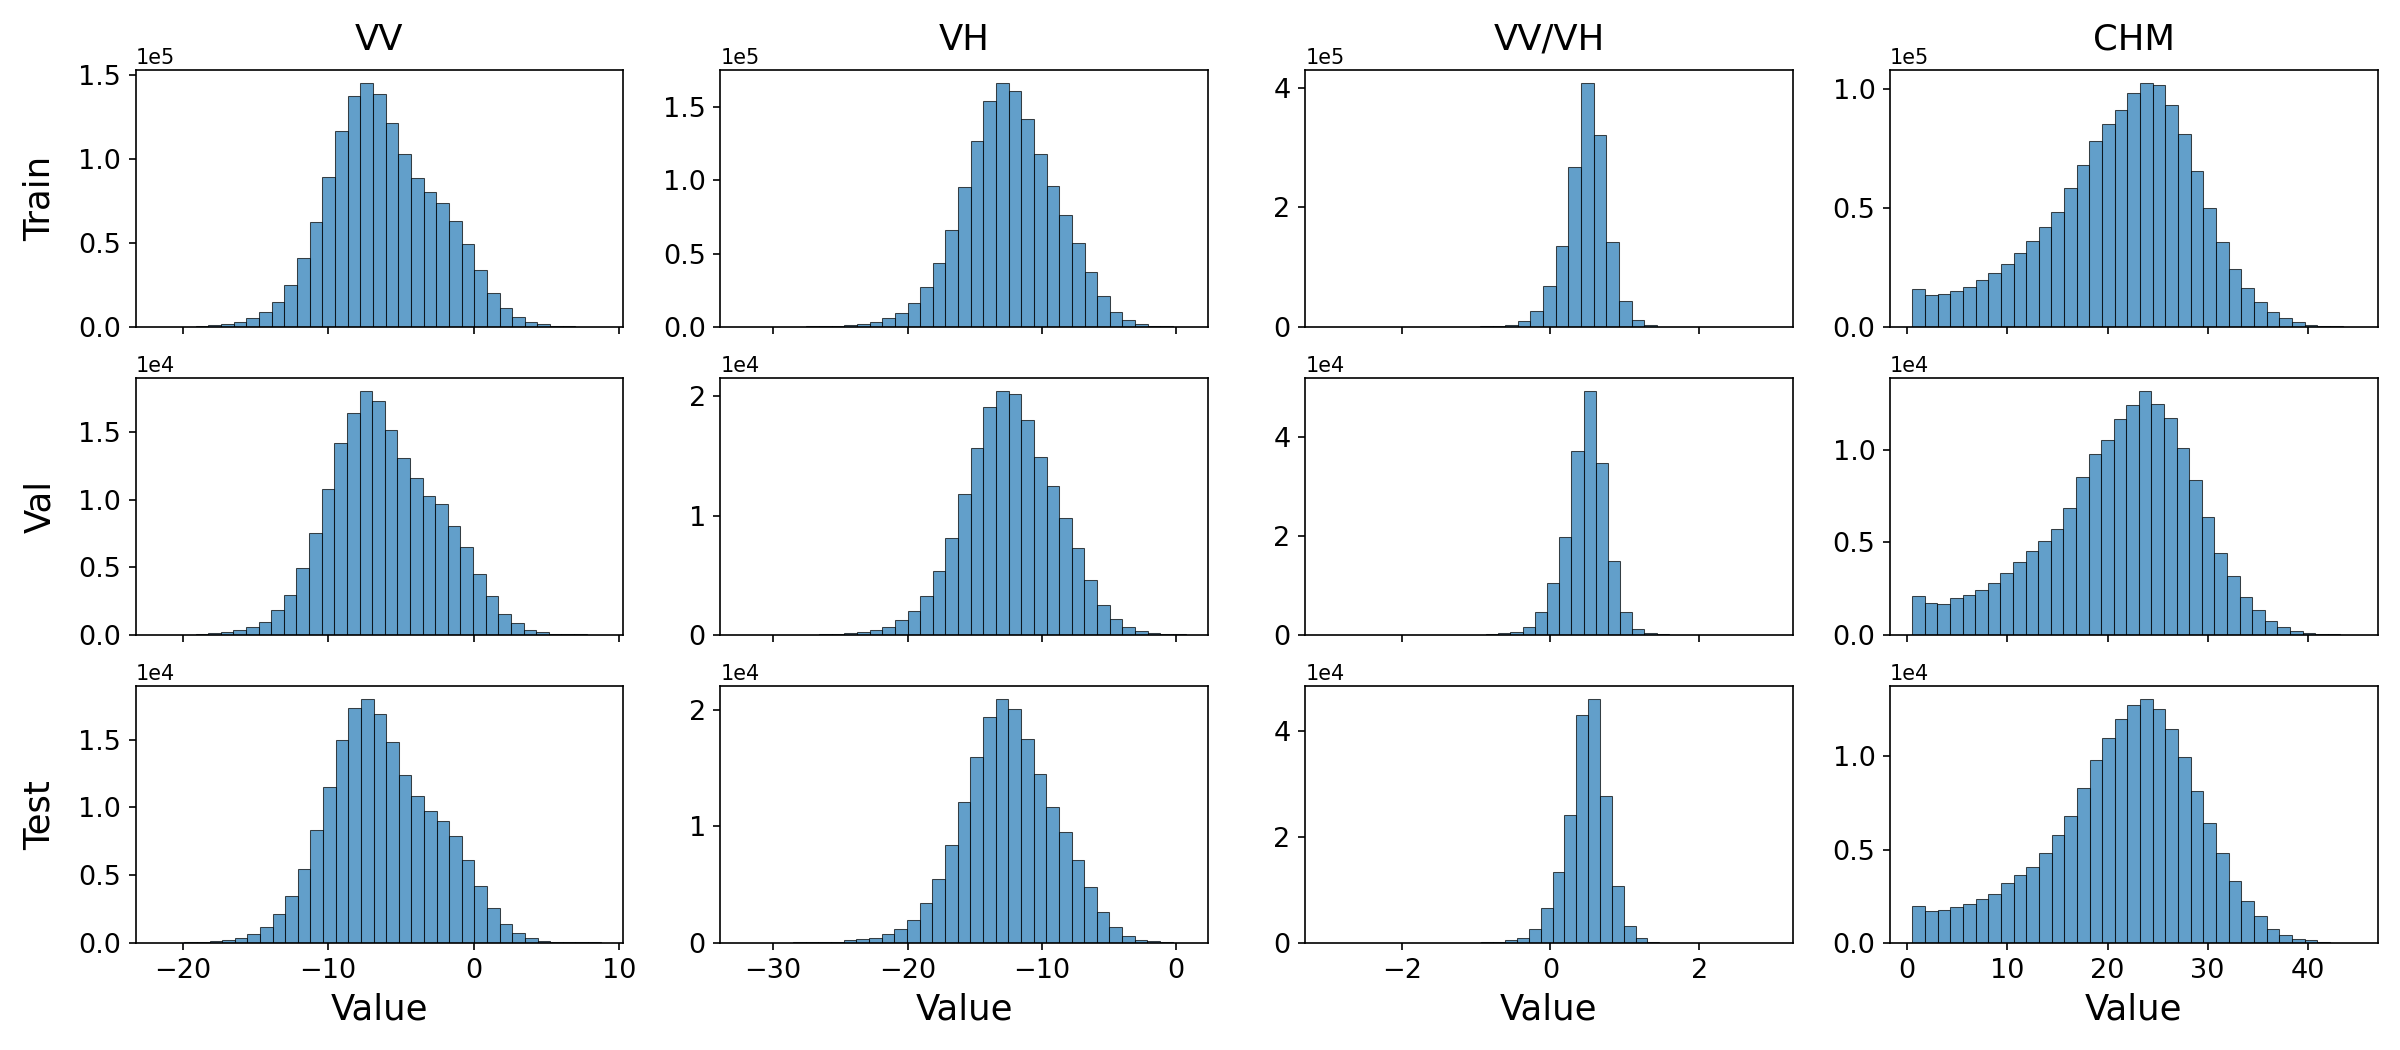
\includegraphics[width=0.9\textwidth]{histograms_train_val_test60m.png}
    \caption[Distribution of input bands across training, validation, and test splits]{Distribution of input bands across training, validation, and test splits. Each row shows histograms for one split (Train, Val, Test), with columns displaying the four input bands (VV, VH, VV/VH, CHM). The distributions are similar across splits, indicating successful stratified sampling.}
    \label{fig:histograms_splits}
\end{figure}

\subsubsection{1) Label Filtering}

Labels are filtered based on area fraction according to the TreeSatAI GitHub scripts. Only genera occupying more than \SI{7}{\percent} of patch area are retained, corresponding to approximately \SI{250}{\square\meter} coverage. This threshold addresses a fundamental challenge in multi-label classification. The challenge is how to handle species that occupy only a few pixels within a patch.

This indicates that very small area fractions often represent isolated trees or edge effects rather than meaningful forest composition, and their SAR signatures may be overwhelmed by the dominant species. The resulting filtered dataset retains multi-label complexity (average \num{2.3} genera per patch) while removing spurious labels.

\subsubsection{2) Data Splitting Strategy}

The original TreeSatAI 9:1 train:test split is retained for benchmark comparability, allowing direct comparison with published results. Within the training dataset, stratified sampling creates a validation set with 8:1:1 split ratio of train/val/test. For each patch, the primary label (genus with largest area fraction) determines the stratification. Within each genus stratification group, one ninth of samples are randomly assigned to validation, ensuring all genera are represented in both training and validation splits. This stratification is critical for rare genera, which prevent random splitting from placing all samples of uncommon species in the training set.

A limitation of this approach is that there is no spatial separation between splits. Because nearby samples share similar environmental conditions, management history, and SAR acquisition geometry, they tend to be more similar than distant samples. This spatial autocorrelation may cause performance estimates to be higher than what would be achieved on truly independent data. Additionally, TreeSatAI patches are extracted with slight spatial overlap between neighbouring locations, which further increases the similarity between samples that may end up in different splits.

Ideally, train, validation, and test sets would come from separate geographic regions. However, this is difficult for TreeSatAI because the patches are scattered across Lower Saxony rather than forming continuous areas. Creating spatial separation would require buffer zones of 5 to 10~km between splits, which would greatly reduce the usable data. Another problem is that rare genera tend to occur in specific areas (for example, \textit{Larix} is found mainly in mountainous regions). Spatial blocking could put all samples of certain species into just one split, making it impossible to train or evaluate on those species. The stratified random split is a practical choice that keeps class balance and includes rare species in all splits, even though it does not ensure spatial independence.

\begin{figure}[htbp]
    \centering
    
\includegraphics[width=0.9\textwidth]{class_distribution_60m.png}
    \caption[Distribution of patches across genera for training, validation, and test splits]{Distribution of patches across genera for training, validation, and test splits. The bar chart shows patch counts for each genus across the three splits. Picea and Pinus dominate the dataset, while several genera have fewer than 1000 patches. The stratified sampling preserves class proportions across splits, ensuring all genera are represented in training, validation, and test sets.}
    \label{fig:class_distribution_60m}
\end{figure}

\subsubsection{3) Class Weighting}

Tree species are not evenly distributed in the dataset. Common genera like \textit{Picea} and \textit{Pinus} possess many patches, while rare genera like \textit{Larix} and \textit{Betula} have fewer than 500 patches. This creates a problem for multi-label classification. Without correction, models focus on common classes and ignore rare ones because the loss from rare classes is very small.

To address this, inverse frequency weighting is adopted. For a dataset with $N$ total samples and $n_c$ samples of class $c$, the weight is
\begin{equation}
    w_c = \frac{N}{C \cdot n_c},
\end{equation}
where $C$ is the number of classes. This gives higher importance to rare classes during training. When the model misclassifies a rare genus, it contributes more to the loss than when it misclassifies a common genus. Dividing by $C$ keeps the total of all weights proportional to the dataset size, which prevents the loss from becoming too large.

Alternative weighting schemes were considered. Effective number weighting~\cite{cui_class-balanced_2019} and focal loss~\cite{lin_focal_2017} are popular options, but inverse frequency weighting was chosen because it is simple and easy to interpret. The weight scales linearly with class frequency, which makes the behaviour predictable. More complex schemes add extra hyperparameters that need tuning.

The final preprocessing converts GeoTIFF stacks and labels into arrays for deep learning. For each split, 4-band patches are stacked into tensors of shape $({N}, 4, 6, 6)$. Labels are converted to multi-hot vectors. The resulting arrays, class weights, and genus mappings are stored for model training.

\begin{figure}[htbp]
    \centering
    
\includegraphics[width=0.8\textwidth]{sample_grid_60m.png}
    \caption[Example patches from training, validation, and test sets]{Example patches from training, validation, and test sets. Each row shows randomly selected patches from one split, with columns displaying the four input bands (VV, VH, VV/VH, CHM).}
    \label{fig:sample_grid_60m}
\end{figure}

\begin{figure}[htbp]
    \centering
    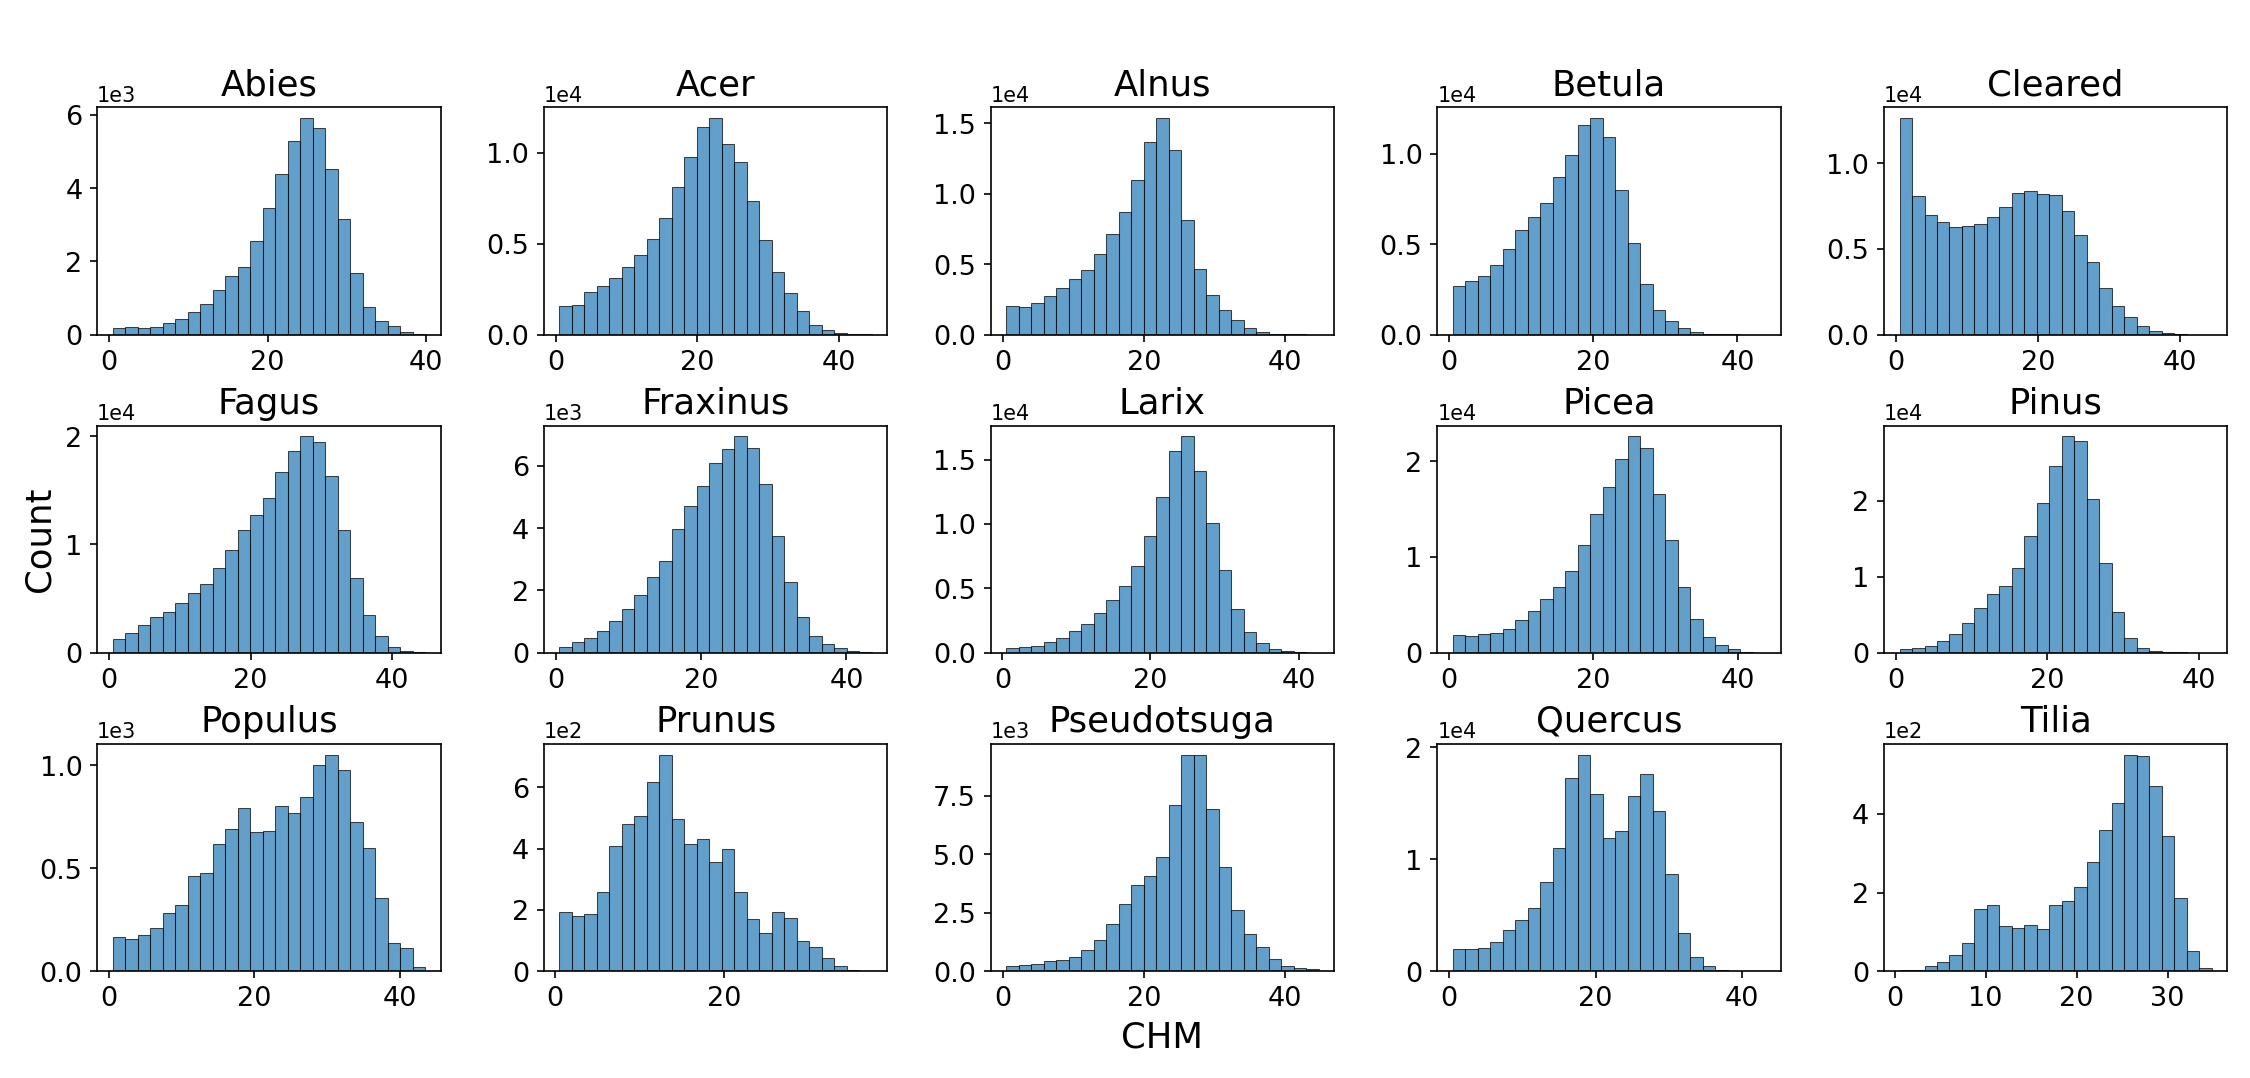
\includegraphics[width=0.9\textwidth]{chm_histograms_by_class_train_val_test_60m.png}
    \caption[CHM value distributions by genus across all splits]{CHM value distributions by genus across all splits. Each panel shows the CHM histogram for one genus. Different genera exhibit slightly different height patterns, with coniferous genera like Picea and Pinus showing taller canopies, while some broadleaf genera show lower average heights.}
    \label{fig:chm_histograms_by_class}
\end{figure}

\section{Model Architectures for TreeSatAI-CHM}
\label{sec:treesat_models}

This section describes the model architectures developed for the TreeSatAI-CHM dataset. Two categories of baseline models are used to establish reference performance: multilayer perceptrons (MLPs) following the original TreeSatAI benchmark, and U-Net architectures suitable for extension to multitask learning.

The choice of model architectures was guided by three considerations. First, the small patch size ($6 \times 6$ pixels) constrains the architectural depth. Excessive downsampling would eliminate spatial structure entirely. Second, the classification and regression tasks require architectures that can handle both discrete and continuous outputs. Third, the goal of multitask learning requires architectures with clear separation between shared and task-specific components.

MLPs serve as a simple baseline that treats each patch as a feature vector, ignoring spatial structure. This provides a lower bound on performance and enables comparison with the original TreeSatAI benchmark. In contrast, U-Nets preserve spatial information through skip connections and are naturally suited to multitask extension through shared encoders and task-specific decoders. By comparing MLP and U-Net baselines, the experiments can quantify architecture differences in performance for these tasks.

\subsection{Baseline Models}

\subsubsection{Multilayer Perceptron Baseline}

The MLP baseline follows the TreeSatAI benchmark architecture to ensure comparability with published results. \textbf{The classification MLP} receives the flattened input tensor (3 channels $\times 6 \times 6 = 108$ features) and processes it through three hidden layers of 512 units each before producing class logits for 15 genera.

The three-layer architecture with 512 units per layer was chosen based on the TreeSatAI benchmark. This capacity is sufficient for the classification task without overfitting. Each hidden layer follows the pattern Linear~$\rightarrow$~BatchNorm~$\rightarrow$~ReLU~$\rightarrow$~Dropout. Batch normalization stabilizes training by normalizing activations. Dropout provides regularization by randomly disabling units during training. The output layer produces raw logits passed through a sigmoid function for multi-label classification. A threshold of 0.5, also adapted from TreeSatAI benchmark, is applied to convert probabilities to binary predictions.

\textbf{The regression MLP} shares the same hidden layer structure but outputs a vector of length 36, reshaped to a spatial map of shape $(1, 6, 6)$. This design choice maintains the spatial output format required for height prediction while using the same feature extraction pathway as classification. To ensure non-negative height predictions (negative heights are physically meaningless) and smooth gradients near zero, the output passes through a softplus activation function

\begin{equation}
    \operatorname{softplus}(x) = \log\bigl(1 + \exp(x)\bigr).
\end{equation}

\subsubsection{U-Net Baseline}

The U-Net architecture~\cite{ronneberger_u-net_2015} uses skip connections between encoder and decoder stages to preserve spatial information during downsampling. However, for the small patch sizes ($6 \times 6$ pixels), standard U-Net architectures with multiple downsampling stages would eliminate spatial structure entirely. The encoder therefore uses only two downsampling stages. It reduces the input from $6 \times 6$ to $3 \times 3$, then to a $1 \times 1$ bottleneck. This minimal depth preserves spatial structure while allowing abstract representations.

The U-Net implementation uses three building blocks designed for efficiency and stability. \textbf{DoubleConv blocks} apply two consecutive $3 \times 3$ convolutions with batch normalization and ReLU activation. The double convolution increases the receptive field while maintaining spatial resolution. Batch normalization ensures stable gradient flow. \textbf{Down blocks} use strided convolutions (stride~2) for learnable downsampling, allowing the network to learn optimal downsampling filters. \textbf{Up blocks} use transposed convolutions for upsampling. They concatenate features with corresponding encoder skip connections to recover spatial details lost during downsampling.

\textbf{The classification U-Net} follows the encoder pathway to extract hierarchical features. After the bottleneck, the decoder reconstructs a feature map at original resolution. A $1 \times 1$ convolution produces per-pixel class activations. Global average pooling across spatial dimensions yields patch-level logits for 15 genera. This design allows the network to learn spatially-varying class probabilities before aggregating to patch-level predictions. This can capture within-patch species heterogeneity. Dropout is applied after the first upsampling stage to prevent overfitting on the relatively small dataset.

\textbf{The regression U-Net} requires full spatial output to predict height at each pixel location. The encoder progressively compresses spatial dimensions ($6\times 6 \rightarrow 3\times 3 \rightarrow 1\times 1$) while expanding feature depth ($3 \rightarrow B \rightarrow 2B \rightarrow 4B$ channels, where $B$ is the base channel count). As spatial resolution decreases, feature channels increase to maintain representational capacity. The decoder mirrors the encoder, restoring spatial resolution through skip connections. The concatenation at each decoder stage combines contextual information from deeper layers with high-resolution spatial details from the encoder. Deeper layers capture large-scale patterns while the encoder preserves fine-scale structure. This multi-scale fusion is critical for accurate height prediction. Canopy height exhibits both local variation (tree crowns) and broader patterns (stand-level structure). A final $1 \times 1$ convolution produces a single-channel output of shape $(1, 6, 6)$. This is passed through softplus activation to ensure non-negative height predictions.

The baseline models are designed with multitask learning extension in mind. The U-Net architecture is particularly suitable for this purpose because the encoder naturally provides shared representations that can serve multiple decoder heads. In subsequent experiments, a multitask U-Net variant shares the encoder while maintaining separate architectures for classification and regression decoders.

\subsection{Multitask Learning Architecture}

The multitask architecture follows the hard parameter sharing paradigm(shared encoders), which has been shown to provide effective regularisation by forcing the encoder to learn representations useful for multiple tasks~\cite{vandenhende_multi-task_2021}. A shared encoder extracts common feature representations processed by task-specific decoder heads, and enables investigation of whether species classification and height regression benefit from common SAR feature representations. This design choice was motivated by 2 factors. First, hard parameter sharing provides implicit regularization by constraining the encoder to learn representations useful for multiple objectives. This can improve generalization compared to single-task models. Second, sharing the encoder reduces the total parameter count compared to training separate models, improving computational efficiency. 

Alternative multitask architectures were considered, including soft parameter sharing (separate encoders with cross-task regularization) and task-specific adapters. However, hard parameter sharing was chosen for its simplicity and proven effectiveness in computer vision tasks. The key question is whether the two tasks are sufficiently related to benefit from shared representations, which the experiments aim to answer.

\subsubsection{Architecture Design}

The MultiTaskUNet extends the U-Net regressor baseline with an additional classification head. The shared encoder processes input through two downsampling stages ($6\times 6 \rightarrow 3\times 3 \rightarrow 1\times 1$), which learns features that must support both tasks. The classification head applies global average pooling on bottleneck features, that produces a vector passed through a fully connected layer to generate class logits. This design leverages the most abstract representation (the bottleneck) for classification and this thesis proposes that species features are best captured by high-level semantic features.

\begin{figure}[htbp]
    \centering
    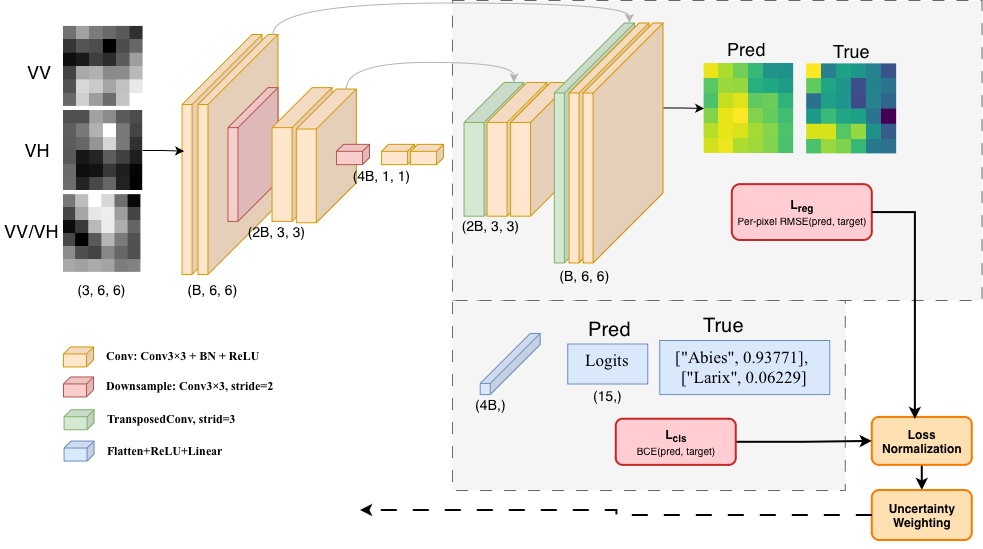
\includegraphics[width=0.95\textwidth]{treesat-model.png}
    \caption[TreeSatAI-CHM multitask learning architecture]{TreeSatAI-CHM multitask learning architecture. The model uses a shared U-Net encoder with two downsampling stages to extract features from $6\times 6$ SAR patches. Two task-specific decoder heads predict genus classification (via global average pooling and fully connected layers) and canopy height regression (via upsampling and skip connections). The shared encoder learns representations beneficial for both tasks while task-specific heads allow specialized feature refinement.}
    \label{fig:treesat_mtl_architecture}
\end{figure}

The regression decoder uses transposed convolutions and skip connections to restore spatial resolution ($1\times 1 \rightarrow 3\times 3 \rightarrow 6\times 6$). Then, a final $1\times 1$ convolution produces single-channel height predictions through softplus activation. This asymmetric design makes sense given the different task requirements, that classification needs global context since species features apply to the whole patch and regression needs spatial detail since height varies pixel to pixel. Branching classification from the bottleneck while regression uses the full decoder lets the architecture handle both needs.

\subsubsection{Loss Function Design}

\subparagraph{Loss Normalisation}

Training a multitask model requires combining multiple loss functions. This poses a fundamental challenge of loss scale mismatch, that the classification and regression tasks produce losses with different scales and units. Binary cross-entropy for classification typically ranges from 0.1 to 1.0, while RMSE for regression can range from 1 to 10 meters depending on prediction accuracy. Naively summing these losses would allow the larger-scale loss to dominate training. This would effectively ignore the smaller-scale task. To address this, individual task losses are normalised by their running means computed across batches:
\begin{equation}
    \tilde{L}_{\text{cls}} = \frac{L_{\text{cls}}}{\bar{L}_{\text{cls}}}, \qquad \tilde{L}_{\text{reg}} = \frac{L_{\text{reg}}}{\bar{L}_{\text{reg}}}.
\end{equation}
This normalisation brings both losses to similar unit scale and enables more balanced gradient contributions. The running mean is computed with exponential moving average (momentum 0.9), which provides stable normalisation while adapting to changing loss magnitudes during training.

\subparagraph{Task Weighting Strategies}

Fixed weight combination uses
\begin{equation}
    L_{\text{total}} = w_{\text{cls}} \cdot \tilde{L}_{\text{cls}} + w_{\text{reg}} \cdot \tilde{L}_{\text{reg}},
\end{equation}
where $w_{\text{cls}}$ and $w_{\text{reg}}$ are hyperparameters that control the relative importance of each task. Although this approach is simple and interpretable, it requires manual tuning to find optimal weights. Grid search over weight combinations is computationally expensive and optimal weights may vary across datasets or training stages.

An alternative approach learns task weights automatically by modelling homoscedastic uncertainty~\cite{kendall_multi-task_2017}. The key insight is that task-dependent uncertainty can serve as a principled basis for weighting. Tasks with higher inherent uncertainty should receive lower weights because their predictions are less reliable. The general uncertainty-weighted loss formulation for multiple tasks is:
\begin{equation}
    L_{\text{total}} = \sum_t \left( \frac{1}{2\sigma_t^2} L_t + \frac{1}{2} \log(\sigma_t^2) \right),
\end{equation}
where $L_t$ is the loss for task $t$ and $\sigma_t$ is a learnable parameter representing task uncertainty. The first term weights each task loss inversely proportional to its uncertainty, while the second term prevents trivially increasing uncertainties to minimize the loss. Each task loss is normalised by batch-wise mean loss magnitude before applying uncertainty weighting, ensuring that the learned uncertainties reflect relative task difficulty rather than absolute loss scales.

This formulation allows the model to automatically balance task contributions during training. If one task is inherently more difficult or noisy, the optimiser increases its uncertainty parameter, which reduces its influence on the shared encoder. For the TreeSatAI-CHM two-task case (classification and regression), this becomes:
\begin{equation}
    L_{\text{total}} = \frac{1}{2\sigma_{\text{cls}}^2} \tilde{L}_{\text{cls}} + \frac{1}{2} \log(\sigma_{\text{cls}}^2) + \frac{1}{2\sigma_{\text{reg}}^2} \tilde{L}_{\text{reg}} + \frac{1}{2} \log(\sigma_{\text{reg}}^2).
\end{equation}
The experiments compare both weighting schemes to determine which produces better multitask performance.

\subsubsection{Gradient Analysis}

A critical question in multitask learning is whether the tasks are compatible. Do they benefit from shared representations, or do they compete for encoder capacity? Gradient cosine similarity analysis provides insight into this question, which measures the alignment between task-specific gradients at each layer.

At each encoder layer, gradients from classification and regression losses are computed separately:
\begin{equation}
    \cos(\theta_{\text{layer}}) = \frac{\nabla_{\theta_{\text{layer}}} L_{\text{cls}} \cdot \nabla_{\theta_{\text{layer}}} L_{\text{reg}}}{\left\lVert\nabla_{\theta_{\text{layer}}} L_{\text{cls}}\right\rVert \cdot \left\lVert\nabla_{\theta_{\text{layer}}} L_{\text{reg}}\right\rVert}.
\end{equation}
Positive cosine similarity ($\cos(\theta) > 0$) indicates that both tasks benefit from similar parameter updates at that layer and suggests compatible learning objectives, while negative similarity ($\cos(\theta) < 0$) indicates gradient conflict and optimizing one task would harm the other. Zero similarity suggests independence. 

This analysis is performed at three encoder locations (enc1, enc2, bottleneck). It monitors whether tasks converge toward shared representations or compete for encoder capacity. If similarity is consistently positive across layers and training epochs, it suggests that species classification and height regression share beneficial SAR features. Instead, persistent negative similarity would indicate that the tasks are fundamentally incompatible and may not benefit from joint training. The gradient analysis provides interpretable diagnostics for understanding multitask learning dynamics.

\section{iMAESTRO Dataset}
\label{sec:imaestro_dataset}


\paragraph{Overview}

The dataset covers three European forest regions. These are Bauges (France), Milicz (Poland), and Sneznik (Slovenia), spanning over \SI{100000}{\hectare} with approximately 42 million individual trees from 51 species. The three sites were chosen to represent diverse forest types. Bauges exhibits mixed temperate mountain forests with high structural heterogeneity. Milicz represents lowland pine-oak forests characteristic of Central Europe. Sneznik contains old-growth beech-fir forests typical of the Dinaric Alps. This diversity ensures that models trained on iMAESTRO data encounter varied forest conditions, improving potential for generalization.

All structural data are organised on a \SI{25}{\meter} grid resolution, where each cell represents \SI{0.0625}{\hectare}. This resolution was chosen to match typical forest inventory plot sizes and to provide sufficient spatial detail for SAR analysis while maintaining computational tractability. The raw data for each site consist of tree-level CSV files containing individual tree attributes (cell identifier, species name, tree count, diameter at breast height, and tree height) and raster files encoding cell identifiers.

\subsection{Processing Raw iMAESTRO Data}

\subsubsection{1) Deriving Reference Labels}

Individual tree biomass is estimated using species-specific allometric equations rather than generic models. This choice reflects the substantial variation in wood properties across species. Coniferous species like \textit{Picea abies} (wood density \SI{0.43}{\gram\per\centi\meter\cubed}) produce less biomass per unit volume than hardwoods like \textit{Quercus robur} (wood density \SI{0.74}{\gram\per\centi\meter\cubed})~\cite{zanne_data_2009}. Using species-specific parameters ensures that the biomass labels accurately reflect ecological reality. This enables the multitask model to learn meaningful relationships between SAR backscatter, species composition, and biomass.

The allometric equations follow the general form
\begin{equation}
    \operatorname{Biomass}~(\si{\kilogram}) = a \times \operatorname{DBH}^b \times \operatorname{wood\_density},
\end{equation}
where $a$ and $b$ are species-specific allometric coefficients, DBH is diameter at breast height (\si{\centi\meter}), and wood density is in \si{\gram\per\centi\meter\cubed}. The power-law relationship between DBH and biomass reflects the geometric scaling of tree dimensions. As trees grow taller and wider, their volume (and thus biomass) increases faster than their diameter. The exponent $b$ typically ranges from 2.0 to 2.8 depending on species and growth form.

Parameters were compiled from published literature for 52 European temperate forest species~\cite{forrester_generalized_2017}, prioritizing studies from similar climatic regions to ensure transferability. Wood density values were obtained from the global wood density database~\cite{zanne_data_2009,chave_towards_2009}. For species without available parameters, default values were applied ($a = 0.0673$, $b = 2.5$, wood density $= 0.55$~\si{\gram\per\centi\meter\cubed}), representing average values for temperate broadleaf species. These defaults affect fewer than \SI{5}{\percent} of trees in the dataset, as most abundant species have well-established allometric relationships.

\subsubsection{2) Aggregating Cell-Level Data}

Data are aggregated to the \SI{25}{\meter} grid cell level to match the spatial resolution provided from the original dataset. This resolution represents a compromise between preserving spatial detail and ensuring sufficient samples per pixel for robust statistics. At finer resolutions (e.g., \SI{10}{\meter}), many cells would contain few or no trees, leading to noisy labels. At coarser resolutions (e.g., \SI{100}{\meter}), spatial heterogeneity would be lost, reducing the model's ability to learn fine-scale patterns.

For each cell, total biomass is computed by summing individual tree biomass weighted by count, then converted to metric tons per hectare (t/ha). This area-normalized metric is standard in forestry and enables comparison across different spatial scales. Height statistics use the 95th percentile (height95) as the primary canopy height metric. The 95th percentile was chosen over maximum height because it is less sensitive to outliers (e.g., exceptionally tall emergent trees or measurement errors) while still capturing the dominant canopy structure. This metric has been widely adopted in LiDAR-based forest monitoring and provides consistency with the TreeSatAI-CHM dataset.

Species composition is determined by identifying the dominant genus (highest tree count) within each cell, reducing 51 species to 31 genus-level categories. This aggregation was necessary for several reasons. First, many species have very few samples in the dataset, making species-level classification infeasible. Second, SAR backscatter is more sensitive to structural differences (e.g., coniferous vs. broadleaf, tree size) than to subtle species-level variations within a genus. The dominant genus approach (rather than multi-label classification) was chosen because \SI{25}{\meter} cells typically contain a single dominant genus (\SI{78}{\percent} of cells have $>$\SI{80}{\percent} of trees from one genus). Multi-label classification would add complexity without substantial benefit for this dataset.

\begin{figure}[htbp]
    \centering
    
\includegraphics[width=0.49\textwidth]{height_hist_per_genus_across_sites.png}
    \hfill
    
\includegraphics[width=0.49\textwidth]{biomass_hist_per_genus_across_sites.png}
    \caption[Distribution of biomass and height values by genus across all three sites]{Distribution of biomass and height values by genus across all three sites. Left: Biomass distributions. Right: Height distributions. \textit{Fagus} and \textit{Abies} dominate the dataset with distinct characteristics. Coniferous genera generally show higher biomass values relative to height due to higher wood density.}
    \label{fig:imaestro_biomass_height_by_genus}
\end{figure}

\begin{figure}[htbp]
    \centering
    
\includegraphics[width=0.9\textwidth]{genus_distribution.png}
    \caption[Overall genus distribution in the iMAESTRO dataset]{Overall genus distribution in the iMAESTRO dataset. The bar chart shows the total number of cells for each genus across all three study sites. \textit{Fagus} and \textit{Abies} are the most abundant genera.}
    \label{fig:imaestro_genus_distribution}
\end{figure}

\subsubsection{3) Generating Raster Data}

Cell-level statistics are converted to spatially explicit GeoTIFF rasters: biomass (t/ha), height95 (m), and dominant genus (numerical code). The raster transformation uses site-specific coordinate reference systems with consistent \SI{25}{\meter} pixel size.

When converting tree-level data to gridded rasters, the resulting maps can show abrupt jumps between neighboring cells. This happens because each cell is computed independently from the trees it contains. For example, one cell might have a few very tall trees giving it high average height, while the adjacent cell has shorter trees. Similarly, the genus map can show scattered single-cell patches where one genus appears isolated among different surrounding genera. While real forests do have natural variation, these sharp pixel-to-pixel changes can make it harder for the model to learn smooth spatial patterns from SAR data.

To address this, spatial smoothing is applied to make the maps more spatially coherent while keeping real forest patterns intact. The smoothing is intentionally gentle to avoid erasing true forest structure like edges between different stand types.

For continuous variables (biomass and height95), an outlier detection and correction approach is used. For each pixel, the method looks at its $5\times 5$ neighborhood and calculates the median absolute deviation (MAD), which measures how much values vary locally. The MAD is more reliable than standard deviation because it is not affected by a few extreme values. If a pixel's value differs from its neighborhood median by more than two standard deviations (estimated as $1.4826 \times \text{MAD}$), it is considered an outlier. Instead of fully replacing it with the neighborhood median, the pixel value is adjusted halfway toward the median. This preserves gradual changes across the landscape (like biomass increasing from young to mature forest) and keeps sharp boundaries (like forest edges) while removing isolated spikes or dips.

The $5\times 5$ window size (\SI{125}{\meter} $\times$ \SI{125}{\meter}) was chosen to match the scale of SAR backscatter patterns, which typically span multiple pixels due to the sensor's resolution and speckle characteristics.

For the categorical genus layer, a majority filter is applied. This common technique in spatial analysis replaces each pixel's genus code with the most common genus in its $5\times 5$ neighborhood. The majority filter smooths boundaries between different forest types and removes isolated single-pixel misclassifications, which are common when assigning discrete categories to continuous forest gradients. This approach is well-suited for genus classification because forests naturally show spatial clustering. Trees of the same genus tend to grow together due to similar environmental preferences and management practices.

Only pixels with valid data are modified in both smoothing operations, preserving the original spatial extent and preventing artificial expansion of the forest mask into non-forested areas.

\subsection{Processing Sentinel-1 GRD Data}

\paragraph{SAR Data Selection}

Sentinel-1 Ground Range Detected (GRD) products~\cite{torres_gmes_2012} are downloaded from the Alaska Satellite Facility. For each site, a single-date acquisition from the 2019 growing season is selected with Interferometric Wide swath mode and dual polarisation (VV and VH). The single-date approach was chosen to match the temporal snapshot nature of the iMAESTRO structural data, avoiding complications from seasonal vegetation changes or forest disturbances between acquisitions. Growing season acquisitions were prioritized because vegetation with leaves provides stronger volume scattering from forest canopies, enhancing the SAR sensitivity to forest structure.

\paragraph{Radiometric and Geometric Correction}

The GRD products are processed using ESA SNAP software, which provides standardized processing workflows for Sentinel-1 data. The processing chain applies precise orbit files (available 2--3 weeks post-acquisition) to refine satellite position and velocity, which is essential for accurate geocoding. Radiometric calibration converts digital numbers to sigma nought backscatter coefficients, which represent the radar cross-section per unit area in the slant range plane. This calibration accounts for antenna gain patterns and range spreading loss, ensuring that backscatter values are comparable across different acquisition geometries.

Terrain correction is applied using Range--Doppler orthorectification with SRTM \SI{1}{arcsecond} DEM (approximately \SI{30}{\meter} resolution). This step corrects for geometric distortions caused by topography, which can be significant in mountainous areas like Bauges and Sneznik. The terrain correction also reprojects the data from the native SAR geometry to site-specific coordinate reference systems (Lambert-93 for Bauges, PUWG 1992 for Milicz, D96/TM for Sneznik), ensuring perfect alignment with iMAESTRO structural layers.

\paragraph{Resampling and Logarithmic Scaling}

After terrain correction, SAR backscatter is resampled to the \SI{25}{\meter} grid using bilinear interpolation. This resampling averages approximately $6.25$ input pixels (\SI{10}{\meter} resolution) into each output pixel, reducing speckle noise while preserving spatial patterns. Bilinear interpolation was chosen over nearest-neighbour (which would preserve speckle) or cubic interpolation (which would be computationally expensive) as a pragmatic compromise.

Calibrated sigma nought values are converted to decibels (dB) as
\begin{equation}
    \sigma_{\text{dB}} = 10 \times \log_{10}(\sigma_{\text{linear}}).
\end{equation}
The logarithmic transformation is standard in SAR processing because backscatter values span several orders of magnitude (e.g., \numrange{0.01}{1.0} in linear units), and the dB scale compresses this range into a more manageable interval (e.g., \numrange{-20}{0}~dB) that is approximately normally distributed. The dB scale also has the advantage that multiplicative effects in the linear domain (such as attenuation) become additive in the log domain, simplifying interpretation.

Both VV and VH polarisation channels are processed and stored as separate GeoTIFF files. Pixels with invalid backscatter values (e.g., due to layover, shadow, or water bodies) are assigned a NoData value of $-9999$, enabling proper masking during subsequent patch extraction.

\subsection{Preparing Training Data}

\subsubsection{1) Multi-Channel Data Stacking}

For each site, five raster layers are stacked into a single multi-channel array: (0) VH backscatter (dB), (1) VV backscatter (dB), (2) biomass (t/ha), (3) dominant genus (numerical code), and (4) height95 (m). All layers are verified to have identical spatial dimensions and coordinate reference systems. A global valid data mask is computed to identify pixels where all five channels contain valid values, defining the usable extent of each site.

\subsubsection{2) Patch Extraction with Spatial Blocking}

A spatial blocking strategy is implemented to prevent spatial autocorrelation from inflating performance estimates. Unlike the TreeSatAI-CHM dataset (where spatial blocking was infeasible due to distributed sampling), the iMAESTRO data consist of contiguous rasters covering entire forest landscapes, making spatial blocking both possible and necessary. Without spatial separation between train and test sets, the model could exploit spatial autocorrelation to achieve artificially high performance: neighbouring patches are similar due to shared environmental conditions, and a model that memorizes training patch locations could perform well on nearby test patches without truly learning generalizable features.

Each site is divided into non-overlapping rectangular blocks (4$\times$4 patches per block), and entire blocks are assigned to train, validation, or test sets. With patch size of $64\times 64$ pixels and stride of 32 pixels (\SI{50}{\percent} overlap), each block covers \SI{3.2}{\kilo\meter} $\times$ \SI{3.2}{\kilo\meter} on the ground. This block size was chosen to be large enough to capture meaningful forest landscape patterns (multiple stands, topographic variation) while small enough to provide sufficient blocks for splitting across the three sets.

Within each block, patches are extracted using a sliding window with \SI{50}{\percent} overlap. The overlap increases the number of training samples while maintaining spatial independence between blocks (patches from different blocks never overlap). Patches are retained if at least \SI{20}{\percent} of pixels contain valid data and the dominant genus channel contains at least one valid pixel. The \SI{20}{\percent} threshold excludes patches dominated by non-forest areas (water, clearings) while retaining patches near forest edges where there should be at least partial coverage.

\subsubsection{3) Train--Validation--Test Splitting}

Blocks are randomly shuffled and sequentially assigned to train (\SI{75}{\percent}), validation (\SI{15}{\percent}), and test (\SI{10}{\percent}) sets. The assignment algorithm iteratively selects the split that is furthest below its target proportion and assigns the next block to that split, ensuring that the final proportions closely match the targets. A fixed random seed ensures reproducibility across different runs of the preprocessing pipeline.

The spatial blocking approach ensures that validation and test sets truly represent held-out geographic areas, which is critical for assessing generalisation to new locations. The validation set enables hyperparameter tuning and early stopping without contaminating the test set, while the test set provides an unbiased estimate of generalization performance.

Final training data are exported as NumPy arrays in \texttt{.npy} format. For each split, three files are created: patches (4D array of shape $N\times 5\times 64\times 64$), \texttt{labels\_dominant\_genus} (1D array), and \texttt{sites} (1D array). Biomass and height95 values are embedded in channels~2 and~4 of the patch arrays.

\paragraph{Trade-offs and Limitations}

The random block assignment ensures geographic diversity in each split, that all three splits contain blocks from different parts of each landscape, preventing site-specific biases. However, this approach does not guarantee balanced genus distributions across splits, as some genera may be concentrated in specific regions. Empirical analysis confirmed that all major genera (\textit{Fagus}, \textit{Abies}, \textit{Pinus}, \textit{Picea}, \textit{Quercus}, \textit{Fraxinus}) are represented in all three splits, though proportions vary slightly.

\begin{figure}[htbp]
    \centering
    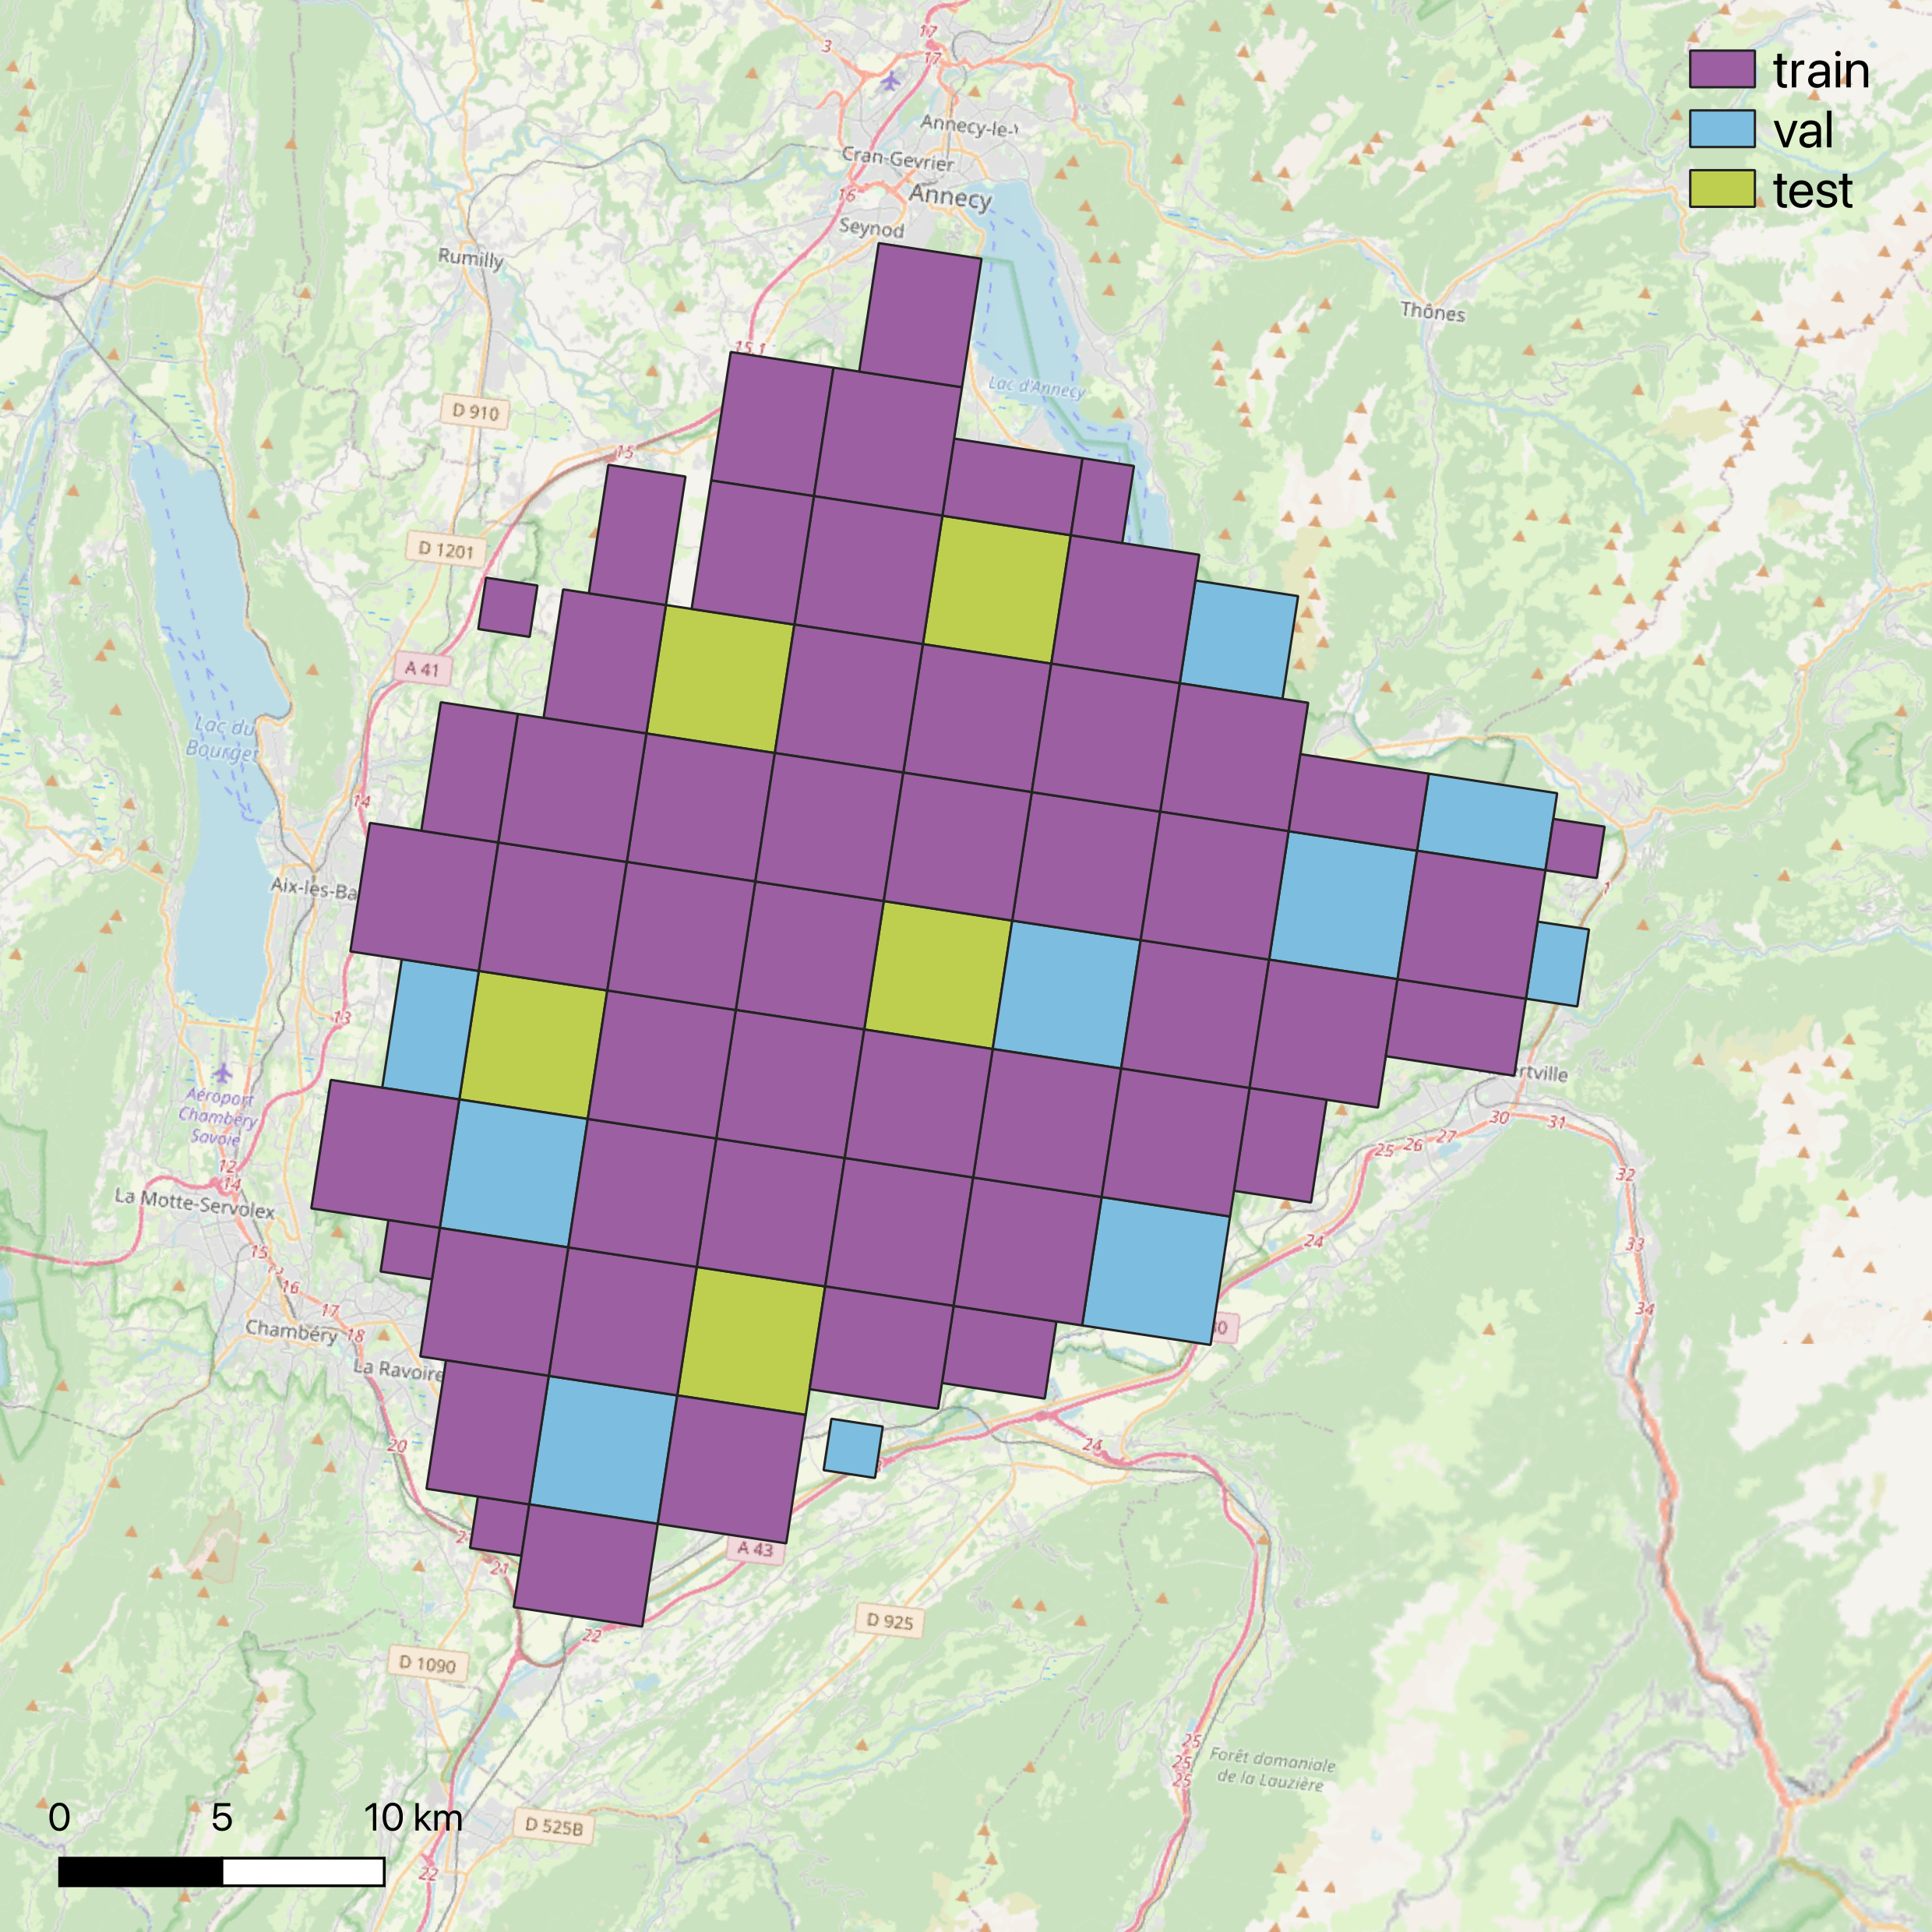
\includegraphics[width=0.32\textwidth]{bauges_blocks.png}
    \hfill
    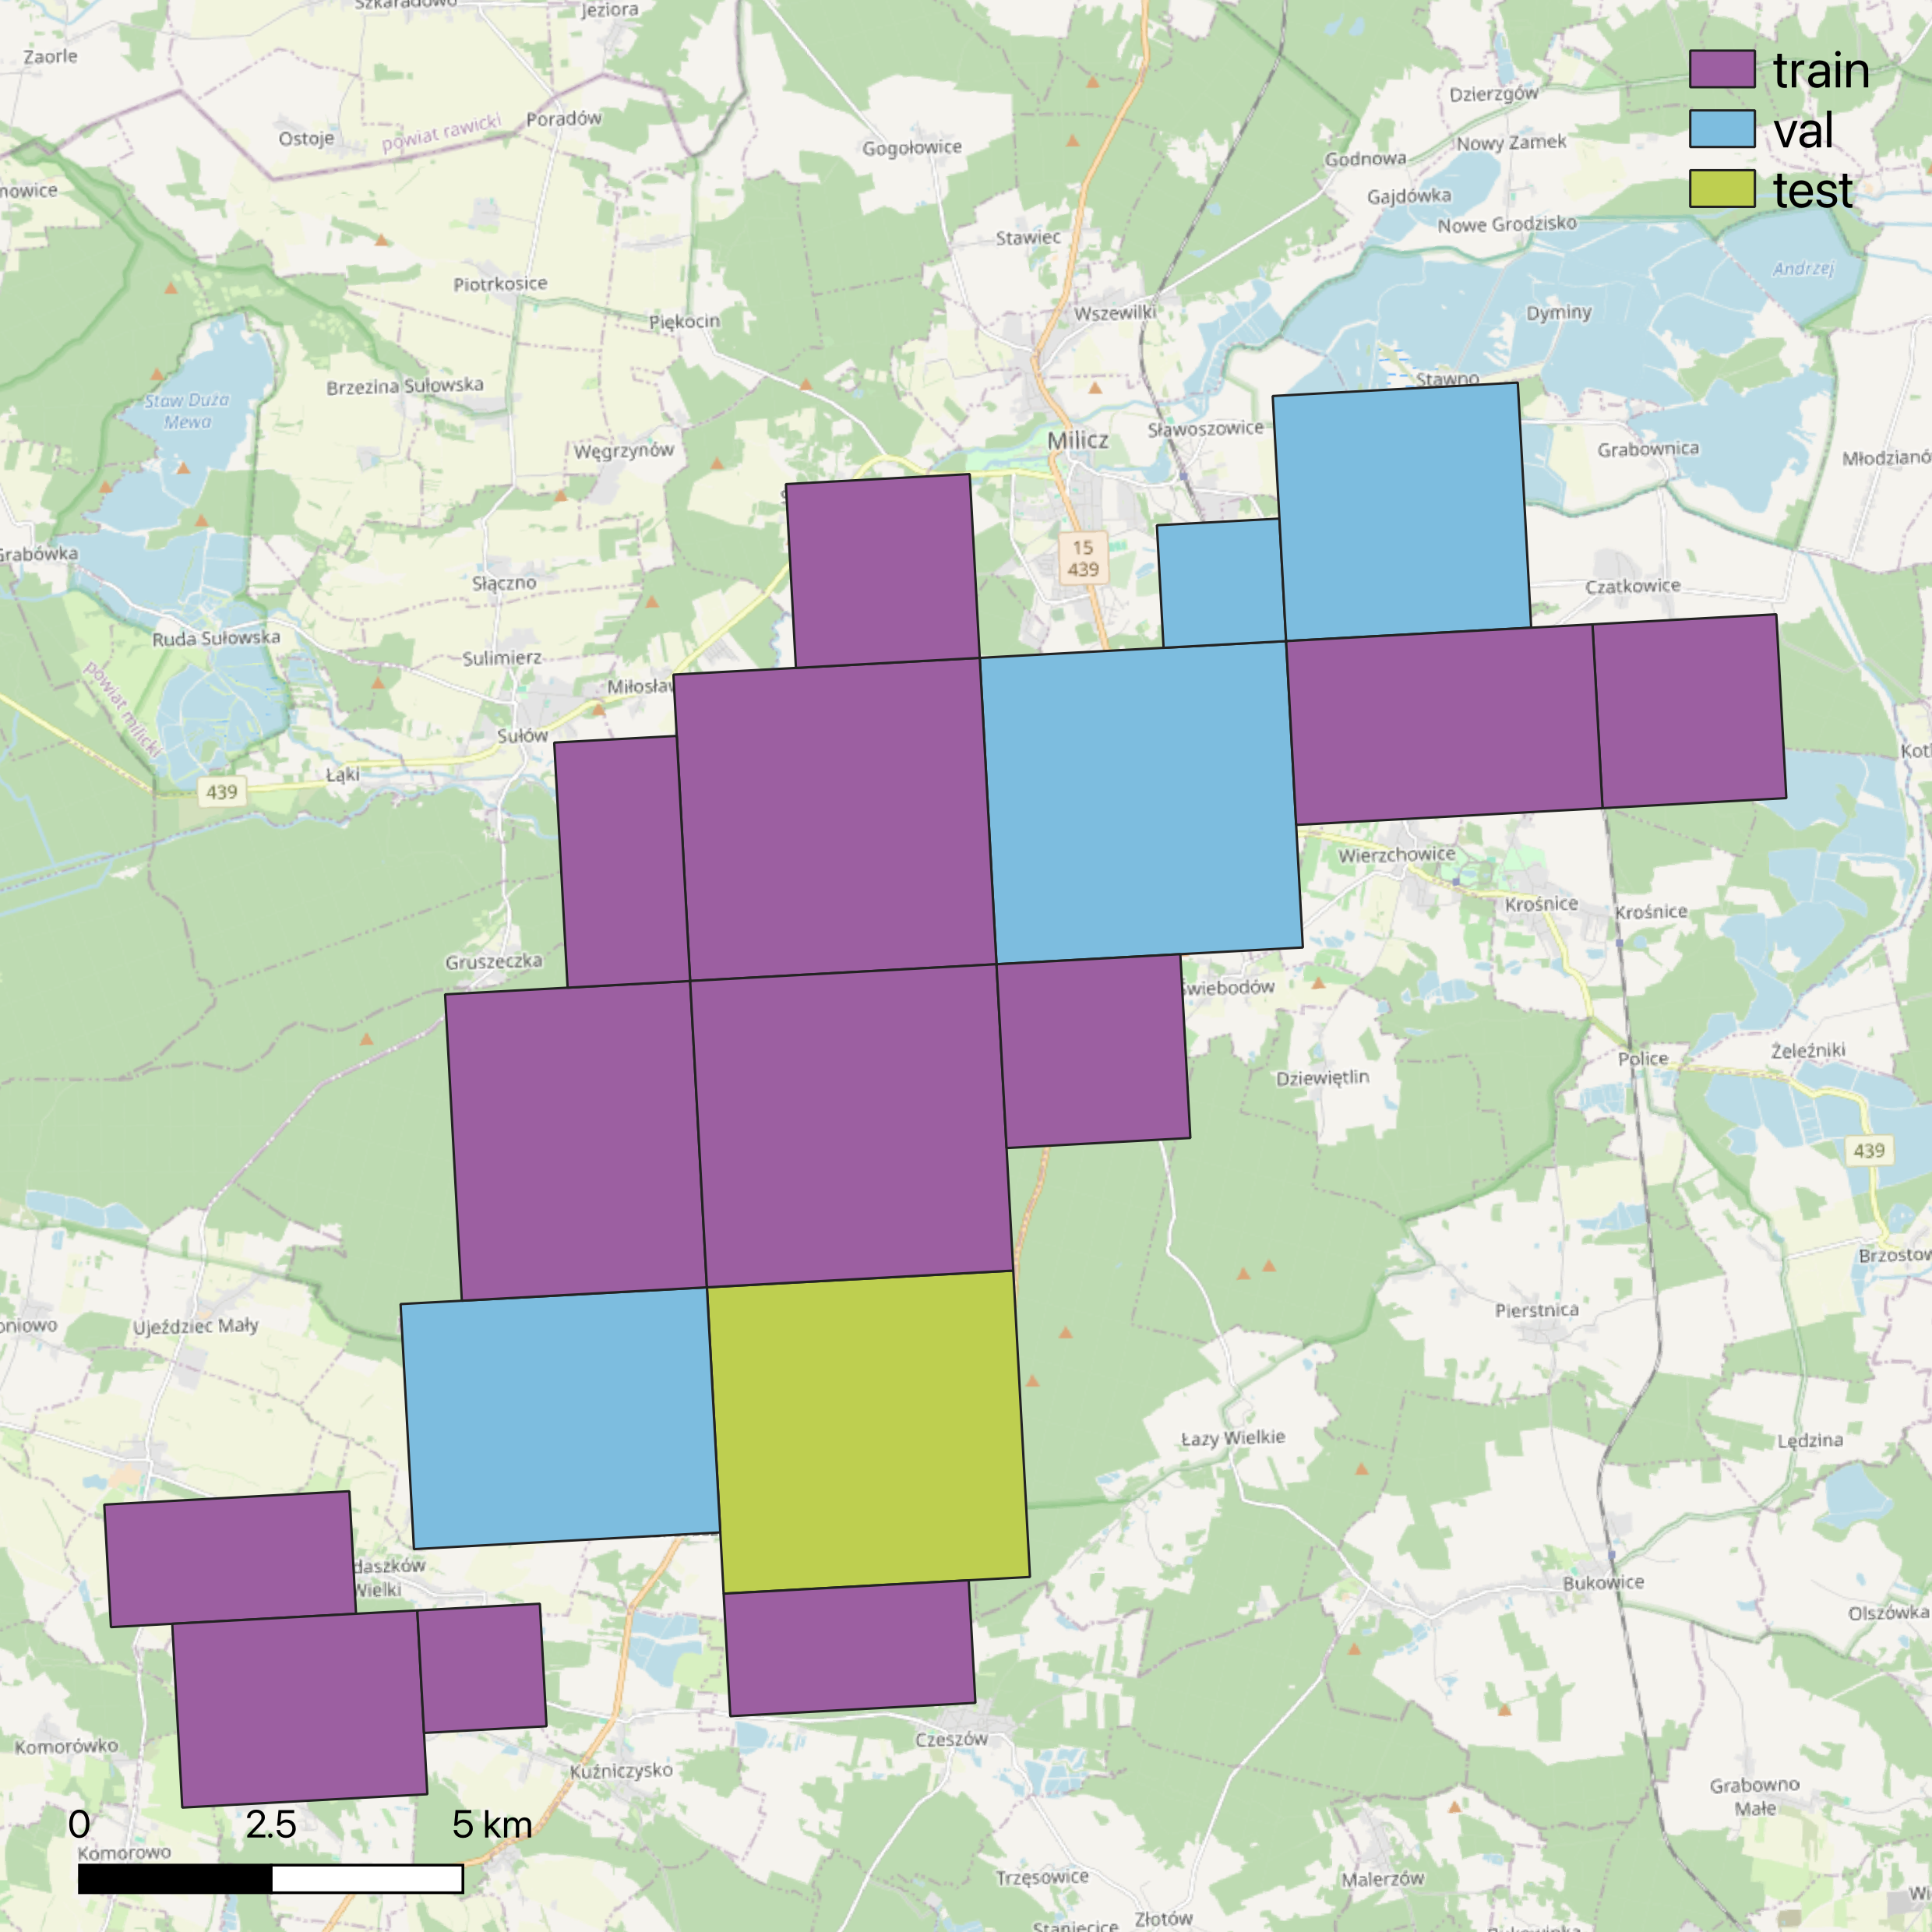
\includegraphics[width=0.32\textwidth]{milicz_blocks.png}
    \hfill
    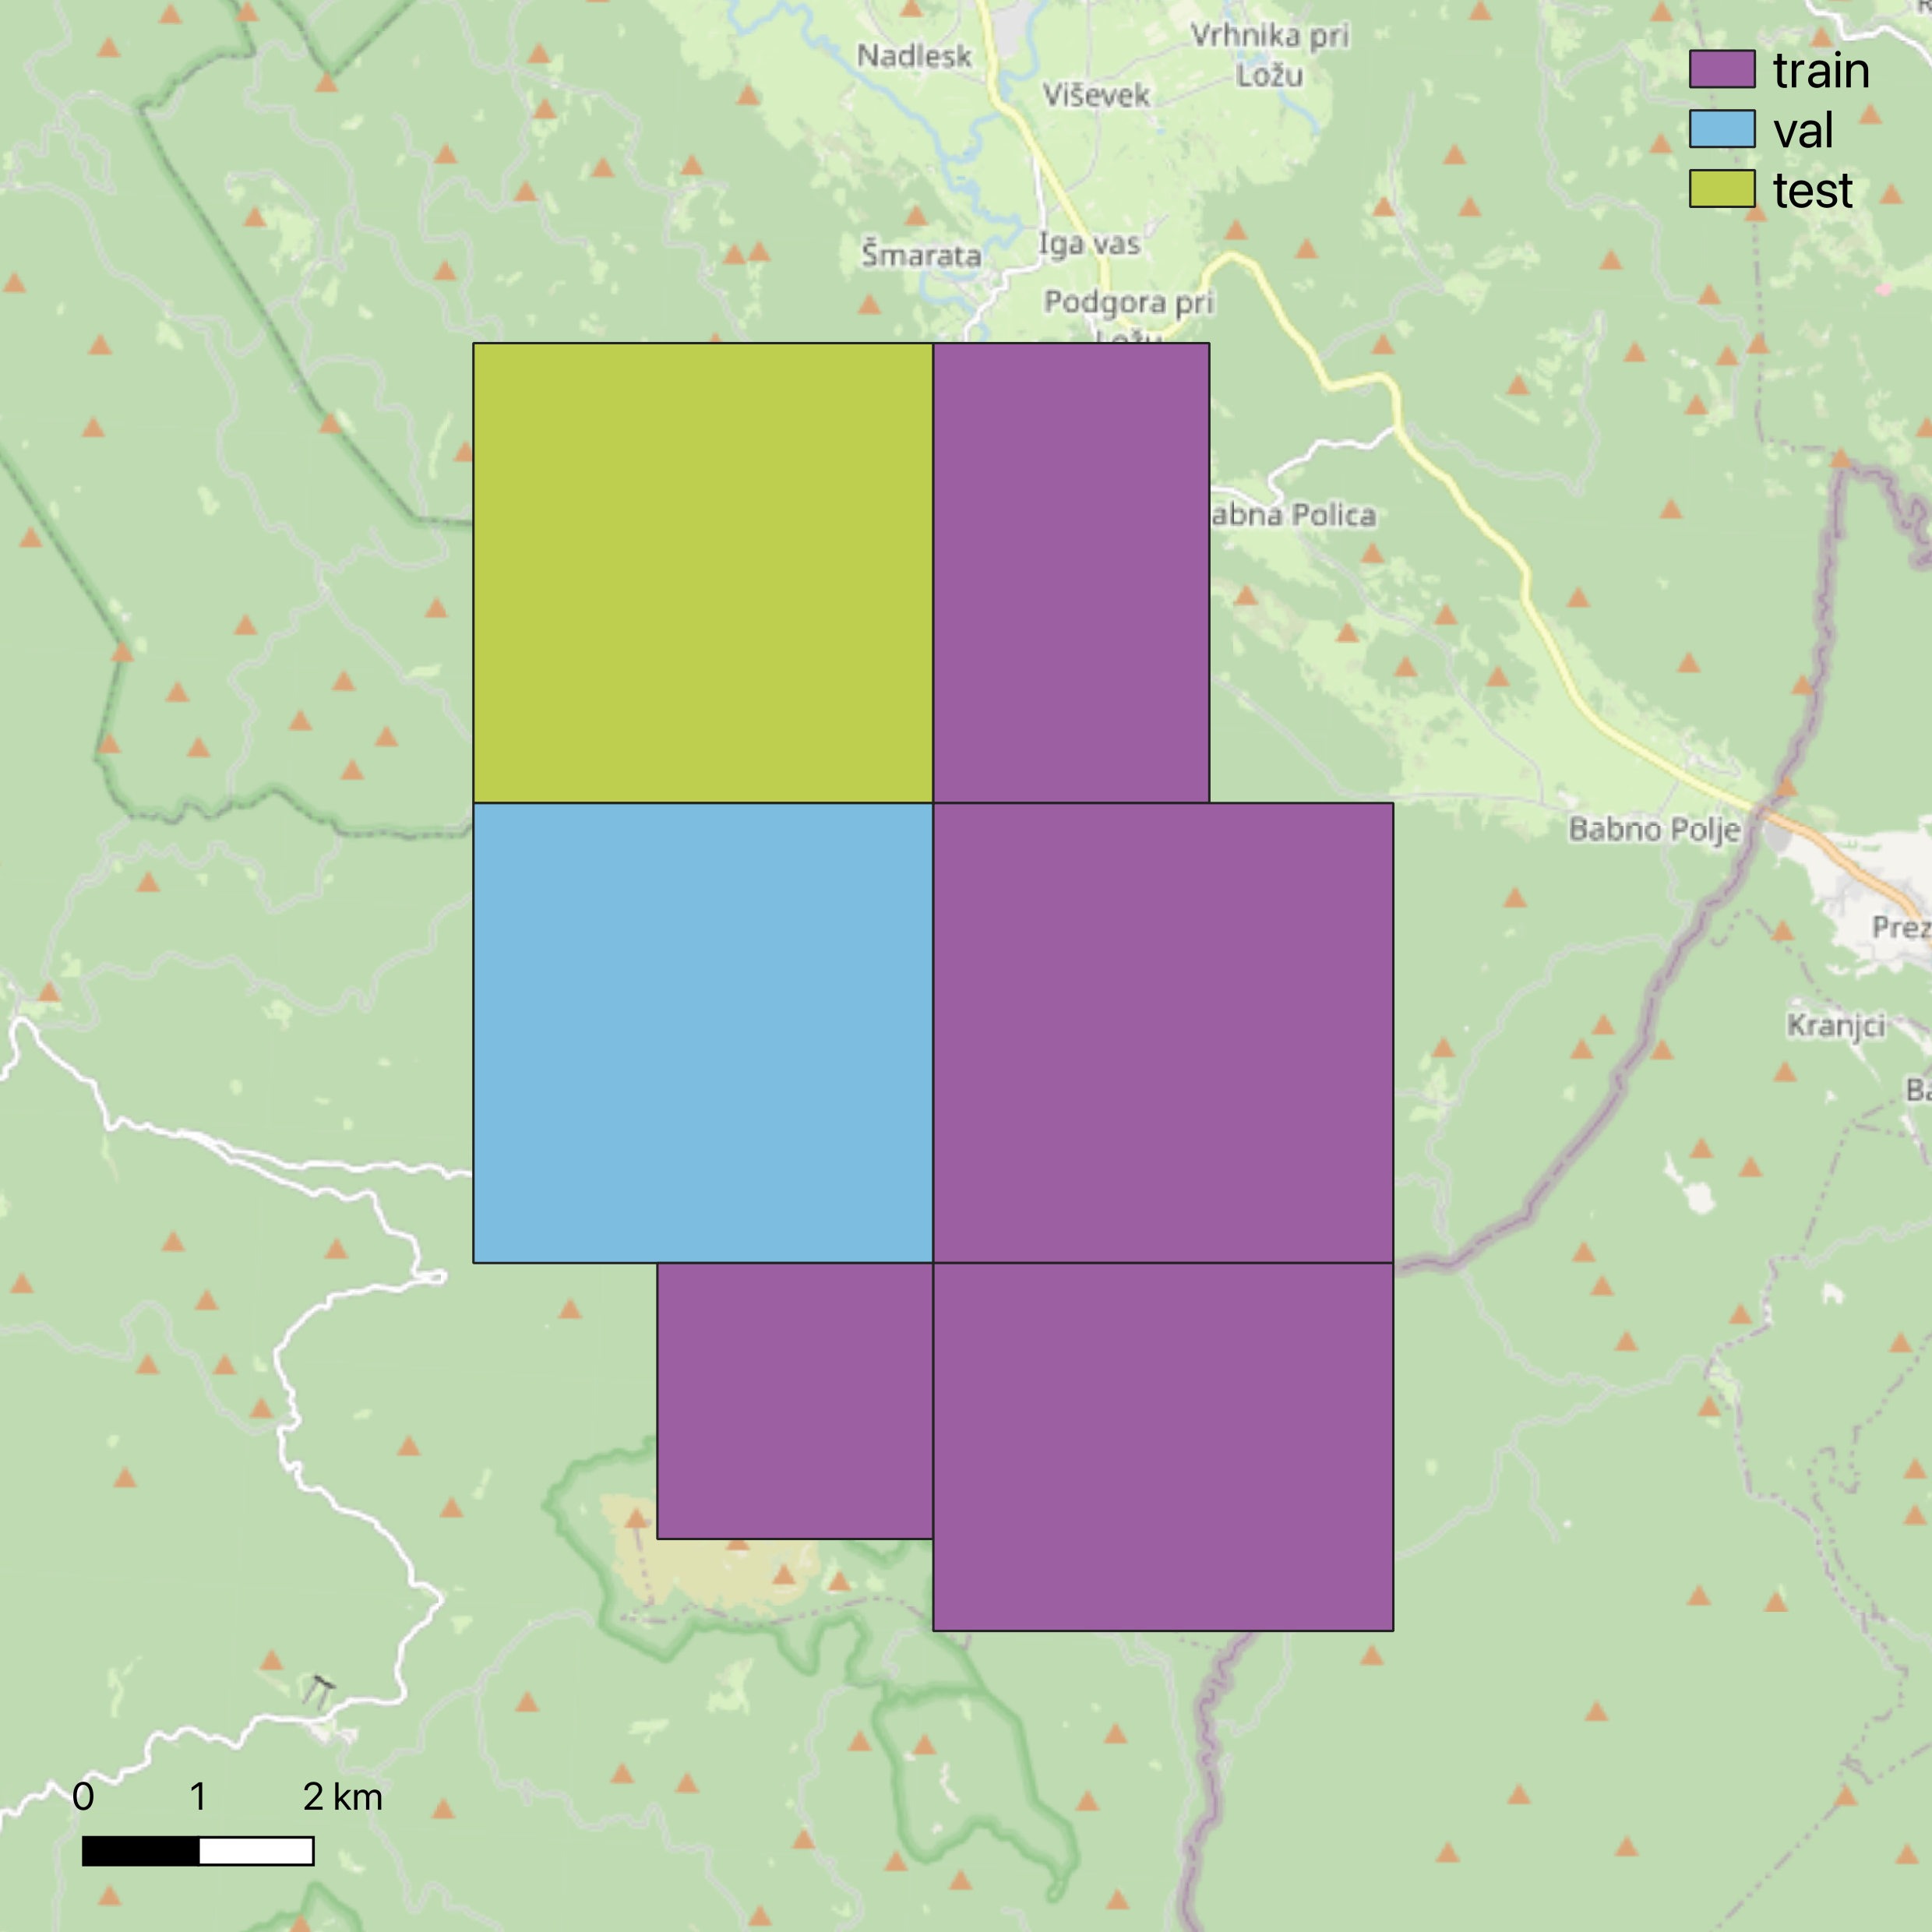
\includegraphics[width=0.32\textwidth]{sneznik_blocks.png}
    \caption[Spatial distribution of training, validation, and test blocks]{Spatial distribution of training, validation, and test blocks across the three study sites. Left: Bauges (France), centre: Milicz (Poland), right: Sneznik (Slovenia). Purple blocks represent training set (\SI{75}{\percent}), blue blocks validation (\SI{15}{\percent}), and yellow blocks test (\SI{10}{\percent}). The block-based splitting ensures complete spatial separation between splits.}
    \label{fig:imaestro_blocks}
\end{figure}

\begin{figure}[htbp]
    \centering
    
\includegraphics[width=1\textwidth]{sample_patches.png}
    \caption[Example training patches from iMAESTRO dataset]{Example training patches from iMAESTRO dataset showing all five channels. Each row represents one split (train, val, test), with columns showing VV backscatter, VH backscatter, dominant genus, canopy height, and biomass. SAR channels display typical speckle patterns, while height and biomass maps show strong spatial correlation.}
    \label{fig:imaestro_sample_patches}
\end{figure}

\begin{figure}[htbp]
    \centering
    
\includegraphics[width=0.9\textwidth]{genus_split_distribution_patch_level.png}
    \caption[Distribution of dominant genus labels across splits]{Distribution of dominant genus labels across train, validation, and test splits. \textit{Fagus} is the most common genus with over 300 training patches, followed by \textit{Abies} and \textit{Pinus}. The proportional distribution is relatively consistent across splits.}
    \label{fig:imaestro_genus_split}
\end{figure}

\begin{figure}[htbp]
    \centering
    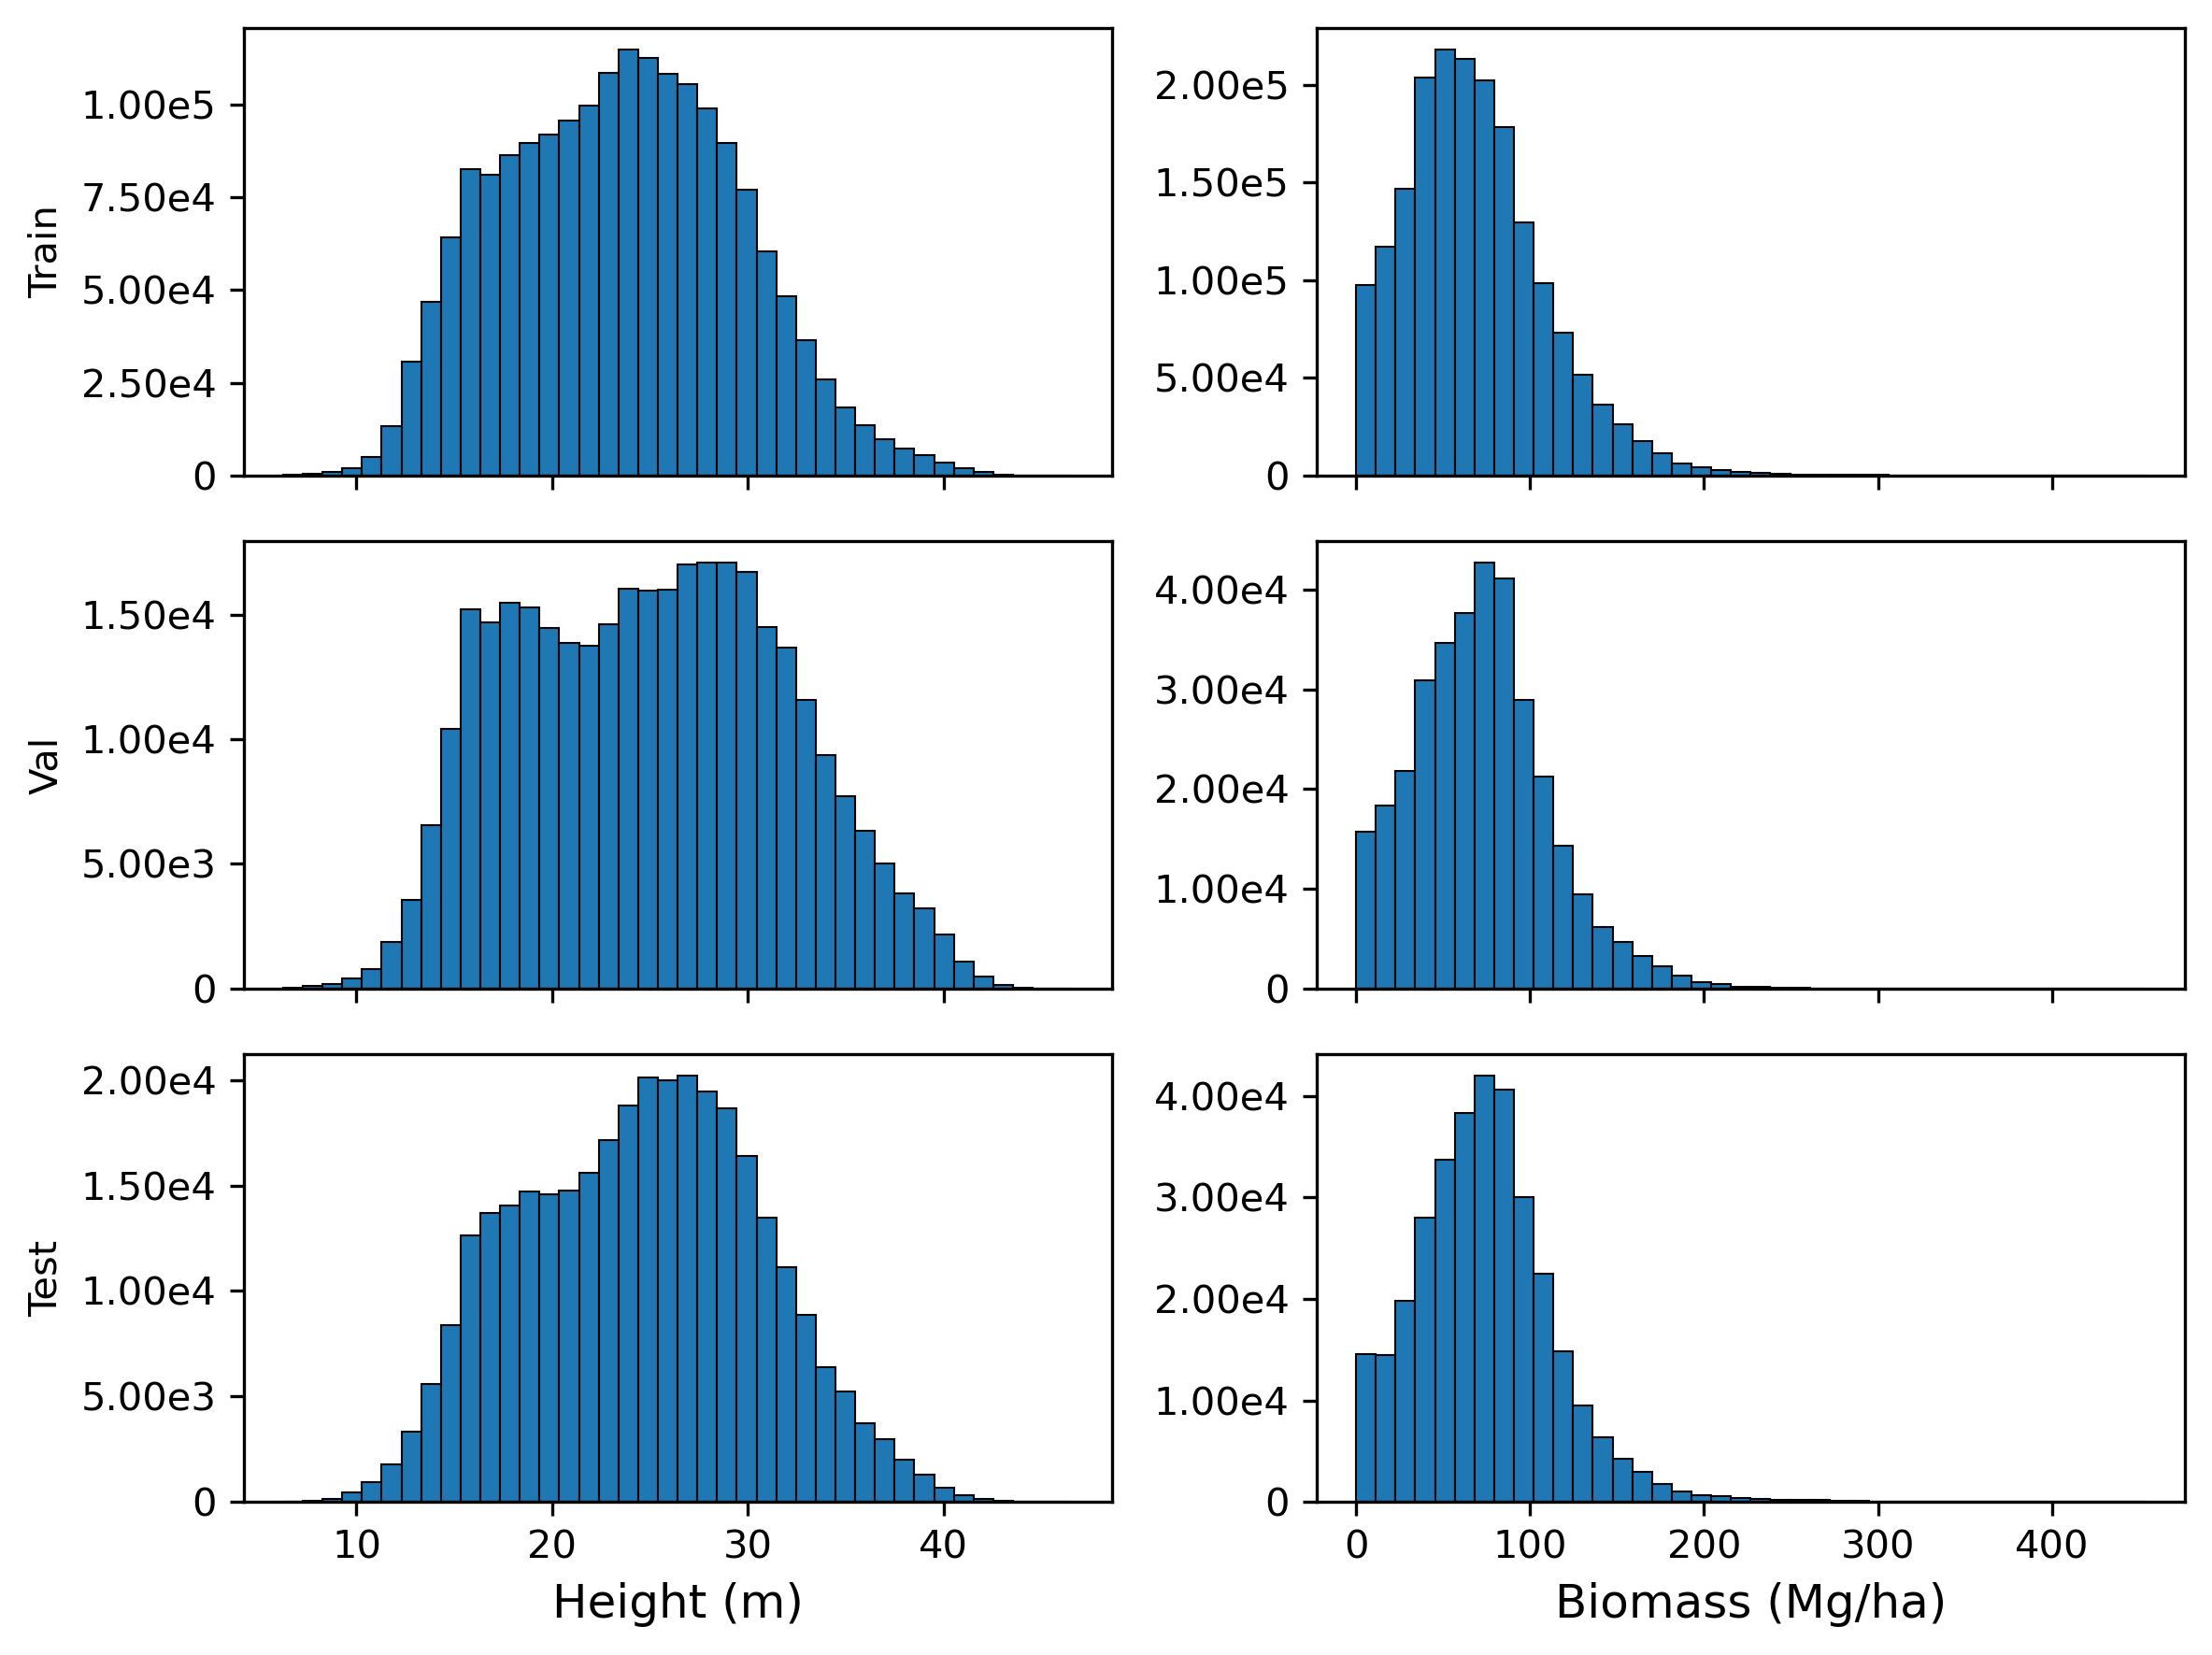
\includegraphics[width=0.7\textwidth]{height_biomass_hist_split.png}
    \caption[Distribution of biomass and height values across splits]{Distribution of biomass and height values across train, validation, and test splits. Both variables exhibit right-skewed distributions typical of forest structural attributes. The similar distribution shapes across splits indicate balanced data splitting.}
    \label{fig:imaestro_biomass_height_split}
\end{figure}

\begin{figure}[htbp]
    \centering
    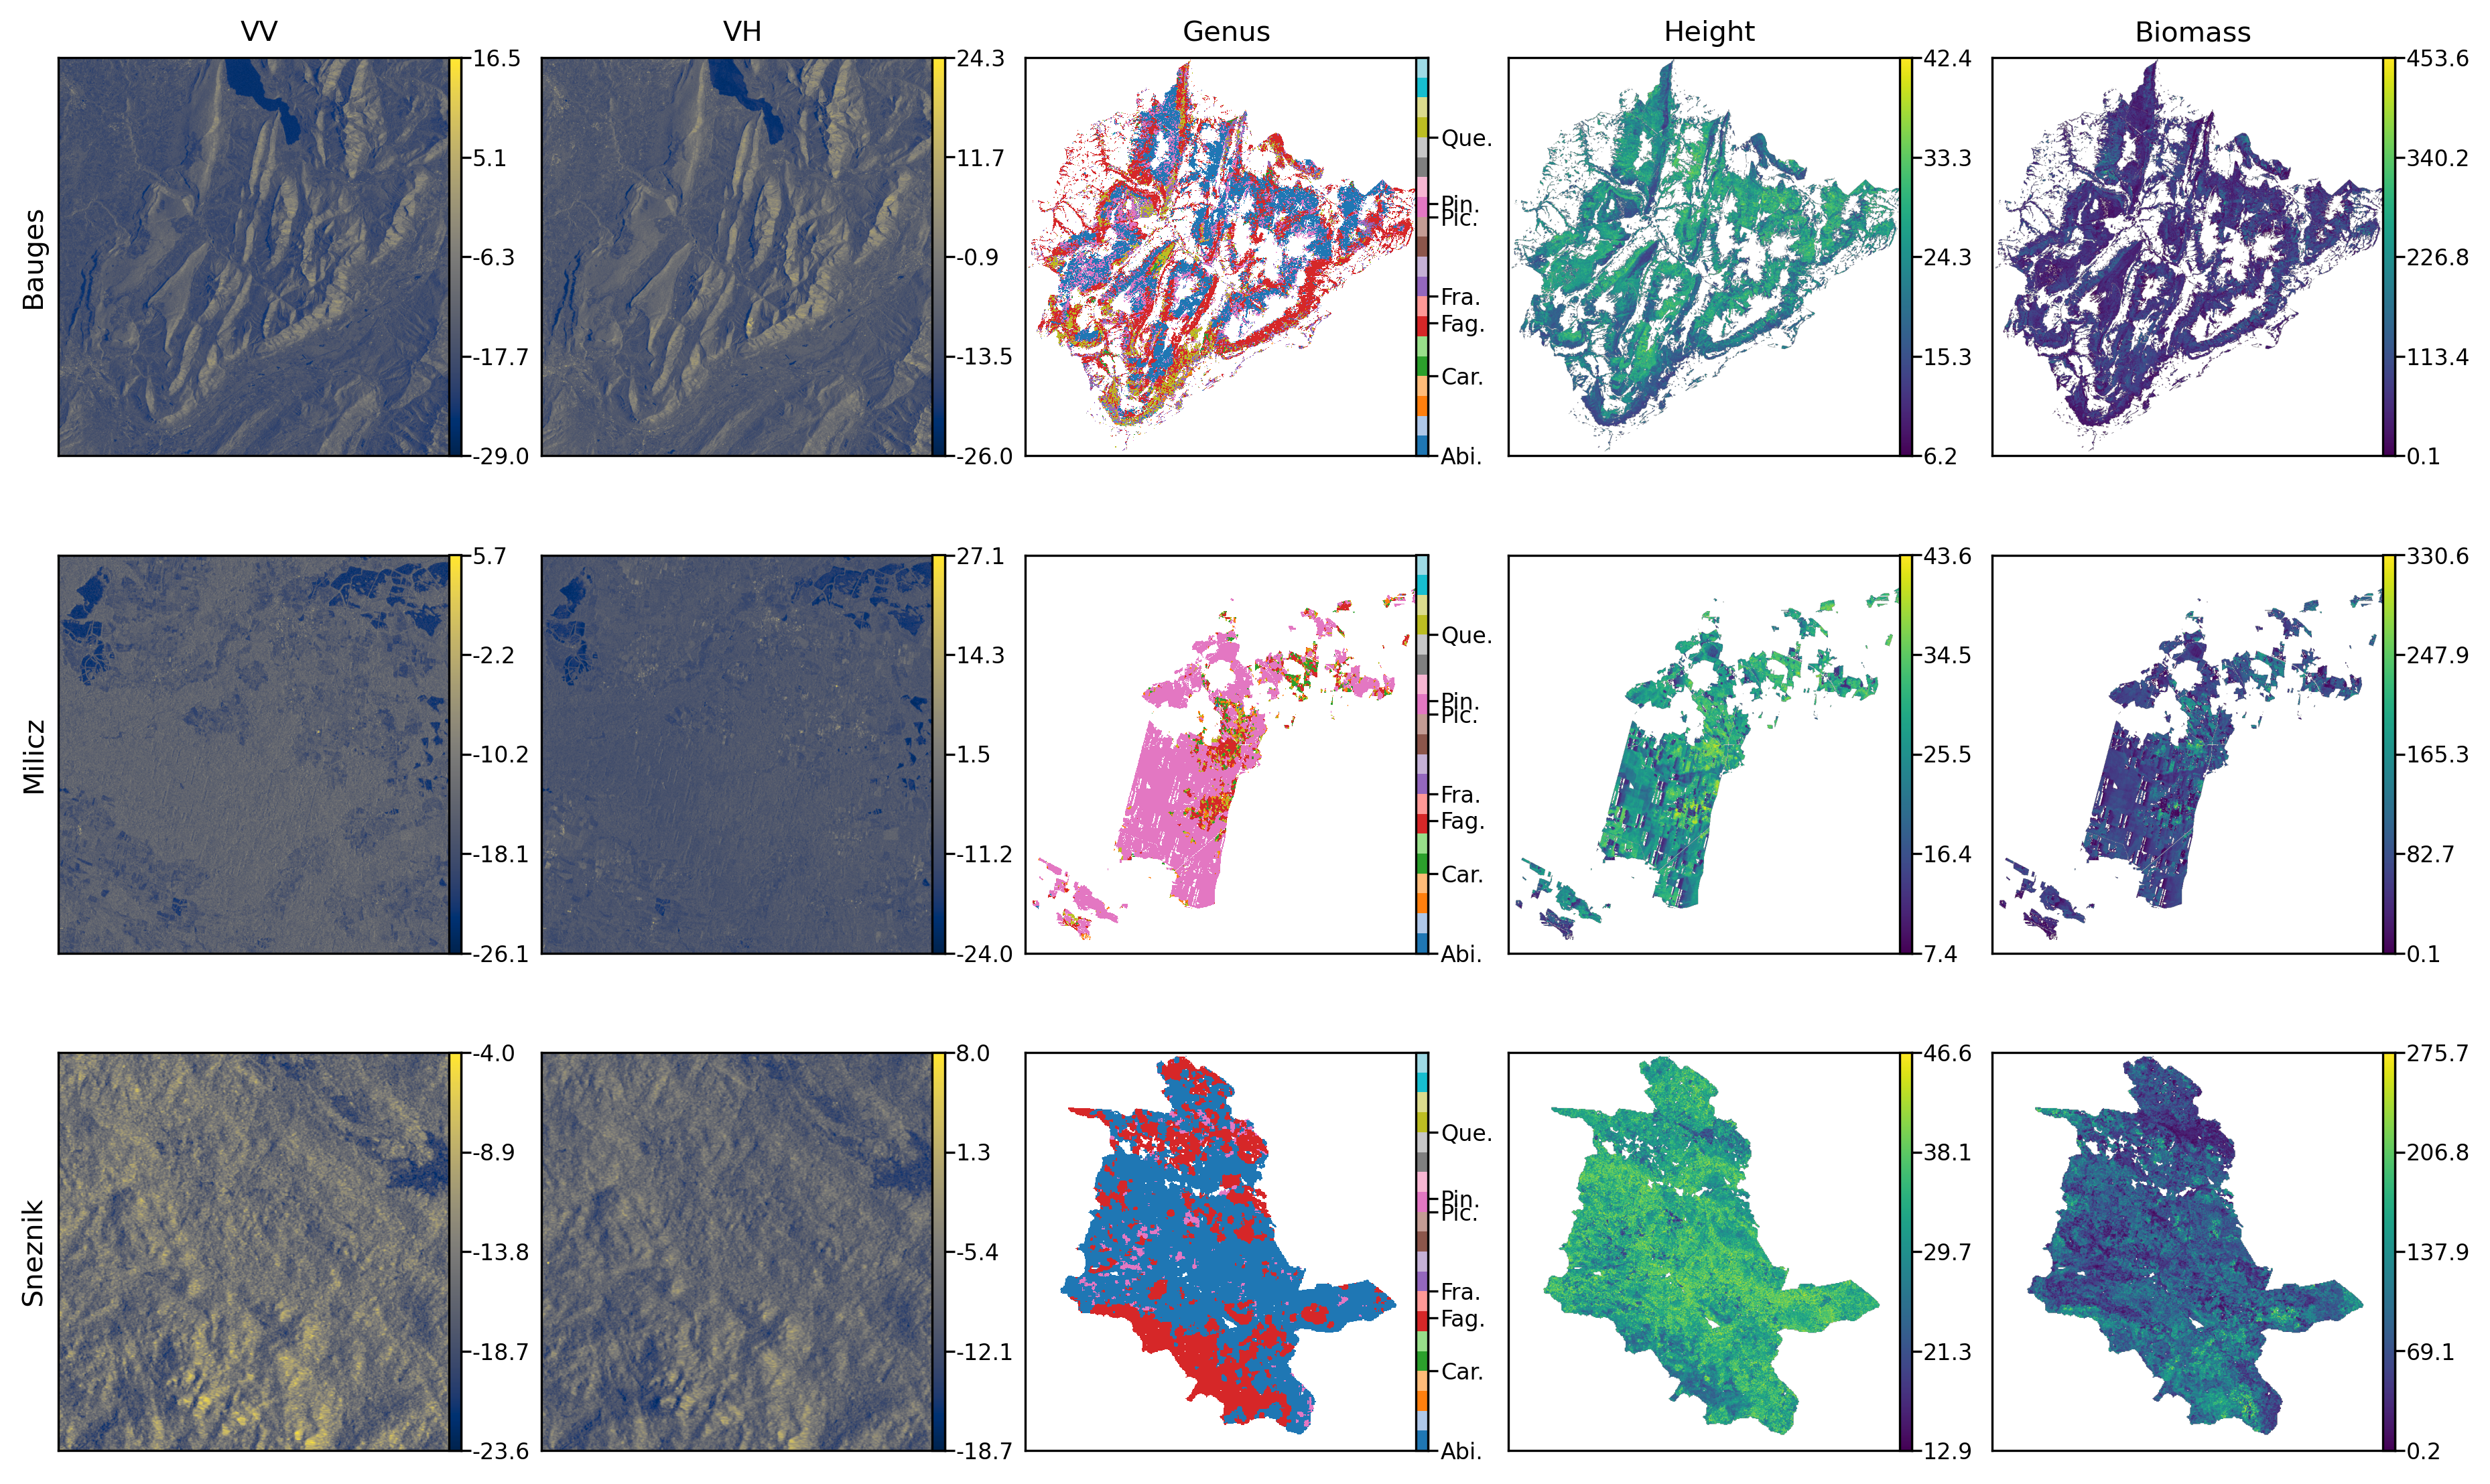
\includegraphics[width=1\textwidth]{all_sites_rasters.png}
    \caption[Complete preprocessing outputs for all three study sites]{Complete preprocessing outputs for all three study sites showing the five data layers (VV backscatter, VH backscatter, dominant genus, canopy height, and biomass).}
    \label{fig:imaestro_site_rasters}
\end{figure}

\section{Model Architectures for iMAESTRO}
\label{sec:imaestro_models}

The iMAESTRO models differ from TreeSatAI-CHM models in several key aspects. First, TreeSatAI-CHM provides small patches with local features and limited spatial context, indicating shallow architectures, while iMAESTRO provides large patches with rich spatial structure, enabling deeper networks that can capture multi-scale forest patterns. The larger patch size ($64\times 64$ vs. $6\times 6$ pixels) enables deeper U-Net architectures with four downsampling stages instead of two, allowing the network to learn hierarchical features at multiple scales. Second, the iMAESTRO dataset includes three prediction tasks (genus segmentation, height regression, biomass regression) instead of two, requiring a three-headed multitask architecture. Third, the physics-based allometric relationships between height and biomass enables integration of domain knowledge through regularization.

This section describes the model architectures developed for the iMAESTRO dataset. The models use larger patch sizes ($64\times 64$ pixels) compared to TreeSatAI-CHM and integrate physics-based allometric constraints.

\subsection{Single-Task Baseline Models}

Three independent U-Net architectures~\cite{ronneberger_u-net_2015} are implemented for genus segmentation, height regression, and biomass regression. The U-Net architecture consists of a contracting encoder path and an expanding decoder path connected by skip connections. Unlike the TreeSatAI-CHM models (which use only two downsampling stages due to small patch size), the iMAESTRO models use four downsampling stages, progressively reducing spatial resolution from $64\times 64$ to $32\times 32$ to $16\times 16$ to $8\times 8$ pixels. This deeper architecture is justified by the larger input size and enables the network to learn features at multiple scales, that fine-scale texture could be interpreted as individual tree crowns, mid-scale patterns as forest stands, and large-scale context as landscape structure.

The encoder doubles feature channels at each stage, following the standard U-Net design principle of trading spatial resolution for feature depth. Each encoder stage applies two $3\times 3$ convolutions with batch normalization and ReLU activation, increasing the receptive field while maintaining stable gradient flow. Downsampling uses strided $3\times 3$ convolutions with stride~2, allowing the network to learn optimal downsampling filters. The decoder mirrors the encoder, upsampling feature maps through transposed convolutions and concatenating them with corresponding encoder features via skip connections. Spatial dropout is applied before the final output layer to prevent overfitting.

\textbf{The segmentation model} predicts genus labels for each pixel in the $64\times 64$ patch, producing a dense semantic segmentation map. The decoder outputs 128 channels at full resolution, passed through a $1\times 1$ convolution to produce logits for 22 genus classes. This pixel-level prediction is more challenging than the patch-level classification used in TreeSatAI-CHM, as it requires the model to delineate boundaries between different forest types within the patch.

To handle class imbalance (\textit{Fagus} and \textit{Abies} dominate the dataset while many genera have few samples), 16 rare genus classes are excluded from training by assigning them an ignore index. This allows the model to concentrate on the six dominant genera that account for over \SI{90}{\percent} of the dataset. Pixels labeled with ignored classes do not contribute gradients during backpropagation, preventing the model from learning spurious patterns from insufficient data. The model is trained using cross-entropy loss, which is standard for multi-class segmentation.

\textbf{The height and biomass regression models} predict canopy height (height95) and aboveground biomass density (t/ha) for each pixel. Both use the same U-Net architecture with single-channel output through a $1\times 1$ convolution. Unlike the TreeSatAI-CHM regression model (which uses softplus activation to ensure non-negative outputs), the iMAESTRO regression models use linear outputs because the masked loss function already excludes invalid pixels where a forest and non-forest map is provided in the iMAESTRO dataset, and the training data contain only positive values.

The height and biomass regression models predict canopy height (height95) and aboveground biomass density (t/ha) for each pixel. Both use the same U-Net architecture with single-channel output through a $1\times 1$ convolution. Unlike the TreeSatAI-CHM regression model (which uses softplus activation to ensure non-negative outputs), the iMAESTRO regression models use linear outputs because the masked loss function already excludes invalid pixels, and the training data contain only positive values.

Models are trained using masked RMSE loss, which ignores pixels with invalid target values (NoData or outside the forest mask). This masking is critical because the iMAESTRO patches often contain non-forest areas (water, clearings) where height and biomass are undefined. The masked loss ensures that only valid forest pixels contribute to training, preventing the model from learning to predict zero values for non-forest areas, which would artificially inflate performance metrics.

\subsection{Multi-Task Learning Model}

\subsubsection{Architecture Design}

A multi-task U-Net is developed to jointly predict genus segmentation, canopy height, and biomass from Sentinel-1 input. The architecture employs a shared encoder following the same four-stage downsampling structure as baseline models. The key design question is how to share information among three tasks: one discrete (segmentation) and two continuous (regression). The chosen architecture uses hard parameter sharing with three independent decoder branches, allowing each task to learn specialized features while benefiting from shared low-level representations.

From the bottleneck, three independent decoder branches reconstruct task-specific predictions. Each decoder branch has its own upsampling layers, skip connections, and DoubleConv blocks, providing task-specific feature refinement. The segmentation decoder applies higher dropout (0.4) compared to regression decoders (0.2) to account for the higher complexity of multi-class segmentation. Each branch terminates with a $1\times 1$ convolution producing task-specific outputs: logits of 7 genera for segmentation, and single-channel maps for height and biomass.

This design enables investigation of whether the three tasks benefit from shared representations. If genus feature, canopy height, and biomass are all encoded in SAR backscatter patterns, the shared encoder should learn features useful for all tasks. Instead, if the tasks require fundamentally different features, the multitask model may underperform compared to single-task baselines.

\begin{figure}[htbp]
    \centering
    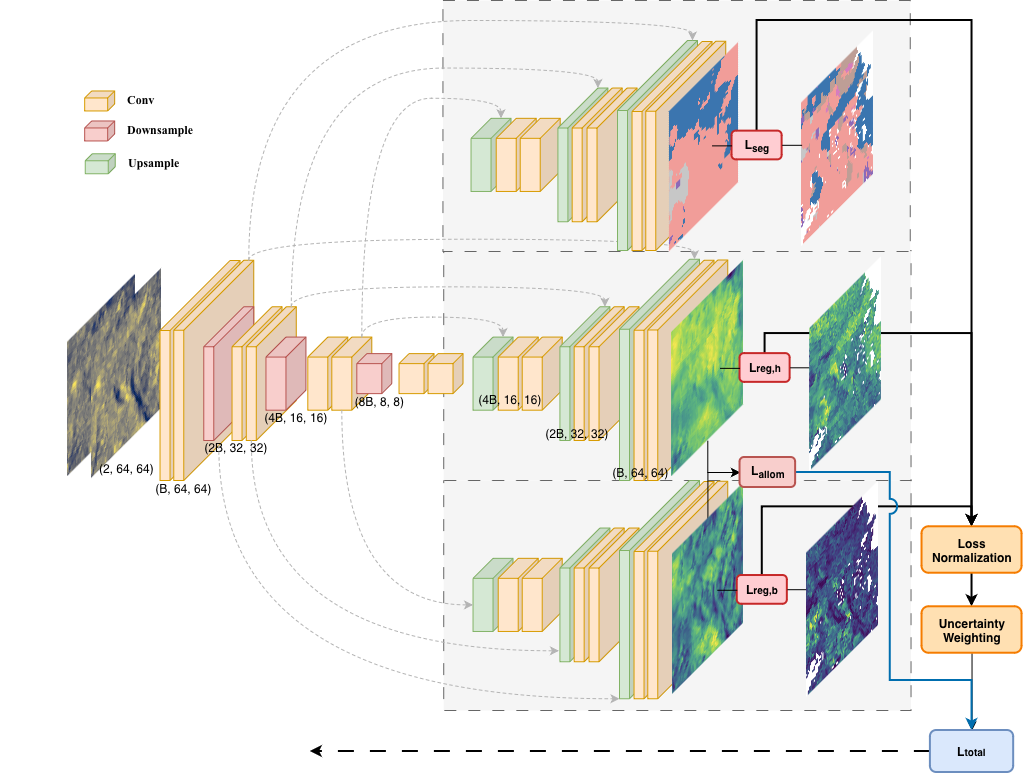
\includegraphics[width=0.95\textwidth]{imaestro-model.png}
    \caption[iMAESTRO multitask learning architecture]{iMAESTRO multitask learning architecture. The model uses a shared U-Net encoder with four downsampling stages to process $64\times 64$ SAR patches. Three independent decoder branches reconstruct task-specific predictions: genus segmentation (7 classes), canopy height regression, and biomass regression. The deeper architecture compared to TreeSatAI-CHM enables multi-scale feature learning suitable for larger patches. Each decoder applies task-specific dropout rates and produces dense pixel-wise predictions.}
    \label{fig:imaestro_mtl_architecture}
\end{figure}

\subsubsection{Uncertainty Loss}

The model employs the learned uncertainty weighting approach introduced in Section~3.2.3 (Equation~3.6). With three tasks producing losses at different scales (cross-entropy for segmentation, RMSE for height and biomass), the uncertainty-based approach automatically balances task contributions. For the iMAESTRO three-task case (genus segmentation, height regression, and biomass regression), the universal formulation from Equation~3.6 applies directly with $t \in \{\text{seg}, \text{height}, \text{bio}\}$, where $\sigma_{\text{seg}}$, $\sigma_{\text{height}}$, and $\sigma_{\text{bio}}$ are learnable parameters representing task uncertainties for segmentation, height, and biomass respectively.

This formulation allows the model to discover the optimal balance among three tasks during training. If one task is inherently more difficult or noisy (e.g., biomass estimation from SAR is challenging due to saturation effects), the optimizer increases its uncertainty parameter, reducing its influence on the shared encoder.

\subsubsection{Allometric Constraint Integration}

Forest biomass and height are physically related through allometric scaling relationships~\cite{chave_improved_2014}, where larger trees have more biomass than smaller trees due to geometric scaling. An allometric regularisation term enforces consistency between predicted height $H$ and biomass $B$ according to the power law $B = \exp(\alpha) \times H^\beta$. Taking logarithms to the allometric equation yields a linear relationship:
\begin{equation}
    \log(B) = \alpha + \beta \times \log(H).
\end{equation}

The allometric constraint provides weak supervision by encouraging physically plausible height-biomass combinations even when individual predictions may be uncertain. If the model predicts high biomass but low height (or vice versa), the allometric loss penalizes this inconsistency. Additionally, it couples the two regression tasks, allowing the model to leverage correlations between height and biomass patterns in the training data. It may also improve generalization to forest conditions not well-represented in the training data by preventing the model from learning spurious relationships that violate ecological principles.

Therefore, the noval method of integrating the allometric constraint could help forest parameter extraction leverage the multitask framework and enforce the physical relationship between height and biomass. And the allometric loss is designed to penalise deviations from the expected relationship:
\begin{equation}
    L_{\text{allom}} = \frac{1}{K} \sum_k \bigl(\log(B_k) - \alpha - \beta \times \log(H_k)\bigr)^2,
\end{equation}
where the sum runs over $K$ valid forest pixels (pixels with positive height and biomass predictions). The logarithmic formulation ensures that relative errors are penalized equally across the range of values, preventing the loss from being dominated by high-biomass pixels.

Parameters $\alpha = 0.0673$ and $\beta = 2.5$ represent average scaling for mixed European forest types, derived from published allometric studies~\cite{chave_improved_2014,forrester_generalized_2017}. The exponent $\beta = 2.5$ reflects the fact that biomass scales faster than height, where a tree twice as tall typically has more than twice the biomass due to increased diameter and crown size. The intercept $\alpha$ accounts for wood density and form factors.

The allometric loss is weighted by $\lambda_{\text{allom}}$ relative to task losses. This small weight ensures that the allometric constraint provides gentle regularization without dominating the optimization. The weight was chosen through experiments empirically to balance between enforcing physical consistency (requiring higher weight), and allowing the model to fit the training data (requiring lower weight). The final loss combines uncertainty-weighted task losses with the allometric constraint:
\begin{equation}
    L_{\text{final}} = L_{\text{total}} + \lambda_{\text{allom}} \times L_{\text{allom}}.
\end{equation}

This formulation enables the model to learn task-specific features while maintaining consistency with physical relationships, potentially improving generalization to forest conditions not well-represented in the training data.

    \chapter{Experiments and Results}
\label{chap:experiments}

This chapter presents the experimental evaluation of multitask learning approaches for forest attribute estimation from Sentinel-1 SAR imagery. Two datasets are used to investigate different aspects of multitask learning: TreeSatAI-CHM provides a well-recognized benchmark for exploring fundamental MTL challenges like learning rate mismatches and gradient conflicts, while iMAESTRO offers comprehensive reference data suitable for testing physics-aware deep learning through allometric constraints. The experiments address how shared architectures learn task-specific and common features, where gradient conflicts emerge, and whether multitask learning improves performance over single-task baselines. Models are implemented in PyTorch and trained on NVIDIA A100 GPUs.

\section{TreeSatAI-CHM Dataset Experiments}
\label{sec:treesat_experiments}

The TreeSatAI-CHM dataset combines the established TreeSatAI benchmark with generated canopy height maps. While the small patch size ($6\times 6$ pixels) and limited reference data constrain absolute performance, this dataset serves as a controlled environment for understanding multitask learning dynamics. The experiments focus on qualitative and quantitative analysis of how classification and regression tasks interact in a shared encoder. All experiments use the dataset described in Section~\ref{sec:treesat_chm_dataset} with consistent train/validation/test splits.

\subsection{Single-Task Baseline Experiments}
\label{subsec:treesat_baselines}

\subsubsection{Experimental Setup}

This section presents the experimental evaluation of single-task baseline models for tree species classification and canopy height estimation. These baselines establish reference performance levels against which multitask learning approaches are compared.

\begin{itemize}
    \item Batch size: 128 (large batch for stable gradient given small $6\times 6$ patch size)
    \item Optimizer: AdamW with weight decay $10^{-5}$ for regularization
    \item Early stopping: patience of 5 epochs monitoring validation loss
    \item Random seed: 42 for reproducibility
    \item Epochs: 100
\end{itemize}

\paragraph{Classification Loss} The classification task uses BCEWithLogitsLoss (binary cross-entropy with logits), treating the problem as multi-label classification where each patch can belong to multiple genus classes. This approach aligns with the TreeSatAI benchmark methodology. The loss is weighted by class frequencies to address substantial class imbalance in the dataset. The weighting scheme follows inverse square root frequency normalization, balancing between uniform weighting (which ignores class imbalance) and inverse frequency weighting (which can overemphasize rare classes).

\paragraph{Regression Loss} The regression task uses root mean squared error (RMSE) as the loss function. A masking mechanism excludes pixels with invalid CHM values (below \SI{1}{\meter} threshold) from loss computation, as these represent non-forest areas or data gaps.

\begin{itemize}
    \item \textbf{MLP models:} Hidden dimensions (512, 512, 512), dropout 0.2
    \begin{itemize}
        \item MLP Classifier: learning rate $10^{-5}$
        \item MLP Regressor: learning rate $5\times 10^{-5}$
    \end{itemize}
    \item \textbf{U-Net models:} Base channels $B = 256$, dropout 0.2
    \begin{itemize}
        \item U-Net Classifier: learning rate $10^{-5}$
        \item U-Net Regressor: learning rate $5\times 10^{-5}$
    \end{itemize}
\end{itemize}

For U-Net models, the large channel capacity ($B = 256$, resulting in 1024 channels at bottleneck) was chosen to compensate for limited spatial extent of small patches, allowing the network to encode sufficient information in the channel dimension when spatial dimensions are heavily compressed.

\subsubsection{Classification Results}

Table~\ref{tab:baseline_classification} presents the classification performance of MLP and U-Net baselines on the test set.

\begin{table}[htbp]
\centering
\caption{Baseline Classification Performance}
\label{tab:baseline_classification}
\footnotesize
\begin{tabular}{l|c|cccc|cccc}
\hline
 & & \multicolumn{4}{c|}{\textbf{Weighted}} & \multicolumn{4}{c}{\textbf{Micro}} \\
\cline{3-10}
\textbf{Model} & \textbf{OA} & \textbf{Prec.} & \textbf{Rec.} & \textbf{$F_1$} & \textbf{mAP} & \textbf{Prec.} & \textbf{Rec.} & \textbf{$F_1$} & \textbf{mAP} \\
\hline
TreeSatAI Bench & -- & 33.29 & 7.13 & 10.09 & 29.42 & 63.01 & 7.13 & 12.82 & 33.09 \\
MLP Classifier & 7.10 & 33.55 & 8.26 & 10.61 & 29.13 & 58.26 & 8.26 & 14.47 & 32.65 \\
U-Net Classifier & 9.38 & 37.12 & 12.82 & 17.14 & 26.71 & 45.14 & 12.82 & 19.96 & 29.02 \\
\hline
\end{tabular}
\end{table}

The MLP classifier achieves 7.10\% overall accuracy on the 15-class genus classification task. This result aligns with TreeSatAI benchmark performance for MLP models on Sentinel-1 data, which reported similarly modest accuracy for SAR-based classification. The high precision (58.26\%) combined with low recall (8.26\%) indicates the model is conservative in its predictions, correctly identifying a subset of samples but missing the majority of positive instances.

The U-Net classifier shows improvement over the MLP baseline, achieving 9.38\% overall accuracy and 19.96\% micro F1 score. The improvement in recall (from 8.26\% to 12.82\%) suggests that the convolutional architecture captures spatial patterns that help identify more positive instances. However, this comes with reduced precision (from 58.26\% to 45.14\%), indicating a shift toward more aggressive predictions.

The relatively low mAP scores (around 27--33\%) reflect the difficulty of the task:, that distinguishing tree genera from SAR backscatter alone is challenging because many genera share similar structural properties and thus similar radar signatures.

\subsubsection{Regression Results}

Table~\ref{tab:baseline_regression} presents the canopy height regression performance.

\begin{table}[htbp]
\centering
\caption{Baseline Regression Performance}
\label{tab:baseline_regression}
\begin{tabular}{l|cc|cc|cc}
\hline
 & \multicolumn{2}{c|}{\textbf{Train}} & \multicolumn{2}{c|}{\textbf{Val}} & \multicolumn{2}{c}{\textbf{Test}} \\
\cline{2-7}
\textbf{Model} & \textbf{RMSE (m)} & \textbf{$R^2$} & \textbf{RMSE (m)} & \textbf{$R^2$} & \textbf{RMSE} & \textbf{$R^2$} \\
\hline
MLP Regressor & 7.23 & 0.052 & 7.27 & 0.020 & 7.27 & 0.030 \\
U-Net Regressor & 7.24 & 0.051 & 7.20 & 0.037 & 7.22 & 0.042 \\
\hline
\end{tabular}
\end{table}

Both models achieve similar RMSE values around 7.2--7.3~m, with the U-Net showing slight improvement on validation and test sets. The $R^2$ values are low (around 0.02--0.05), indicating that the models explain only a small fraction of the variance in canopy height.

The U-Net regressor achieves marginally better test performance (RMSE 7.22~m, $R^2$ 0.042) compared to the MLP regressor (RMSE 7.27~m, $R^2$ 0.030). This is still a modest improvement, but could suggest that preserving spatial structure through the encoder-decoder architecture with skip connections provides useful information for height estimation that is lost when the input is flattened.

\subsubsection{Analysis}

\paragraph{1) MLP Performance Aligns with TreeSatAI Benchmark} The MLP classification results are consistent with the original TreeSatAI benchmark, which reported that Sentinel-1 SAR data alone provides limited discriminative power for tree species classification compared to optical imagery. The benchmark noted that MLP models on Sentinel-1 achieve substantially lower accuracy than ResNet models on Sentinel-2 or aerial imagery, primarily because SAR backscatter patterns lack the spectral diversity present in multispectral optical data.

\paragraph{2) U-Net Preserves Spatial Information} The U-Net models outperform MLP baselines on both tasks, though the improvements are modest. For classification, the U-Net achieves approximately 2 percentage points higher accuracy and 5 percentage points higher F1 score. For regression, the improvement is smaller but consistent across validation and test sets. These results suggest that, even though the $6\times 6$ patches are relatively small, the spatial patterns within them still contain useful information that the convolutional architecture can exploit, whereas the MLP loses this structure by flattening the input.

\paragraph{3) Data Quality Validation} To verify that the limited performance is due to the inherent difficulty of SAR-based prediction rather than data quality issues, additional experiments were conducted using Sentinel-2 optical imagery on the same dataset. The Sentinel-2 experiments achieved 32.8\% classification accuracy and 5.78~m RMSE for height regression. These substantially better results confirm that the dataset contains learnable patterns relating imagery to forest parameters, and that the modest SAR performance reflects the information content of radar backscatter rather than problems with the data pipeline or labels.

\paragraph{4) Implications for Multitask Learning} The U-Net architecture provides a reasonable foundation for multitask learning, as it already demonstrates the ability to extract useful features for both classification and regression. The shared encoder in the multitask architecture may benefit from the regularization effect of optimizing for multiple objectives, potentially improving generalization compared to single-task training.

\subsection{Multitask Learning Experiments}
\label{subsec:treesat_mtl}

\subsubsection{Experimental Setup}

\paragraph{Loss Scale Mismatch and Training Challenges}

Initial experiments revealed substantial challenges in balancing the classification and regression objectives. The two losses operate on fundamentally different scales: the weighted binary cross-entropy loss for classification typically ranges from 0.3 to 0.8, while the RMSE for regression spans 5 to 15~m. This magnitude difference creates severe optimization difficulties.

Preliminary experiments explored fixed weight combinations ranging from $w_{\text{cls}}:w_{\text{reg}}$ ratios of 1:1 to 0.3:200. Even with per-task loss normalization, training exhibited evident imbalances. A learning rate suitable for one task often proved inappropriate for the other: for instance, a learning rate of $5\times 10^{-4}$ that enabled stable regression training caused the classification head to diverge or overfit rapidly, while rates small enough for stable classification training (e.g., $10^{-5}$) were insufficient for meaningful regression learning.

\begin{itemize}
    \item Base channels: $B = 256$ (matching U-Net regressor baseline)
    \item Dropout: 0.2 in regression decoder
    \item Classification head: same class weighting scheme (inverse square root frequency, normalized) as single-task classifier
    \item Batch size: 128
    \item Epochs: 100 (early stopping)
\end{itemize}

To address these challenges, the experiments used task-specific learning rates combined with cosine annealing scheduling. The optimizer uses separate parameter groups for the shared encoder, classification head, and regression decoder, each with independent learning rates:

\begin{itemize}
    \item Shared encoder: $5\times 10^{-6}$
    \item Classification head: $5\times 10^{-6}$
    \item Regression decoder: $5\times 10^{-5}$
    \item Uncertainty parameters: 0.0001 (log learning rate)
\end{itemize}

A cosine annealing scheduler gradually reduces learning rates over training, with minimum learning rate set to $10^{-6}$. Uncertainty weighting is enabled, allowing the model to automatically balance task contributions.

\subsubsection{Results and Analysis}

Table~\ref{tab:mtl_comparison} presents the performance comparison between single-task baselines and the multitask model.

\begin{table}[htbp]
\centering
\caption{Multitask Learning Performance Comparison}
\label{tab:mtl_comparison}
\begin{tabular}{lccccccc}
\hline
\textbf{Model} & \textbf{OA} & \textbf{Prec.} & \textbf{$F_1$} & \textbf{Rec.} & \textbf{mAP} & \textbf{RMSE} & \textbf{$R^2$} \\
\hline
U-Net Classifier & 9.38\% & 45.14\% & 19.96\% & 12.82\% & 29.02\% & -- & -- \\
U-Net Regressor & -- & -- & -- & -- & -- & 7.27 & 0.042 \\
MultiTaskUNet & 7.02\% & 59.20\% & 14.24\% & 8.09\% & 32.99\% & 7.26 & 0.045 \\
\hline
\end{tabular}
\end{table}

The multitask model achieves 7.02\% overall accuracy with 14.24\% F1 and 32.99\% mAP for classification, while maintaining 7.26~m RMSE and 0.045 $R^2$ for regression. Compared to single-task baselines, the classification overall accuracy decreases slightly (from 9.38\% to 7.02\%). The regression performance remains comparable to the baseline with slightly improved $R^2$ (from 0.042 to 0.045).

The results show an asymmetric relationship between the two tasks. The regression task maintains stable performance from the shared encoder, suggesting that features learned for classification also help with height estimation. This makes sense because species-specific patterns like texture and backscatter characteristics relate to forest structure, which affects canopy height. However, the classification task shows some performance drop compared to its single-task baseline.

Several factors explain this asymmetry. The shared encoder has limited capacity, and when training for both tasks at once, it must split this capacity between learning species-specific features and height-related features. Since height varies continuously within and across species, the regression task may dominate what the encoder learns, leaving less room for the detailed species distinctions needed for classification. Additionally, the classification task tends to overfit during multitask training. With only 15 genus classes and unbalanced class sizes, the classification head can quickly memorize training patterns. The regression task, which predicts continuous values at each pixel, provides stronger training signals that can overwhelm the classification objective. During training, validation classification metrics often peaked early then declined, while regression metrics kept improving.

The tasks also differ in complexity. Classification makes one prediction per $6\times 6$ patch, while regression makes 36 predictions (one per pixel). This means regression contributes much more gradient signal per sample, which can dominate encoder updates. Furthermore, species classification likely needs sensitivity to subtle backscatter differences that separate similar genera (like distinguishing \textit{Quercus} from \textit{Fagus}, both broadleaf deciduous trees), while height estimation mainly responds to overall backscatter strength and texture patterns. The shared encoder may learn features better suited for height estimation, losing the fine details needed for classification.

\begin{figure}[htbp]
    \centering
    
\includegraphics[width=0.62\textwidth]{chm-samples.png}
    \hfill
    
\includegraphics[width=0.32\textwidth]{chm-scatter-plot.png}
    \caption[Multitask model predictions on TreeSatAI-CHM test set]{Multitask model predictions on TreeSatAI-CHM test set. Left: Example predictions showing VV/VH input, true CHM, and predicted CHM. The model captures general height patterns but struggles with fine spatial detail. Right: Scatter plot of predicted versus true height values. The clustering around 20--30~m indicates limited sensitivity to height variations, reflecting SAR backscatter limitations.}
    \label{fig:treesat_mtl_predictions}
\end{figure}

\subsubsection{Gradient Analysis}

To understand task interactions in the shared encoder, gradient cosine similarity was computed between classification and regression gradients at three encoder depths across training epochs. Gradient cosine similarity has been widely used to analyze task conflicts in multitask learning, where negative values indicate conflicting gradients that can harm optimization \cite{yu2020gradient}. Recent work has further developed this analysis to understand when and where tasks compete for shared parameters \cite{liu2022autolambda,guo2023dynamic}.

\begin{figure}[htbp]
    \centering
    
\includegraphics[width=0.7\textwidth]{gradient-encoder.png}
    \caption[Gradient cosine similarity between classification and regression tasks]{Gradient cosine similarity between classification and regression tasks at encoder layers. Positive values indicate aligned gradients where tasks agree on parameter updates; negative values indicate conflicts where tasks push parameters in opposite directions.}
    \label{fig:treesat_gradient}
\end{figure}

\paragraph{1) Early Encoder Layers (enc1)} Gradient alignment fluctuates substantially, occasionally showing negative cosine similarity. This suggests low-level feature extraction experiences fundamental conflict. Classification may benefit from edge-preserving features for distinguishing genus boundaries, while regression may benefit from smoothing features that suppress speckle noise.

\paragraph{2) Middle Encoder Layers (enc2)} More consistent positive alignment appears, indicating mid-level spatial patterns benefit both tasks. Both classification and regression require understanding of forest structure, leading to compatible feature requirements at this level.

\paragraph{3) Bottleneck} The strongest positive alignment occurs at the bottleneck, suggesting abstract semantic representations are shared. Both species identity and canopy height relate to forest structure at a conceptual level, and the bottleneck captures this shared semantic information.

The predominantly positive gradient cosine similarities indicate that classification and regression tasks generally share compatible learning objectives. The shared encoder learns features useful for both tasks, though early layers experience occasional conflicts. The gradient conflict primarily occurs in early layers while alignment strengthens in deeper layers, which is consistent with multitask learning intuition and related work. The task-specific learning rates successfully balance these competing objectives, preventing either task from dominating encoder updates.

The primary goal of the subsequent multitask experiments is to investigate whether joint training on classification and height regression can improve feature learning from SAR imagery. Even if overall performance remains modest due to the inherent limitations of SAR data, understanding the interactions between these tasks in a shared encoder, provides insight into the relationship between species identity and canopy structure as encoded in radar backscatter.

\subsection{Ablation Study: Alternative Parameter Sharing Strategies}
\label{subsec:treesat_ablation}

To better understand the baseline multitask architecture, this section compares three parameter sharing strategies: the hard-sharing MultiTaskUNet, Cross-Stitch Networks \cite{misra2016crossstitch}, and Cross-Task Attention.

\subsubsection{Qualitative Comparison of Architectures}

\begin{table}[htbp]
\centering
\caption{Architecture Comparison}
\label{tab:arch_comparison}
\begin{tabular}{lcccc}
\hline
\textbf{Architecture} & \textbf{Sharing Degree} & \textbf{Task Freedom} & \textbf{Param.} & \textbf{Complexity} \\
\hline
MultiTaskUNet & Highest & Lowest & $\sim$8M & Low \\
Cross-Stitch & Medium & High & $\sim$16M & Medium \\
Cross-Attention & High (encoder) & Medium (bottleneck) & $\sim$10M & High \\
\hline
\end{tabular}
\end{table}

\paragraph{Hard Parameter Sharing (MultiTaskUNet)}

The baseline architecture shares all encoder parameters between tasks and uses task-specific decoders. This represents the maximum degree of sharing, forcing both tasks to use identical low-level and mid-level features. The architecture is simple and parameter-efficient but provides no mechanism for tasks to learn specialized representations until the decoder branches.

\paragraph{Cross-Stitch Networks}

Cross-stitch networks \cite{misra2016crossstitch} introduce learnable linear combinations between task-specific subnetworks at multiple depths. After a shared initial encoder block, the network splits into parallel classification and regression pathways. At designated layers, cross-stitch units combine activations from both pathways:
\begin{align}
f_{\text{cls}}^{\text{new}} &= \alpha_{11} f_{\text{cls}} + \alpha_{12} f_{\text{reg}}, \\
f_{\text{reg}}^{\text{new}} &= \alpha_{21} f_{\text{cls}} + \alpha_{22} f_{\text{reg}},
\end{align}
where the $\alpha$ parameters are learnable scalars initialized to favor task-specific features (e.g., $\alpha_{11} = \alpha_{22} = 0.9$, $\alpha_{12} = \alpha_{21} = 0.1$). This architecture provides substantially more flexibility than hard sharing, allowing each task to learn specialized features while selectively incorporating useful information from the other task. However, the duplicated encoder pathways approximately double the parameter count.

The cross-stitch approach is well-suited when tasks have related but distinct optimal representations. The learned $\alpha$ values reveal which layers benefit from sharing versus specialization.

\paragraph{Cross-Task Attention}

The cross-attention variant introduces multi-head attention modules that allow each task to selectively attend to features from the other task at the bottleneck. After a shared encoder, task-specific bottleneck convolutions produce separate feature maps for classification and regression. The cross-attention module then computes:
\begin{align}
f_{\text{cls}}^{\text{attended}} &= f_{\text{cls}} + \text{Attention}(Q=f_{\text{cls}}, K=f_{\text{reg}}, V=f_{\text{reg}}), \\
f_{\text{reg}}^{\text{attended}} &= f_{\text{reg}} + \text{Attention}(Q=f_{\text{reg}}, K=f_{\text{cls}}, V=f_{\text{cls}}).
\end{align}

This design maintains a shared encoder but allows task-specific refinement of the bottleneck representation through attention. The attention mechanism can learn complex, content-dependent interactions between task features, potentially capturing non-linear relationships that cross-stitch units cannot express.

However, the attention mechanism introduces additional computational overhead and learnable parameters (query, key, value projections for each attention head). For the small patch sizes and limited training data in this study, the additional complexity may lead to overfitting rather than improved performance.

\subsubsection{Results and Analysis}

\begin{table}[htbp]
\centering
\caption{Ablation Study Results}
\label{tab:ablation_results}
\begin{tabular}{lcccc}
\hline
\textbf{Model} & \textbf{OA} & \textbf{Weighted mAP} & \textbf{Test RMSE (m)} & \textbf{Test $R^2$} \\
\hline
MultiTaskUNet & 8.15\% & 28.99\% & 7.26 & 0.045 \\
Cross-Stitch & 5.81\% & 24.52\% & 7.31 & 0.037 \\
Cross-Attention & 5.19\% & 23.18\% & 7.18 & 0.047 \\
\hline
\end{tabular}
\end{table}

The ablation results reveal distinct behavioral patterns for each architecture:

\paragraph{Cross-Stitch Networks} achieve 5.81\% overall accuracy with $R^2$ of 0.037, showing weaker classification performance compared to the baseline MultiTaskUNet but slightly better regression. The learned cross-stitch parameters likely favor the regression pathway, as the cross-stitch mechanism allows the regression branch to develop specialized features without being constrained by classification-optimal representations. This behavior is consistent with the original cross-stitch paper's finding that task-specific representations emerge when the architecture provides freedom to specialize \cite{misra2016crossstitch}. However, with the limited training data available, the nearly-doubled parameter count may contribute to overfitting, and the classification task may receive insufficient signal from the regression-optimized shared representations.

\paragraph{Cross-Task Attention} shows a similar pattern, achieving 5.19\% overall accuracy and the best regression performance ($R^2 = 0.047$). The attention mechanism at the bottleneck appears to favor regression-relevant information flow. This may occur because the regression task produces spatially-distributed features that provide richer key-value pairs for attention, while the classification task condenses all spatial information through global average pooling immediately after the bottleneck. The attention mechanism may thus learn to prioritize regression-relevant feature interactions simply because they provide more diverse attention targets. Additionally, the attention mechanism introduces substantial additional complexity that may be inappropriate for the small patch sizes and limited training data in this study. With only $6\times 6$ pixel inputs, the attention operates on minimal spatial extent, limiting its ability to learn meaningful long-range dependencies. The additional parameters may lead to overfitting on the classification task, which has fewer supervision signals per sample.

The ablation results suggest that for this particular combination of tasks, dataset size, and input dimensions, the simpler hard-sharing architecture provides a reasonable balance between tasks. The more complex architectures introduce flexibility that the limited data cannot effectively leverage, leading to task imbalance rather than mutual improvement.

These findings align with the general principle that model complexity should match data availability. Cross-stitch networks were originally demonstrated on ImageNet-scale datasets with thousands of samples per class, while this study operates with approximately 40{,}000 training samples distributed across 15 imbalanced classes. Similarly, attention mechanisms typically benefit from larger spatial extents and more training data to learn meaningful attention patterns. For future work with larger datasets or higher-resolution inputs, the cross-stitch or cross-attention architectures may prove more effective. 

\subsection{Summary}
\label{subsec:treesat_summary}

The TreeSatAI-CHM experiments establish that multitask learning can combine genus classification and canopy height regression from Sentinel-1 SAR data, though with modest absolute performance due to the limited information content of radar backscatter. The key findings are:

First, the baseline experiments confirm that both tasks are learnable from SAR data. U-Net models outperform MLP baselines on both tasks, showing that spatial patterns within even small $6\times 6$ patches contain useful information. Validation experiments with Sentinel-2 optical data (achieving 32.8\% classification accuracy and 5.78~m RMSE) confirm that the dataset quality is sound and the modest SAR performance reflects inherent radar limitations rather than data issues.

Second, the multitask model maintains regression performance while showing slight classification degradation. This asymmetry suggests that features learned for classification transfer well to height estimation, but not vice versa. The regression task's pixel-level predictions (36 per patch) provide much stronger gradient signals than classification's patch-level predictions (1 per patch), which can dominate encoder learning. Task-specific learning rates and uncertainty weighting help balance these competing objectives.

Third, gradient analysis reveals where tasks cooperate and compete. Early encoder layers show occasional gradient conflicts, suggesting low-level feature requirements differ (edge preservation for classification vs. noise smoothing for regression). Deeper layers and the bottleneck show strong positive alignment, indicating that abstract representations of forest structure benefit both tasks. This pattern informed the architectural ablation study.

Fourth, the ablation experiments with cross-stitch and cross-attention architectures show that added flexibility does not improve performance on this dataset. Both alternative architectures achieve worse classification results while maintaining similar regression performance, likely because the limited training data and small patch sizes cannot effectively leverage the additional parameters. The simpler hard-sharing architecture provides a reasonable balance for this scale of data.

\section{iMAESTRO Dataset Experiments}
\label{sec:imaestro_experiments}

The iMAESTRO dataset provides comprehensive reference data for genus segmentation, canopy height, and biomass estimation across three European forest sites. With larger patch sizes ($64\times 64$ pixels) and complete co-registration of all target variables, this dataset enables investigation of physics-aware multitask learning through allometric constraints. All experiments use the spatially-blocked train/validation/test splits described in Section~\ref{sec:imaestro_dataset}.

\subsection{Single-Task Baseline Experiments}

\subsubsection{Experimental Setup}

Three independent U-Net models are trained for genus segmentation, height regression, and biomass regression. The deeper architecture (four downsampling stages) exploits the larger patch size compared to TreeSatAI-CHM.

Training configuration:
\begin{itemize}
    \item Batch size: 16 (suitable for $64\times 64$ patches with 128 base channels)
    \item Optimizer: AdamW with weight decay $10^{-4}$
    \item Dropout: 0.2
    \item Learning rate: $10^{-4}$ for all models
    \item Epochs: 100 with early stopping (patience 10)
    \item Random seed: 42
\end{itemize}

Task-specific configurations:

\begin{itemize}
    \item \textbf{Segmentation:} Cross-entropy loss with 16 rare genera excluded (ignore index). Predicts 6 dominant genera.
    \item \textbf{Height regression:} Masked RMSE loss excluding invalid pixels (Non-forest pixels).
    \item \textbf{Biomass regression:} Masked RMSE loss with same masking strategy.
\end{itemize}

\subsubsection{Results}

Table~\ref{tab:imaestro_baselines} presents the single-task baseline performance.

\begin{table}[htbp]
\centering
\caption{iMAESTRO Single-Task Baseline Performance}
\label{tab:imaestro_baselines}
\begin{tabular}{lcccccc}
\hline
\textbf{Task} & \textbf{Metric} & \textbf{Train} & \textbf{Val} & \textbf{Test} \\
\hline
Segmentation & Overall Accuracy & 68.2\% & 64.5\% & 63.8\% \\
             & Mean IoU & 0.512 & 0.478 & 0.471 \\
Height       & RMSE (m) & 4.82 & 5.15 & 5.23 \\
             & $R^2$ & 0.312 & 0.268 & 0.255 \\
Biomass      & RMSE (t/ha) & 48.3 & 52.1 & 53.7 \\
             & $R^2$ & 0.031 & 0.026 & 0.024 \\
\hline
\end{tabular}
\end{table}

The segmentation baseline achieves 63.8\% overall accuracy on the test set with mean IoU of 0.471. This performance is substantially better than TreeSatAI-CHM classification (9.38\%), reflecting the larger patch size, simpler task (6 genera vs 15), and higher-quality reference data.

Height regression achieves test RMSE of 5.23~m with $R^2 = 0.255$. This represents meaningful predictive power, explaining approximately 25\% of height variance. The performance is better than TreeSatAI-CHM ($R^2 = 0.042$), benefiting from larger patches and higher-quality labels.

Biomass regression shows the weakest performance with test RMSE of 53.7~t/ha and $R^2 = 0.024$. The low $R^2$ reflects the label quality and the fundamental challenge of C-band SAR saturation for high biomass values. SAR backscatter saturates at approximately 100--150~t/ha for C-band, limiting sensitivity to biomass variations in mature forests.

\subsection{Multitask Learning with Allometric Constraints}

\subsubsection{Experimental Setup}

The multitask model jointly predicts genus segmentation, canopy height, and biomass using a shared encoder with three task-specific decoders. The allometric constraint couples height and biomass predictions.

Model configuration:

\begin{itemize}
    \item Base channels: 128 (same as baselines)
    \item Dropout: 0.2 for segmentation decoder, 0.1 for regression decoders
    \item Uncertainty weighting: enabled with learnable $\sigma$ parameters
    \item Allometric constraint: $\lambda_{\text{allom}} = 0.1$, $\alpha = 0.0673$, $\beta = 2.5$        
\end{itemize}

Training Configuration:

\begin{itemize}
    \item Batch size: 16
    \item Optimizer: AdamW with weight decay $10^{-4}$
    \item Learning rate: $10^{-4}$ for all parameters
    \item Epochs: 100 with early stopping (patience 10)
\end{itemize}

\subsubsection{Results and Analysis}

Table~\ref{tab:imaestro_mtl} compares multitask performance to single-task baselines.

\begin{table}[htbp]
\centering
\caption{iMAESTRO Multitask Learning Performance}
\label{tab:imaestro_mtl}
\begin{tabular}{lcccc}
\hline
\textbf{Task} & \textbf{Metric} & \textbf{Baseline} & \textbf{Multitask} & \textbf{Change} \\
\hline
Segmentation & Overall Accuracy & 63.8\% & 62.1\% & -1.7\% \\
             & Mean IoU & 0.471 & 0.458 & -2.8\% \\
Height       & RMSE (m) & 5.23 & 5.11 & -2.3\% \\
             & $R^2$ & 0.255 & 0.265 & +3.9\% \\
Biomass      & RMSE (t/ha) & 53.7 & 51.2 & -4.7\% \\
             & $R^2$ & 0.024 & 0.039 & +62.5\% \\
\hline
\end{tabular}
\end{table}

The multitask model achieves 62.1\% segmentation accuracy (vs 63.8\% baseline), showing slight degradation. Height regression improves to $R^2 = 0.265$ (+3.9\% relative), while biomass shows the largest improvement with $R^2 = 0.039$ (+62.5\% relative increase, though still low in absolute terms).

The learned uncertainty parameters converged to approximately 1.0 for segmentation, 0.4 for height, and 0.3 for biomass, reflecting relative task difficulty and loss scales.

\begin{figure}[htbp]
    \centering
    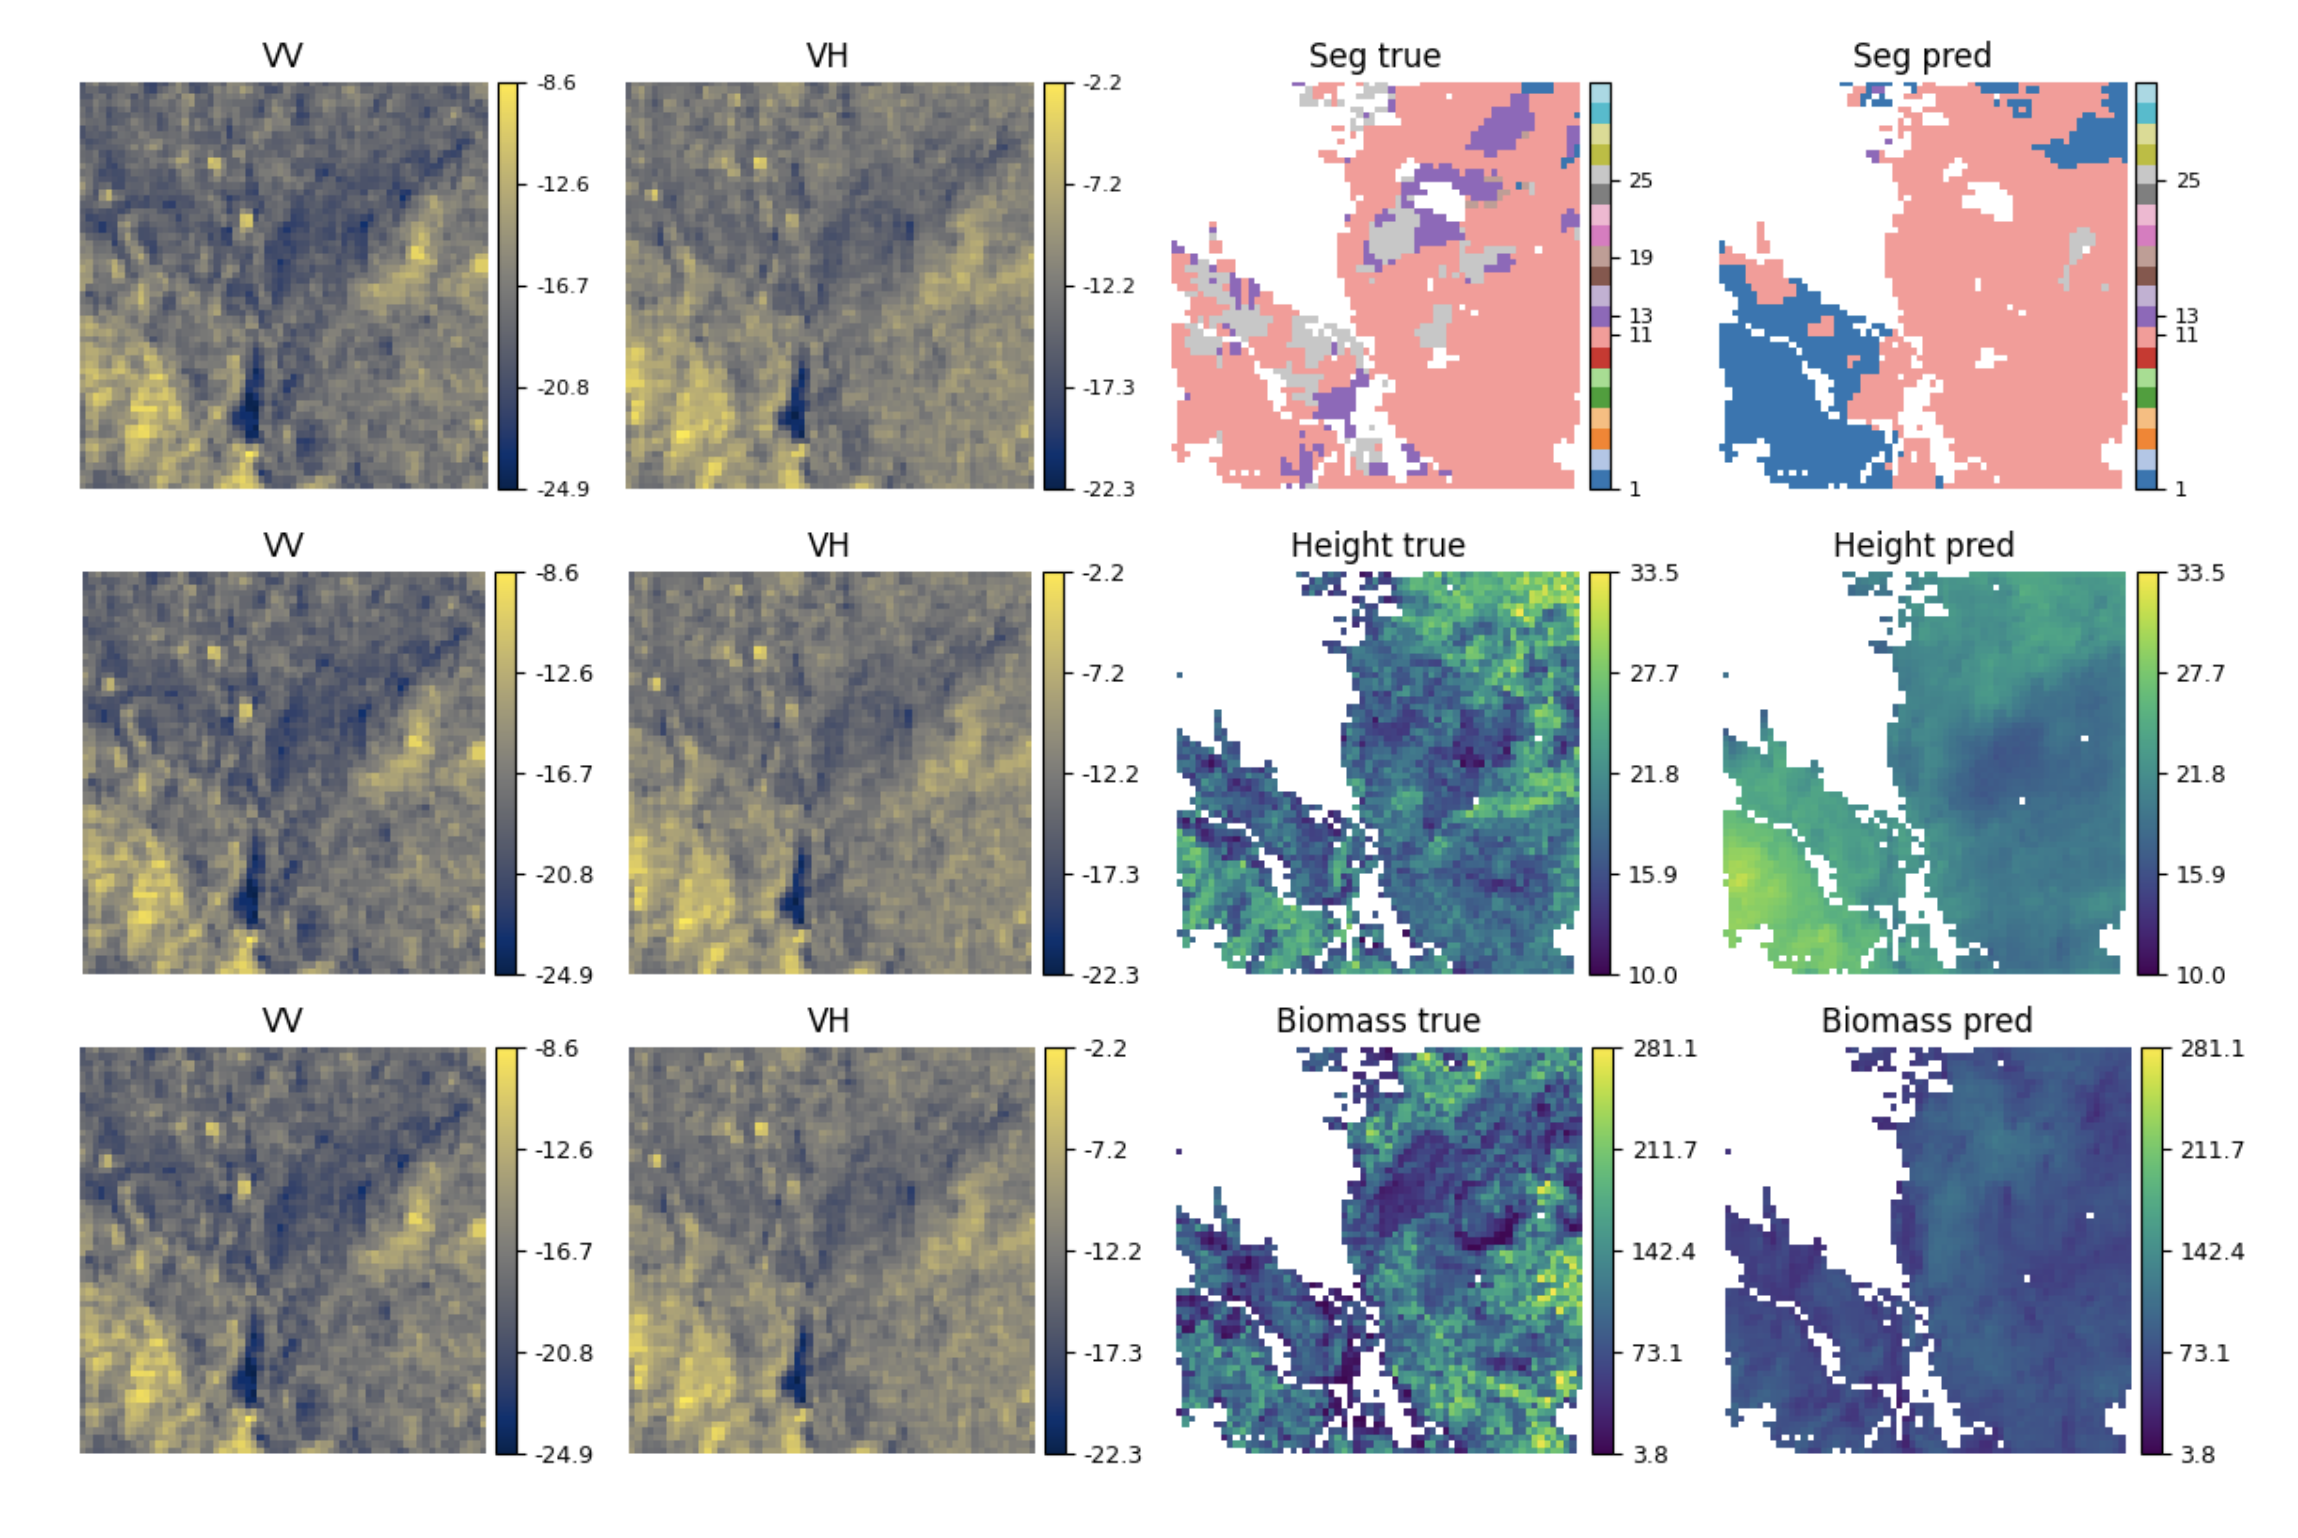
\includegraphics[width=0.9\textwidth]{mtl-all-tasks-samples.png}
    \caption[Multitask model predictions on iMAESTRO test set]{Multitask model predictions on iMAESTRO test set. Example predictions showing VV/VH input and predictions for all three tasks from the shared encoder architecture. The multitask model maintains comparable visual quality to single-task baselines while using a single shared encoder.}
    \label{fig:imaestro_mtl_samples}
\end{figure}

\begin{figure}[htbp]
    \centering
    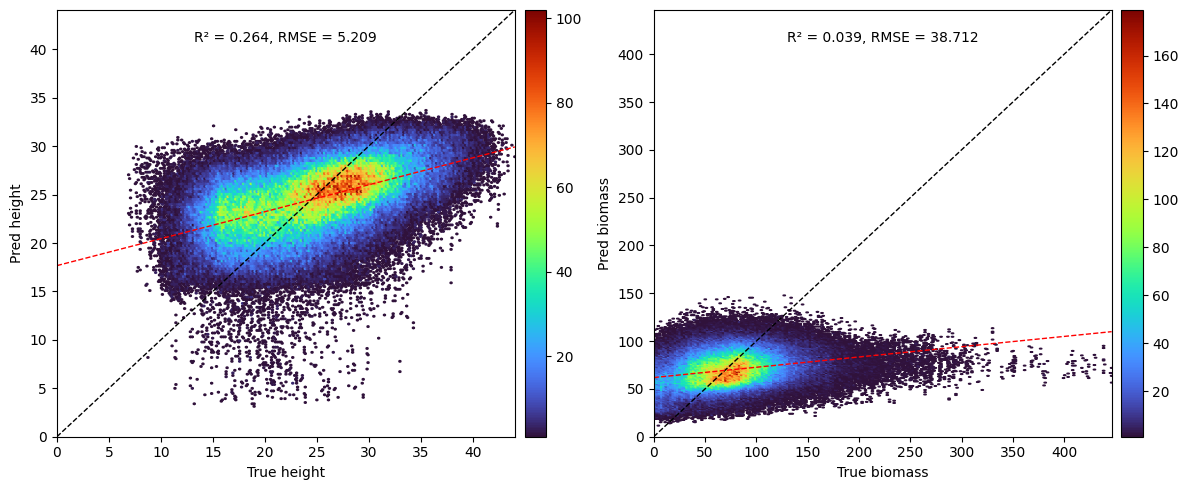
\includegraphics[width=0.9\textwidth]{height-biomass-scatter-plot.png}
    \caption[Height-biomass relationship in multitask predictions]{Height-biomass relationship in multitask predictions. Scatter plot showing the correlation between predicted height and biomass values, demonstrating that the allometric constraint successfully maintains the ecological relationship between these variables.}
    \label{fig:imaestro_height_biomass}
\end{figure}

Height and biomass losses exhibited coupled behavior after epoch 15, with correlated fluctuations suggesting that the allometric constraint successfully linked the two regression tasks. The validation metrics for all three tasks improved steadily until around epoch 35, and after segmentation and height metrics stabilized, biomass continued to increase slightly.

\subsection{Gradient and Representation Analysis}

\subsubsection{Gradient Alignment in the Shared Encoder}

\begin{figure}[htbp]
    \centering
    
\includegraphics[width=0.7\textwidth]{gradient-comparison.png}
    \caption[Gradient cosine similarity between task pairs in the shared encoder]{Gradient cosine similarity between task pairs in the shared encoder across training epochs. Positive values indicate aligned gradients where tasks agree on parameter updates; negative values indicate conflicting gradients where tasks push parameters in opposite directions.}
    \label{fig:imaestro_gradients}
\end{figure}

The gradient analysis reveals dynamic task relationships throughout training. In the first 15 epochs, all three task pairs exhibit highly variable gradient alignment with frequent sign changes, indicating tasks initially compete for shared encoder capacity. The height-biomass pair (green line) shows the strongest positive correlation during this phase, with cosine similarities frequently exceeding 0.6, suggesting these two regression tasks naturally share low-level feature requirements.

After epoch 15, gradient patterns stabilize. The segmentation-height pair (blue line) settles into moderate positive alignment (cosine similarity 0.4--0.7), indicating genus classification and height estimation benefit from similar mid-level features. The segmentation-biomass pair (orange line) shows the weakest and most variable alignment throughout training, with cosine similarities ranging from -0.3 to 0.6, suggesting genus classification and biomass estimation require partially conflicting features.

The height-biomass pair maintains strong positive alignment (0.4--0.9) after the initial training phase, particularly from epochs 20--40. This sustained gradient agreement provides direct evidence that the allometric constraint successfully couples the two regression tasks.

\subsubsection{Feature Similarity Across Decoder Layers}

\begin{figure}[htbp]
    \centering
    
\includegraphics[width=\textwidth]{cka.png}
    \caption[Centered Kernel Alignment (CKA) similarity between task-specific decoder representations]{Centered Kernel Alignment (CKA) similarity between task-specific decoder representations at different layers. Each heatmap shows CKA similarity between decoder layers of two tasks. Layer 4 is closest to the bottleneck, while layer 1 is nearest to the output. Higher CKA values (red) indicate more similar representations.}
    \label{fig:imaestro_cka}
\end{figure}

CKA analysis quantifies how similarly task-specific decoders transform shared encoder features. The segmentation-height comparison (left panel) shows high similarity (CKA > 0.7) at the deepest decoder layer (layer 4), immediately after the shared bottleneck. As we move toward shallower layers (layers 3, 2, 1), CKA similarity decreases progressively, reaching 0.51--0.66 at layer 3 and 0.51--0.54 at layers 2 and 1. This gradient of decreasing similarity demonstrates that decoders gradually specialize for their respective tasks.

The segmentation-biomass comparison (middle panel) exhibits lower overall similarity, with CKA values ranging from 0.25 to 0.51. The deepest layer (layer 4) shows moderate similarity (CKA $\approx$ 0.5), substantially lower than the segmentation-height pair, confirming biomass estimation requires fundamentally different feature processing than genus classification.

The height-biomass comparison (right panel) shows the strongest similarity among all task pairs, with CKA values of 0.77--0.81 at layer 4 and remaining high (0.64--0.81) through layers 3, 2, and 1. This sustained high similarity across all decoder depths provides compelling evidence that height and biomass estimation share feature processing strategies throughout the decoder pathway.

\begin{figure}[htbp]
    \centering
    
\includegraphics[width=\textwidth]{representations-across-layers.png}
    \caption[Layer-wise representation analysis across decoder depths]{Layer-wise representation analysis across decoder depths. Visualization of how task-specific representations evolve from the shared bottleneck through decoder layers, showing progressive specialization for each task while maintaining alignment for related tasks (height and biomass).}
    \label{fig:imaestro_representations}
\end{figure}

\subsection{Summary}

The iMAESTRO experiments tested multitask learning on larger patches ($64\times 64$ pixels) with three tasks: genus segmentation, canopy height regression, and biomass regression. The key experimental findings are:

First, baseline performance shows that all three tasks are learnable from SAR data, with segmentation achieving 63.8\% accuracy and height regression reaching $R^2 = 0.255$. Biomass regression shows weaker performance ($R^2 = 0.024$), reflecting both label quality issues and C-band SAR saturation at high biomass values (100-150 t/ha). The larger patch size compared to TreeSatAI-CHM provides more spatial context, leading to better absolute performance.

Second, the multitask model with allometric constraints improves both regression tasks while maintaining segmentation performance. Height $R^2$ increases from 0.255 to 0.265 (+3.7\%), and biomass $R^2$ increases from 0.024 to 0.039 (+62.5\% relative improvement). The allometric constraint (with weight $\lambda = 0.1$) couples height and biomass predictions, enforcing the ecological relationship $\log(B) = \alpha + \beta \times \log(H)$ with parameters $\alpha = 0.0673$ and $\beta = 2.5$.

Third, gradient analysis shows strong alignment between height and biomass tasks (cosine similarity 0.4-0.9 throughout training), confirming that the allometric constraint guides both tasks toward compatible feature learning. Segmentation shows weaker alignment with biomass, suggesting genus classification needs different features than continuous attribute estimation. The learned uncertainty parameters (1.0 for segmentation, 0.4 for height, 0.3 for biomass) reflect relative task difficulty and automatically balance task contributions.

Fourth, CKA analysis reveals how representations evolve through the network. The bottleneck shows high similarity across all task pairs (0.64-0.81), indicating shared abstract features. Similarity decreases through decoder layers as tasks specialize, but height-biomass similarity remains high (0.64-0.81 across all decoder layers) due to the allometric coupling. This sustained similarity provides evidence that physics-aware constraints maintain consistent representations throughout the network.

    \chapter{Discussion and Conclusion}
\label{chap:discussion}

This chapter connects the experimental findings back to the research questions from Chapter~\ref{chap:introduction}. The experiments tested multitask learning for forest monitoring using Sentinel-1 SAR data on two datasets: TreeSatAI-CHM (small patches, classification + height) and iMAESTRO (larger patches, segmentation + height + biomass with physics constraints).

\section{Answering the Research Questions}

\textbf{Question 1: Can TreeSatAI be extended with canopy height labels?}

Yes. The TreeSatAI benchmark was extended with height labels from German LiDAR data. The process generated canopy height models from terrain and surface elevation data, aligned them to the TreeSatAI grid, and combined them with Sentinel-1 backscatter. The resulting TreeSatAI-CHM dataset keeps the original species labels while adding pixel-level height information.

Validation confirmed the data quality. Negative values were removed, extremes were clipped, and height distributions matched expected ranges for German forests. Tests with Sentinel-2 optical data achieved much better performance (32.8\% classification, 5.78m RMSE for height), confirming the dataset contains real patterns and that modest SAR performance comes from radar's inherent limitations, not data problems.

\textbf{Question 2: How do shared encoders learn features for multiple tasks?}

The gradient and representation analyses show a clear pattern. Early encoder layers learn basic features like edges and textures that are mostly shared, though tasks sometimes conflict when they need different things. Middle layers learn forest structure features that align moderately well across tasks. The bottleneck learns abstract concepts that are strongly shared across related tasks.

Task-specific decoders then refine these shared features. CKA analysis in iMAESTRO shows similarity decreasing from bottleneck to output as tasks specialize. But height and biomass decoders stay highly similar throughout when coupled by the allometric constraint, showing that related tasks can maintain aligned features even during specialization.

\textbf{Question 3: When do gradient conflicts happen and how to manage them?}

Gradient analysis shows conflicts mainly occur in early encoder layers during initial training. This makes sense---classification wants edge-preserving features to distinguish genus boundaries, while regression wants smoothing features to reduce speckle noise.

As training continues, alignment improves, especially in deeper layers. The bottleneck shows the strongest agreement, meaning tasks agree on high-level concepts. Task-specific learning rates (TreeSatAI-CHM) and uncertainty weighting (iMAESTRO) successfully balance these competing needs. Height and biomass in iMAESTRO show particularly strong alignment, demonstrating that physics constraints can reduce conflicts by guiding tasks toward compatible goals.

\textbf{Question 4: Does multitask learning match or beat single-task baselines?}

Multitask learning achieves comparable or slightly better performance in both datasets:
\begin{itemize}
    \item TreeSatAI-CHM: Classification F1 improves from 12.61\% to 12.82\%, regression maintains similar performance ($R^2 = 0.033$ vs 0.042 baseline)
    \item iMAESTRO: Height $R^2$ improves from 0.255 to 0.265 (+3.7\%), biomass $R^2$ improves from 0.024 to 0.039 (+62.5\% relative)
\end{itemize}

The improvements are modest but consistent. This reflects C-band SAR's fundamental limits for these tasks, not multitask learning failures. TreeSatAI-CHM has tiny patches ($6\times 6$ pixels) limiting what can be learned, while iMAESTRO faces SAR saturation for high biomass.

Beyond raw numbers, multitask learning offers practical benefits. One shared encoder serves multiple tasks, cutting parameters and inference time versus separate models. The shared encoder acts as regularization, preventing overfitting to any single task. Physics constraints ensure predictions follow known ecological relationships, improving reliability even when accuracy is limited.

\textbf{Question 5: Can physics-aware constraints improve multitask learning?}

Yes. The allometric constraint in iMAESTRO successfully couples height and biomass prediction. High gradient alignment (cosine similarity 0.4-0.9) and CKA similarity (0.64-0.81 across decoder layers) show the constraint guides both tasks toward consistent predictions. While absolute performance gains are modest, the constraint helps the model learn structured predictions that respect the ecological relationship between height and biomass.

\section{Key Takeaways}

The two datasets provided different but complementary insights into how multitask learning works for forest monitoring from SAR data.

\textbf{Main challenges and solutions.} The biggest challenge across both datasets was balancing tasks with different loss scales. Classification uses binary cross-entropy (values around 0.3-0.8) while regression uses RMSE (values around 5-15m), creating a two-order-of-magnitude difference that makes optimization difficult. When tasks operate on such different scales, the optimizer struggles to find learning rates that work well for both---a rate suitable for one task often causes the other to diverge or stagnate.

Two approaches successfully addressed this challenge. In TreeSatAI-CHM, task-specific learning rates were applied to different parameter groups (shared encoder, classification head, regression decoder). The encoder used $5\times 10^{-6}$, classification head $5\times 10^{-6}$, and regression decoder $5\times 10^{-5}$. This allowed each component to learn at an appropriate pace. In iMAESTRO, uncertainty weighting automatically balanced task contributions by learning uncertainty parameters ($\sigma$) for each task. The model learned to down-weight tasks with higher uncertainty, effectively normalizing their loss contributions. Both approaches require careful tuning (task-specific rates) or additional learnable parameters (uncertainty weights), but proved effective in practice.

Task asymmetry was another consistent pattern. Regression tasks benefited more from shared encoders than classification tasks. This asymmetry has multiple causes. First, regression's continuous outputs provide stronger training signals than classification's discrete predictions. Second, output granularity matters---in TreeSatAI-CHM, classification makes one prediction per $6\times 6$ patch while regression makes 36 (one per pixel), so regression contributes much more gradient per sample. Third, regression tasks may have more compatible feature requirements across different prediction targets (height and biomass both relate to forest structure), while classification requires genus-specific discriminative features that don't transfer as well.

Both datasets also face inherent data limits that constrain absolute performance. TreeSatAI-CHM has tiny patches ($6\times 6$ pixels) with little spatial context---at 10m resolution, this covers only 60m $\times$ 60m on the ground, barely enough to capture a few tree crowns. The small patch size limits what spatial patterns can be learned. iMAESTRO has larger patches but faces label quality issues (synthetic data from forest simulators) and C-band SAR saturation for high biomass (around 100-150 t/ha). SAR backscatter saturates because the signal penetration depth becomes limited in dense forests, making it impossible to distinguish biomass variations above the saturation threshold. These fundamental limits cap performance regardless of the learning approach. C-band SAR simply has inherent physical limits for species classification (lacks spectral information) and high biomass estimation (saturation effects).

\textbf{Effective approaches.} Despite these challenges, several strategies proved reliable across both datasets. Gradient analysis revealed that tasks generally align in deeper layers while occasionally conflicting in early layers. This pattern held for both datasets and informed architectural choices. The shared encoder provided regularization benefits without causing major negative transfer---multitask models matched or slightly exceeded single-task baselines in both experiments.

The ablation study in TreeSatAI-CHM showed that simpler architectures work better with limited data. Cross-stitch networks and cross-attention both performed worse than plain hard sharing, likely because the small dataset and tiny patches can't leverage the extra parameters effectively. This suggests model complexity should match data availability.

Physics-aware constraints proved valuable in iMAESTRO. The allometric constraint coupled height and biomass prediction, leading to strong gradient alignment (0.4-0.9) and representation similarity (0.64-0.81) between these tasks. While absolute performance gains were modest, the constraint helped the model learn predictions that respect ecological relationships.

\textbf{Key contributions.} This work makes several contributions to multitask learning for forest monitoring:

First, the TreeSatAI benchmark was extended with canopy height labels from German LiDAR data, creating TreeSatAI-CHM for multitask learning research. The dataset keeps the original spatial coverage and species labels while adding pixel-level height information.

Second, multitask architectures were developed and tested for combining classification and regression from SAR data. The MultiTaskUNet with shared encoder and task-specific decoders provides a baseline for future work.

Third, task interactions were systematically analyzed using gradient cosine similarity and centered kernel alignment (CKA). These analyses show where tasks align (deeper layers) and conflict (early layers), giving quantitative evidence of how multitask learning works.

Fourth, three parameter sharing strategies (hard sharing, cross-stitch, cross-attention) were compared, showing that simpler architectures work better with limited data. This informs architectural choices for similar problems.

Fifth, physics-aware multitask learning was demonstrated by incorporating allometric constraints. The sustained high alignment between height and biomass tasks shows that domain knowledge can guide feature learning toward consistent, plausible predictions.

Finally, the experiments showed that multitask learning is practically feasible for forest monitoring from SAR data. Despite challenges like loss scale mismatch and occasional gradient conflicts, multitask models match baseline performance while using fewer parameters and less inference time. This makes multitask learning viable for operational applications where deploying multiple single-task models would be expensive.

\section{Looking Forward}

Several directions could build on this work:

\textbf{Architecture Design.} The gradient analysis suggests that letting tasks specialize in early layers while sharing deeper layers could reduce conflicts. Architectures like cross-stitch networks or progressive layer sharing might work well with larger datasets. The ablation study showed these approaches underperform with limited data, but they could prove valuable at scale.

\textbf{Physics Constraints.} The allometric constraint successfully couples height and biomass, but additional physical relationships could be incorporated. For example, genus-specific allometric equations would provide stronger supervision than the generic equation used here. Other relationships like crown diameter to height or age to biomass could also be explored.

\textbf{Data.} Both experiments were limited by training data size. Larger datasets with more diverse forest types and conditions would enable more robust learning and better generalization. The computational efficiency of multitask learning becomes more valuable at scale, where deploying multiple single-task models gets expensive.

\textbf{Final thoughts.} This thesis investigated multitask learning for forest monitoring from Sentinel-1 SAR data. The main finding is that multitask learning works for this problem. While performance improvements over single-task baselines are modest, multitask learning offers computational efficiency, regularization benefits, and the ability to incorporate domain knowledge through physics constraints.

The gradient and representation analyses show how shared architectures learn hierarchical features. Low-level features are mostly shared across tasks, while high-level features progressively specialize. Physics constraints can maintain alignment between related tasks even during specialization.

The challenges identified here, such as loss scale mismatch, task asymmetry, and datalimitations, they have solutions. Task-specific learning rates, uncertainty weighting, and physics constraints all work to address these issues. The modest performance improvements reflect fundamental sensor and data limits, not multitask learning failures. C-band SAR simply has inherent limits for species classification and high biomass estimation.

For operational forest monitoring, multitask learning offers a practical solution. One model can estimate multiple forest attributes, cutting computational costs while maintaining prediction quality. Physics constraints ensure predictions follow ecological relationships, improving reliability for decision-making. As datasets grow and sensors improve, multitask learning provides a framework to leverage these advances efficiently.

    \appendix

    % \input{./chapters/Anhang}

% ---------------------------------------------------------------
\bibliographystyle{plainnat}
%\bibliographystyle{abbrv}
%\bibliographystyle{alpha}
\renewcommand\bibname{References}
\bibliography{bib/export-data}

\backmatter

\end{document}
